%! Author = Nikolay Stanishev
%! Date = 21.05.22

% Preamble
\documentclass{article}

% Language setting
\usepackage[utf8]{inputenc}
\usepackage[bulgarian]{babel}

% Page numbering
\usepackage{etoolbox,titling}
\makeatletter
\patchcmd{\titlepage}{\setcounter{page}\@ne}{}{\message {Successfully patched titlepage.}}{\message {Failed to patch titlepage.}}
\makeatother

% Math stuff
\usepackage{amsmath, amssymb, bm}
\usepackage{amsfonts}

% Set page size and margins
\usepackage[colorlinks=true, allcolors=blue]{hyperref}\usepackage{geometry}
\geometry{verbose,tmargin=3cm,bmargin=3cm,lmargin=3cm,rmargin=3cm}

% Setup figures
\usepackage{caption}
\usepackage{subcaption}
\usepackage{graphicx}
\usepackage{float,graphicx}
\graphicspath{ {./images/} }

% Add indentation for all paragraphs
\usepackage[skip=10pt plus1pt, indent=20pt]{parskip}
\usepackage{indentfirst}

% Set font size to 13pt
\usepackage[fontsize=13pt]{scrextend}

\usepackage{etoolbox}
\patchcmd{\thebibliography}{\section*}{\section}{}{}
\usepackage[superscript,biblabel]{cite}

% Create sections list
\usepackage{titlesec}
\usepackage{hyperref}

\titleclass{\subsubsubsection}{straight}[\subsection]

\newcounter{subsubsubsection}[subsubsection]
\renewcommand\thesubsubsubsection{\thesubsubsection.\arabic{subsubsubsection}}
\renewcommand\theparagraph{\thesubsubsubsection.\arabic{paragraph}} % optional; useful if paragraphs are to be numbered

\titleformat{\subsubsubsection}
{\normalfont\normalsize\bfseries}{\thesubsubsubsection}{1em}{}
\titlespacing*{\subsubsubsection}
{0pt}{3.25ex plus 1ex minus .2ex}{1.5ex plus .2ex}

\makeatletter
\renewcommand\paragraph{\@startsection{paragraph}{5}{\z@}%
{3.25ex \@plus1ex \@minus.2ex}%
{-1em}%
{\normalfont\normalsize\bfseries}}
\renewcommand\subparagraph{\@startsection{subparagraph}{6}{\parindent}%
{3.25ex \@plus1ex \@minus .2ex}%
{-1em}%
{\normalfont\normalsize\bfseries}}
\def\toclevel@subsubsubsection{4}
\def\toclevel@paragraph{5}
\def\toclevel@paragraph{6}
\def\l@subsubsubsection{\@dottedtocline{4}{7em}{4em}}
\def\l@paragraph{\@dottedtocline{5}{10em}{5em}}
\def\l@subparagraph{\@dottedtocline{6}{14em}{6em}}
\makeatother

\setcounter{secnumdepth}{5}
\setcounter{tocdepth}{5}

% Create quotation
\makeatletter
\newenvironment{chapquote}[2][2em]
{\setlength{\@tempdima}{#1}%
\def\chapquote@author{#2}%
\parshape 1 \@tempdima \dimexpr\textwidth-2\@tempdima\relax%
\itshape}
{\par\normalfont\hfill--\ \chapquote@author\hspace*{\@tempdima}\par\bigskip}
\makeatother

% Algorithms
\usepackage{algpseudocode}
\usepackage{algorithm}
\usepackage{algorithm,algorithmicx,setspace}
\newcommand{\stepsize}{\alpha}
\newcommand{\params}{\mathbf{\theta}}
\newcommand{\entropy}{S}
\newcommand{\vI}{\mathbf{I}}
\newcommand{\gradparams}{\nabla L(\params_t, t)}
\newcommand{\N}[2]{\mathcal{N}\!\left(#1,#2\right)}
\newcommand{\vg}{\mathbf{g}}
\newcommand{\vr}{\mathbf{r}}
\newcommand{\tra}{^{\mathsf{T}}}
\DeclareMathOperator*{\argmin}{arg\,min}
\newcommand{\R}{\ensuremath{\mathbb{R}}}
\newcommand{\ti}{_{t+1}}

% Include pdf
\usepackage{pdfpages}

% Paragraph add new line and ident
\makeatletter
\renewcommand\listoffigures{%
    \section{\listfigurename}%
    \@mkboth{\MakeUppercase\listfigurename}%
    {\MakeUppercase\listfigurename}%
    \@starttoc{lof}%
}
\makeatother

\makeatletter
\renewcommand\listoftables{%
    \section{\listtablename}%
    \@mkboth{\MakeUppercase\listtablename}%
    {\MakeUppercase\listtablename}%
    \@starttoc{lot}%
}
\makeatother

\makeatletter
\renewcommand{\paragraph}{\@startsection{paragraph}{4}{0ex}%
{-3.25ex plus -1ex minus -0.2ex}%
{1.5ex plus 0.2ex}%
{\normalfont\normalsize\bfseries}}
\makeatother

% code blocks
\usepackage{listings}
\usepackage{xcolor}

\definecolor{codegreen}{rgb}{0,0.6,0}
\definecolor{codegray}{rgb}{0.5,0.5,0.5}
\definecolor{codepurple}{rgb}{0.58,0,0.82}
\definecolor{backcolour}{rgb}{0.95,0.95,0.92}

\lstdefinestyle{mystyle}{
    backgroundcolor=\color{backcolour},
    commentstyle=\color{codegreen},
    keywordstyle=\color{magenta},
    numberstyle=\tiny\color{codegray},
    stringstyle=\color{codepurple},
    basicstyle=\ttfamily\footnotesize,
    breakatwhitespace=false,
    breaklines=true,
    captionpos=b,
    keepspaces=true,
    numbers=left,
    numbersep=5pt,
    showspaces=false,
    showstringspaces=false,
    showtabs=false,
    tabsize=2
}

\lstset{style=mystyle}

\usepackage{color}
\definecolor{lightgray}{rgb}{.9,.9,.9}
\definecolor{darkgray}{rgb}{.4,.4,.4}
\definecolor{purple}{rgb}{0.65, 0.12, 0.82}

\lstdefinelanguage{JavaScript}{
    keywords={typeof, new, true, false, catch, function, return, null, catch, switch, var, if, in, while, do, else, case, break},
    keywordstyle=\color{blue}\bfseries,
    ndkeywords={class, export, boolean, throw, implements, import, this},
    ndkeywordstyle=\color{darkgray}\bfseries,
    identifierstyle=\color{black},
    sensitive=false,
    comment=[l]{//},
    morecomment=[s]{/*}{*/},
    commentstyle=\color{purple}\ttfamily,
    stringstyle=\color{red}\ttfamily,
    morestring=[b]',
    morestring=[b]"
}

% Make sections
\renewcommand{\listalgorithmname}{\thesection\hspace{5mm}Списък на алгоритмите}
\renewcommand\lstlistingname{Код}
\renewcommand\lstlistlistingname{\thesection\hspace{5mm}Списък на блоковете с код}

% REST API
\usepackage{rest-api}

% tables
\usepackage{multirow}
\usepackage{adjustbox}

% charts
\usepackage{pgfplots}

% Document
\begin{document}

    \begin{titlepage}
        \vspace*{-3cm}\hspace*{15cm}\includegraphics[width=64px, keepaspectratio]{title-page/tu-logo.png}
        \begin{center}
            \textsc{{\textbf{ТЕХНИЧЕСКИ УНИВЕРСИТЕТ - СОФИЯ} \\}}
            \textsc{{\textbf{ФАКУЛТЕТ КОМПЮТЪРНИ СИСТЕМИ И ТЕХНОЛОГИИ} \\}}
            \vspace{40mm}
            \huge{\textbf{ДИПЛОМНА РАБОТА} \\}
            \vspace{15mm}
            \textnormal{ \LARGE{Проектиране и разработване на система за анализ на публично мнение на базата на данни от социални платформи\\}}
        \end{center}
        \vspace{20mm}
        \begin{minipage}[t]{0.47\textwidth}
            \textnormal{\large{\bf Дипломант:\\}}
            {\large Николай Станишев}
        \end{minipage}\hfill\begin{minipage}[t]{0.47\textwidth}
                                \raggedleft
                                \textnormal{\large{\bf Научен ръководител:\\}}
                                {\large проф. д-р Милена Лазарова}
        \end{minipage}
        \vspace{50mm}

        \begin{center}
        {\large{СОФИЯ, България}}
            \\
            {\large{2022 г.}}
        \end{center}
    \end{titlepage}

    \addcontentsline{toc}{section}{Дипломно задание}
    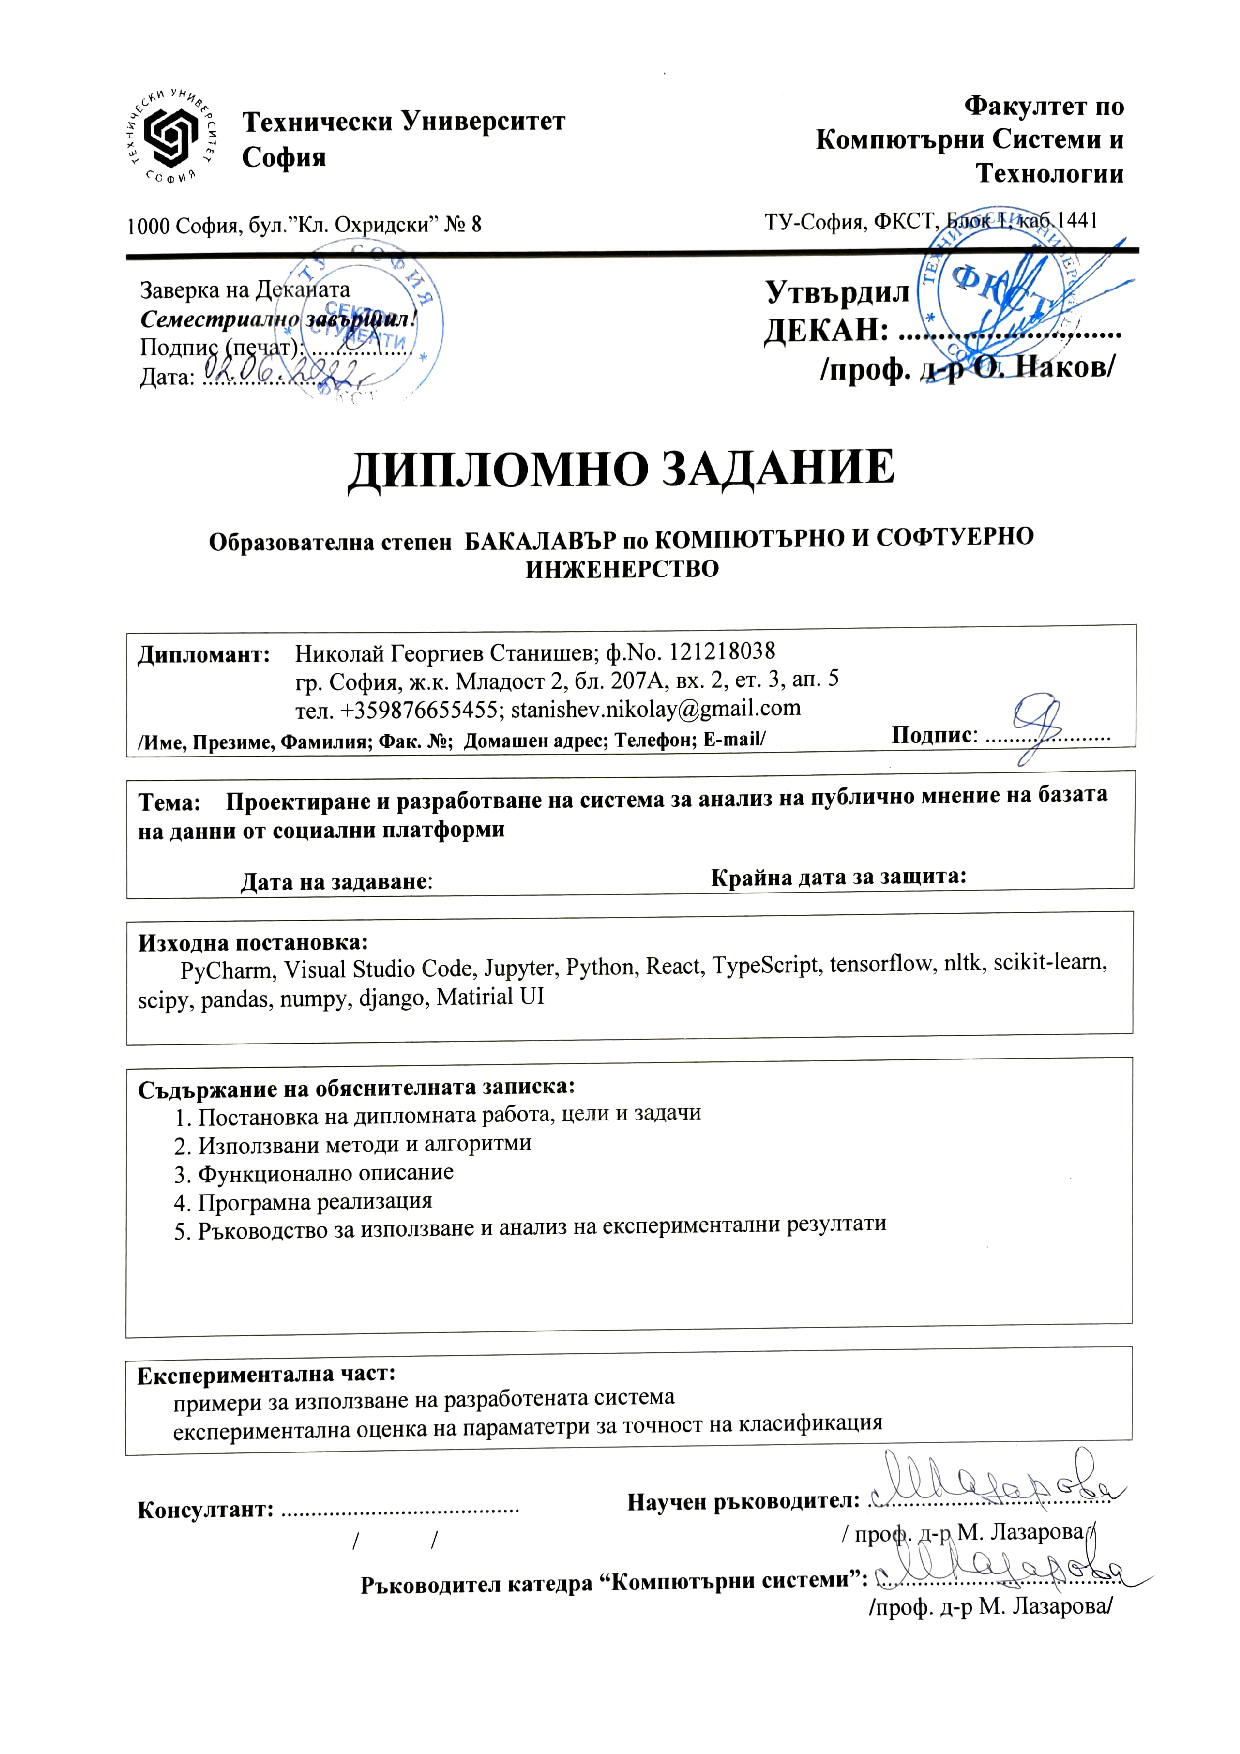
\includepdf[pages=-]{diploma-assigment.pdf}

    \addcontentsline{toc}{section}{Декларация за авторство}
    \includepdf[pages=-]{author-declaration.pdf}

    \newpage\tableofcontents

    \newpage


    \section{Увод}

    В последните години данните са придобили особено значение в сферата на информационните технологии. Много от
    разработваните програмни системи са фокусирани върху тях, както и голяма част от бизнесът в тази сфера изкарва своите
    доходи чрез тях. Това развитие се дължи до голяма степен на изследванията свързани с обработката на сурови данни,
    които не носят никаква информация до структурирани резултати, които може да бъдат интерпретирани.

    Този интерес към данните се дължи на две основни групи от причини. Първата е увеличението на базата от потребители на
    повечето от приложенията, а другата е развитието на хардуерните ресурси. Ръста на потребителите влияе благосклонно на
    генерирането на повече данни, от количествена гледна точка. Развитието на хардуерните ресурси позволява по-бързото
    изготвяне на експерименти. Повечето от използваните концепции за анализ на данни са измислени през миналият век, но
    развитието на хардуерните ресурси и наличието на повече данни, позволява навлизането на повече хора в този под дял на
    компютърните науки.

    Публичното мнение е нещо, което може да бъде използвано за много причини. Примери за такива са валидиране на резултати
    от маркетингови кампании, нагласата на обществото към нов продукт на пазара или към събития свързани с известни
    личности. Друг пример, където публичното мнение води хода на събитията е политиката.

    За изготвяне на анализи на база публично мнение има различни утвърдени канали. Един от често използваните подходи е
    набирането им, чрез анкети. Този подход има много недостатъци. Друг канал може да бъдат социалните мрежи. Този начин за
    набиране на данни има много потенциал. Това се дължи на големият дял хора, които използват една или друга социална
    платформа. На база проучване от Април 2022 г. е установено, че повече от 58\% от всички хора в глобален план използват
    някоя от популярните социални платформи. \cite{social-media-users}

    Целта на тази дипломна работа е да разгледа тенденциите споменати по-горе. За осъществяването на тази цел ще се
    разработи система, чрез която лесно ще може да се анализират обществените нагласи, чрез задаване на критерии за търсене
    в социални мрежи, за които е изготвен интерфейс за комуникация. Следващата стъпка отредена на тази система е да
    анализира всеки отделен пост за неговият клас - дали е позитивен или негативен, както и изготвянето на кратко обобщение
    на база всички постове. Тези статистики ще бъдат предоставени на потребителя, който ще може да прави изводи на тяхна
    база.

    \newpage


    \section{Постановка на дипломната работа, цели и задачи}

    \subsection{Постановка}

    \subsubsection{Сантиментно класифициране на текст}

    Сантиментният класифициращ метод е директно насочен към класификацията на документи, при които се приема че може да се
    свържат надежди етикети. В простият случай сантиментното класифициране е дву или три класов проблем, където сантиментите
    са ПОЗИТИВЕН, НЕГАТИВЕН и възможно НЕИЗВЕСТЕН. Тези анотации може да бъдат зададени на ръка или чрез някоя от чертите на
    документите. \cite{intro-to-nlp-mit}

    \subsubsection{Обобщаване на текст}

    Обобщаването на текст е проблем свързан с конвертирането на дълъг текст в по-кратък, докато се запазва неговият смисъл
    - основни факти, събития, идеи и сантимент от оригиналният. Има два вида обобщаване - с извличане и абстрактно. При
    това с извличане резултатът е под сборище на оригиналният текст. Докато при абстрактното резултатът е създаден от
    нулата, чрез перифразиране на началната поредица. \cite{intro-to-nlp-mit}

    \subsubsection{Анализ на съществуващи решения}

    \subsubsubsection{Анализиране на публично мнение на база социални платформи}

    Към днешна дата анализирането на публично мнение на база социални платформи се извършва тясно фокусирано върху проблемът
    на интерес. Основният интерес, който има към подобни проучвания е за президентските избори в Съединените Американски
    Щати.

    \paragraph{Проучване за президенските избори в САЩ през 2016 г.}

    Мониторинга на трендовете в публичното мнение на база социални платформи има потенциала да замени досегашният начин,
    чрез анкети.

    Данните за това проучване са взети от Twitter в периода от 1-ви септември до 8-ми ноември 2016 г. Размерът им е в
    рамките на 2.2 милиона поста. За анализът е използван opinion-oriented word embedding (OOWE). \cite{us-election-2016}

    \begin{figure}[H]
        \centering
        \captionsetup{justification=centering}
        \includegraphics{chapter-02/us-election-2016.png}
        \caption{Процес на анализиране на президентските избори в САЩ през 2016 г.}
    \end{figure}

    \begin{figure}[H]
        \centering
        \captionsetup{justification=centering}
        \includegraphics[width=400px, keepaspectratio]{chapter-02/us-election-2016-results.png}
        \caption{Резултати от анализирането на президентските избори в САЩ през 2016 г. Червените точки са гласове за Тръмп,
            а червените за Клинтън в зададените щати.}
    \end{figure}

    \subsubsubsection{Модели за обработка и анализиране на текст}

    \paragraph{T5}

    T5 е модел за обработка на текст. Този модел следва архитектурата на енкодер-декодер трансформър. Съкращението T5 идва
    от Text-to-Text Transfer Transformer. Задачите, които може да изпълнява са машинен превод, отговаряне на въпроси,
    обобщаване на текст, класификация на текст, както и други задачи свързани с анализирането на текст. Тези задачи могат
    да бъдат обобщени като обработване на някакъв текстови вход от T5 моделът до генерирането на желан текст на изходът му.

    Тренирането на този модел е осъществено на 1024 TPU v3 чипове. Броят на тренирани параметри на този модел варира от 220
    милиона до 11 милиарда в зависимост от версията му. \cite{t5}

    \begin{figure}[H]
        \centering
        \captionsetup{justification=centering}
        \includegraphics[width=450px, keepaspectratio]{chapter-02/t5.png}
        \caption{Архитектура на моделът T5}
    \end{figure}

    \paragraph{BERT}

    BERT представлява репрезентационнен езиков модел. Зад абревиатурата BERT седи Bidirectional Encoder Representations
    from Transformers. От името му може да се разбере, че архитектурата му е много слоен двупосочен трансформърен енкодер.
    Броят на параметрите му варира от 110 до 340 милиона. \cite{bert}

    \begin{figure}[H]
        \centering
        \captionsetup{justification=centering}
        \includegraphics[width=450px, keepaspectratio]{chapter-02/bert.png}
        \caption{Архитектура на моделът BERT}
    \end{figure}

    \paragraph{GPT-3}

    GPT-3 е третата версия на GPT езиковият модел. Архитектурата на този модел стъпва върху трансформърите и ги надгражда.
    Той съдържа 175 милиарда параметъра, което е 10 пъти повече от всеки езиков модел преди него. Този модел е трениран на
    Common Crawl наборът от данни. \cite{gpt-3}

    \begin{figure}[H]
        \centering
        \captionsetup{justification=centering}
        \includegraphics[width=250px, keepaspectratio]{chapter-02/gpt-3.png}
        \caption{Архитектура на моделът GPT-3}
    \end{figure}

    \subsection{Цели и задачи}

    Целта на дипломната работа е да анализира и създаде система, чрез която ще може да се анализира публично мнение от
    различни източници. Източниците, които са фокус на тази работа са социални платформи. За демонстрация на работата на
    тази дипломна работа ще бъде използвана платформата Twitter.

    Анализът на публичното мнение ще се изготвя на база зададени елементи от платформите. В случаят на Twiiter това ще
    бъдат постове на потретилите ѝ - туитове. Изборът на тези елементи ще бъде оставен на потребителите на платформата,
    които ще имат възможност да ги филтрират по зададени от тях филтри. Този анализ ще върне като резултат репорт, който ще
    включва сантиментен анализ на отделните елементи, както и обобщаване на всички получени данни.

    Задачите, които ще бъдат изпълнени в тази работа са:

    \begin{itemize}
        \item Изготвяне на модел със свойство да изготвя сантиментен анализ.
        \item Използване на готов модел за обобщаване на много текстови елементи.
        \item Изготвяне на потребителски интерфейс представляващ интернет приложение, който ще може да извлича и оценя
        данни от социалната платформа Twitter.
    \end{itemize}

    \newpage


    \section{Използвани методи и алгоритми}

    \subsection{Машинно самообучение}

    Машинното самообучение е способността на компютрите да могат да се учат от данни.

    Ето една по-обща дефиниция:

    \begin{chapquote}{Arthur Samuel, \textit{1959}}
        ``Machine learning is the field of study that gives computers the ability to learn without being
        explicitly programmed.''
    \end{chapquote}

    И още една по инженерно ориентирана:

    \begin{chapquote}{Tom Mitchell, \textit{1997} \cite{hands-on-ml}}
        ``A computer program is said to learn from experience E with respect to some task T and some performance measure P,
        if its performance on T, as measured by P, improves with experience E.''
    \end{chapquote}

    Машинното самообучение се използва за извличане на знание от данни. То е пресечна точка на статистиката, изкуствения
    интелект и компютърната наука. Приложението му през последните години е навлязло много силно в ежедневието ни.
    \cite{intro-to-ml}

    \subsection{Контролирано машшино самообучение}

    Данните за трениране предоставени на алгоритъма за Контролираното Машинно самообучение включват в себе си и отговорите,
    наречени етикети. \cite{hands-on-ml} То се използва, когато искаме на направим предположение на база на някакви данни.
    Основните проблеми, с които се сблъсква Контролираното Машинно самообучение са регресия и класификация. За регресията
    целта ни е да правим непрекъснати предположения, а при класификацията целта ни е да направим предположение за някакъв
    клас, който присъства в някакъв списък от предварително зададени класове. \cite{intro-to-ml}

    \subsection{Дълбоко самообучение}

    Дълбокото самообучение е част от Машинното самообучение, която използва Изкуствени невронни мрежи частично вдъхновени
    от структурата на невроните намиращи се в човешкия мозък. \cite{deep-learning-keras} Изкуствените невронни мрежи са в
    сърцевината на Дълбокото самообучение. Те са гъвкави, мощни и мащабируеми, което ги прави идеални за големи и
    изключително сложни проблеми свързани с Машинното самообучение. \cite{hands-on-ml}

    \begin{figure}[H]
        \centering
        \captionsetup{justification=centering}
        \includegraphics{chapter-03/deep-learning.png}
        \caption{Връзката между Дълбокото самообучение, Машинното самообучение и Изкуствения интелект}
    \end{figure}

    Дълбокото самообучение е приложимо в много области свързани със снимки, текст, видео, говора и зрението. Освен многото
    области, в които е приложимо успехът му идва и от големите количества данни, които са достъпни и от увеличението на
    изчислителната мощност.

    Изкуствените невронни мрежи са вдъхновени от изучаването на централната нервна система на бозайниците. Всяка мрежа е
    съставена от взаимно свързани неврони, организирани в слоеве, които обменят информация. \cite{deep-learning-keras}

    \subsection{Natural Language Processing - NLP}

    NLP е множество от методи, които правят възможни човешките езици да бъдат разбирани от компютрите. През изминалото
    десетилетие, обработката на натурални езици е внедрена в ежедневието ни. Някой от задачите на NLP варират от
    автоматичен машинен превод, през класификацията на текстове и търсещи алгоритми до системи, с които може да
    комуникираме.

    Тези разнообразни приложения са базирани на множество от идеи, лежащи на алгоритми, лингвистика, логика, статистика и
    други елементи. \cite{intro-to-nlp-mit}

    \subsubsection{Първоначално почиствне на данните}

    \subsubsubsection{Стемиране}

    Стемирането е процес, при който се премахват приставките и наставките на думи. За целта се прилагат серия от замени с
    регулярни изрази. \cite{intro-to-nlp-mit}

    \subsubsubsection{Лематизиране}

    Лематизирането е процес, при който се идентифицира коренът на думите. Целта на този процес е да премахне грешката от
    обобщаването направено от стемирането. \cite{intro-to-nlp-mit}

    \subsubsection{Токенизиране}

    Токенизирането е един от по-лесните проблеми за разрешаване в обработката на натурални езици. Неговата цел е да
    преобразува текста в поредица от отделни токени. \cite{intro-to-nlp-mit}

    \subsubsection{Word2Vec}

    Word2Vec е алгоритъм, който има за цел да репрезентира думите, като ембединги. Ембедингите представляват къси и плътни
    вектори. Измеренията на ембединг вектора - $d$ обикновенно варират от 50 до 1000, за разлика от другите методи, при
    които се репрезентира цялата граматика - $V$, където измеренията са $|V|$. Ембедингите нямат ясна интерпретация. За
    разлика от другите методи за репрезентация на думи тук в стойностите на резултата няма да има много нули.

    Един от проблемите, които разрешават ембедингите е прекомерното надграждане. Друга сила, която притежават е хващането
    на синонимност.

    Начинът по който работи Word2Vec не като брои думи намиращи се около думата ни на интерес, а е чрез трениране на
    класификатор, който има следната задача - Думата $w$, колко вероятно е да се появи около думата на интерес. Тук не
    интересува резултатите от този модел, а ни интересуват неговите тежести, които са ембедингите на думите.
    \cite{intro-to-nlp-mit}

    \subsection{Архитектури на Невронни Мрежа}

    \subsubsection{Feed-Forward Невронна Мрежа}

    Feed-Forward невронната мрежа е тази с възможно най-проста архитектура. Тя представлява многослойна мрежа, при която
    елементите не са свързани с цикли по между си. Изходът на един елемент от едно ниво е вход на всички елементи от
    по-горно ниво. Елементите на такава мрежа, може да бъдат вход, скрит елемент или изход. \cite{intro-to-nlp-stanford}

    \begin{figure}[H]
        \centering
        \captionsetup{justification=centering}
        \includegraphics[width=450px, keepaspectratio]{chapter-03/feed-forward.png}
        \caption{Примерна архитектура на Feed-Forward невронна мрежа}
    \end{figure}

    \subsubsection{Recurrent Neural Network - RNN}

    RNN представлява невронна мрежа, която има цикли между нейните връзки. Това е невронна мрежа, при която стойността на
    входа на някой от елементите ѝ е директно или не директно зависима от стойността на друг предишен елемент.
    \cite{intro-to-nlp-stanford}

    \begin{figure}[H]
        \centering
        \captionsetup{justification=centering}
        \includegraphics[width=450px, keepaspectratio]{chapter-03/rnn.png}
        \caption{RNN клетка}
    \end{figure}

    \subsubsection{Long short-term memory - LSTM}

    LSTM е въведен през 1997 от Хочреитер и Шмидхъбер. Той е вариант на RNN, който има повече предимства в някой области на
    приложение. Моделът увеличава скритото състояние $h_m$ с паметна клетка $c_m$. Стойността на тази паметна клетка на
    всяко време $m$ се изчислява от сумата на предната и стойност $c_{m{-}1}$ и на опресняването $\tilde{c}_m$, което на
    своя ръка се изчислява от текущият вход $x_m$ и предното скрито състояние $h_{m{-}1}$. Следващото скрито състояние
    $h_m$ се изчислява от паметната клетка. Поради не предаването на паметната клетка през не линейни мачкащи функции по
    време на опресняването е възможно запазването и предаването на информация напред в невронната мрежа.
    \cite{intro-to-nlp-mit}

    \begin{figure}[H]
        \centering
        \captionsetup{justification=centering}
        \includegraphics[width=450px, keepaspectratio]{chapter-03/lstm.png}
        \caption{LSTM клетка}
    \end{figure}

    \subsubsection{BiLSTM}

    BiLSTM архитектурата надгражда LSTM. Тя се фокусира върху един от съществените проблеми на LSTM и го разрешава. Този
    проблем възниква от това, че моделите на LSTM вървят от ляво на дясно. В BiLSTM решението за думата $w_i$, използва,
    както и тагове от предните думи, така и такива от бъдещите. \cite{intro-to-nlp-stanford}

    \begin{figure}[H]
        \centering
        \captionsetup{justification=centering}
        \includegraphics[width=400px, keepaspectratio]{chapter-03/bi-lstm.png}
        \caption{Архитектура на BiLSTM}
    \end{figure}

    \subsubsection{Gated Recurrent Units - GRU}

    GRU стъпва върху LSTM клетката и опростява нещата, добавя отделен контекстен вектор и намаля броя на гейтовете до 2 -
    такъв за нулиране - $r$ и такъв за опресняване - $z$. Целта на нулиращият гейт е да определя, кои аспекти на предното
    скрито състояние са актуални към текущият контекст и кои може да бъдат игнорирани. Работата на опресняващият гейт е да
    определя, кои аспекти на новото състояние ще бъдат използвани директно в новото скрито състояние и кои аспекти на
    предното скрито състояние трябва да се запазят за бъдещото такова. \cite{intro-to-nlp-stanford}

    \begin{figure}[H]
        \centering
        \captionsetup{justification=centering}
        \includegraphics[width=450px, keepaspectratio]{chapter-03/gru.png}
        \caption{GRU клетка}
    \end{figure}

    \subsubsection{Конволюционни невронни мрежи - CNN}

    Конволюционните невронни мрежи (CNN) са възникнали благодарение на учението на мозъчната зрителна кора. Те се използват
    основно за разпознаването на изображения и говор и за обработката на естествен език. В последните няколко години
    Конволюционните невронни мрежи успяват да се справят много добре благодарение на знанията за Изкуствените невронни
    мрежи, увеличението на изчислителната мощност и големите количества на данни за трениране.

    Дейвид Х. Хубел и Торсен Виесел провеждат серия от екскременти върху котки през 1958 и 1959 г. Тези експерименти дават
    много важна информация за мозъчната зрителна кора. Вдъхновението за Конволюционните невронни мрежи идва именно от тези
    изследвания.

    В основата на Конволюционните невронни мрежи са Конволюционните слоеве и Обединяващите слоеве.

    При Конволюционните слоеве невроните от първият слой не са свързани с всеки отделен пиксел от входното изображение, а
    само с пикселите от полето за което отговарят. Подобно нещо ще случва и в следващите слоеве, като всеки неврон от
    следващия слой бива свързан по-подобен начин само с областта за която отговаря. Тази архитектура позволява на мрежата
    да използва по-малко свойства и същевременно да извлича повече информация за тях.

    Ролята на Обединяващите слоеве е да свиват входните данни с цел да намалят изчислителното натоварване, използването на
    памет и броя на параметри. Това свиване се случва като данните се разделят на отделни участъци и по някакъв начин се
    избира една стойност, с която да бъде заместен целият избраният участък. Един от най-използваните Обединяващи слоеве е
    Максимално обединяващият слой. Начинът, по който той свива входните данни е, като избира стойността, която да бъде
    заместител на всеки от отделните участъци да бъде най-голямата стойност от всеки от тези участъци. \cite{hands-on-ml}

    \begin{figure}[H]
        \centering
        \captionsetup{justification=centering}
        \includegraphics[width=450px, keepaspectratio]{chapter-03/cnn.png}
        \caption{Архитектура на проста Конволюционна невронна мрежа}
    \end{figure}

    \subsubsection{Self-Attention Network - Transformer}

    Разработката на трансформърите се дължи на някой недостатъци на RNN и в частност LSTM невронните мрежи. Някой проблеми,
    които разрешава са прехвърлянето на информация при по-дълги поредици от текстове и паралелното трениране на модели.

    Трансформърите са подход за последователно обработване, което елиминира повтарящите се връзки. Те се завръщат към
    архитектура наподобяваща тази на пълно свързаните невронни мрежи.

    Процесът на действие на трансформърите е да свърже поредица от входни вектори $(x_1, ..., x_n)$ към изходна поредица от
    вектори $(y_1, ..., y_n)$. със същата дължина. Трансформърите са изградени от групи мрежови слоеве съдържащи прости
    линейни слоеве, feedforward мрежи и персонализирани връзки между тях. Другият основен компонент на тези невронни мрежи
    са self-attention слоевете. Тези слоеве позволяват на мрежата директно да извлича и използва информация от независимо,
    колко голям е контекста без нуждата да я предава през повтарящи се връзки.

    \begin{figure}[H]
        \centering
        \captionsetup{justification=centering}
        \includegraphics[width=400px, keepaspectratio]{chapter-03/transformer.png}
        \caption{Архитектура на Трансформър}
    \end{figure}

    \subsection{Обучителни елементи}

    \subsubsection{Функция на загуба}

    Функцията на Загуба е функцията, която показва как се справя учещият се алгоритъм в сравнение с реалността. Смята са на
    база грешката, която се наблюдава при правене на предположенията. Резултатът от Функцията на Загуба е средно
    аритметично на грешките за всички примери в набора от данни. \cite{deep-learning-practitioner}

    Някой от функциите на загуба са:

    \begin{itemize}
        \item Binary Cross Entropy

        \begin{equation}
            H_p(q)=-\frac{1}{N} \sum_{i=1}^{N} y_i \cdot log(p(y_i)) + (1 - y_i) \cdot log(1 - p(y_i))
        \end{equation}

        \item Poisson

        \begin{equation}
            L(y, \hat{y}) = \frac{1}{N} \sum_{i = 0}^{N} (\hat{y}_i - y_i log \frac(y)_i)
        \end{equation}

        \item Hinge

        \begin{equation}
            L(y) = max(0, 1 - t \cdot y)
        \end{equation}

        \item Cosine Similarity

        \begin{equation}
            similarity = cos(\theta) = \frac{A \cdot B}{||A|| ||B||} = \frac{\sum_{i=1}^{n} A_i B_i}{\sqrt{\sum_ {i = 1}^{n} A_i^2} \sqrt{\sum_ {i = 1}^{n} B_i^2}}
        \end{equation}

        \item Huber Loss

        \begin{equation}
            L(c, t) =
            \begin{cases}
                \frac{1}{2} t^2 & \text{if } |y - f(x)| \leq c \\
                c |t| - \frac{1}{2} c^2 & \text{otherwise}
            \end{cases}
        \end{equation}

        \item KL Divergence

        \begin{equation}
            D_{KL}(P||Q) = \mathbb{E}_{x \sim P}[\log\frac{P(x)}{Q(x)}]
        \end{equation}

    \end{itemize}

    \subsubsection{Функция на активация}

    Функцията на Активиране се използва за пресмятана на стойността, която ще се предаде от един неврон към друг в
    Невронната мрежа. Входа и изхода на функцията са скаларни величини. \cite{deep-learning-practitioner}

    Някой от Функциите на Активиране са:

    \begin{itemize}
        \item Ректифицирана линейна активация (ReLU)

        \begin{figure}[H]
            \centering
            \captionsetup{justification=centering}
            \includegraphics{chapter-03/relu.png}
            \caption{Графика на функцията на Ректифицираната линейна активация}
        \end{figure}

        \item Пробита Ректифицирана линейна активация (Leaky ReLU)

        \begin{figure}[H]
            \centering
            \captionsetup{justification=centering}
            \includegraphics{chapter-03/leaky-relu.png}
            \caption{Графика на функцията на Пробитата Ректифицирана линейна активация}
        \end{figure}

        \item Хиперболична тангента активация (Hyperbolic Tangent - tanh)

        \begin{figure}[H]
            \centering
            \captionsetup{justification=centering}
            \includegraphics[width=256px, keepaspectratio]{chapter-03/tanh.png}
            \caption{Графика на функцията на Хиперболична тангента активация}
        \end{figure}

        \item Сигмоидна активация (Sigmoid)

        \begin{figure}[H]
            \centering
            \captionsetup{justification=centering}
            \includegraphics{chapter-03/sigmoid.png}
            \caption{Графика на функцията на Сигмоидната активация}
        \end{figure}

    \end{itemize}

    \subsubsection{Оптимизатор}

    Проблемът, който разрешава Машинното самообучение може да се разглежда като оптимизационен. Целта на Оптимизатора е да
    намери най-малката стойност на Функцията на Загуба. \cite{deep-learning-practitioner}

    Някой Оптимизатори са:

    \begin{itemize}

        \item SGD

        \begin{algorithm}[H]
            \caption{Stochastic gradient descent with entropy estimate}
            \begin{algorithmic}[1]
                \State {\bfseries input:}
                Weight initialization scale $\sigma_0$, step size $\stepsize$,
                twice-differentiable negative log-likelihood $L(\params, t)$
                \State {\bfseries initialize} $\params_0 \sim \N{0}{\sigma_0 \vI_D}$
                \State {\bfseries initialize} $\entropy_{0} = \frac{D}{2} (1 + \log 2 \pi) + D \log\sigma_0$
                \For{$t=1$ {\bfseries to} $T$}
                    \State $\vg = \gradparams$ \Comment{Evaluate gradient}
                    \State $\vr \sim \N{0}{\vI_D}$ \Comment{Draw random direction}
                    \State $\vr\tra \left[ -2 \vr + 3 \left(  R1 - R2 \right) \right]$ \Comment{Estimate determinant}
                    \State $\entropy_{t} = \entropy_{t-1} + \log \left| \vI - \stepsize H_{t-1} \right|$ \Comment{Update entropy}
                    \State $\params_{t} = \params_{t-1} - \stepsize \gradparams$ \Comment{Update parameters}
                \EndFor
                \State \textbf{output} sample $\params_T$, entropy estimate $\entropy_T$
            \end{algorithmic}
        \end{algorithm}

        \item RMSprop

        \begin{algorithm}[H]
            \caption{RMSProp}
            {\bf Input}:
            \begin{algorithmic}[1]
                \State {\bfseries input:} decay rate $\rho$, small constant $\delta$(usually $10^{-6}$)
                \For{$t=1$ {\bfseries to} $T$}
                    \State $g_t = \nabla_{w} \frac{1}{m} \sum_{i \in B_{i_t}} f_i(w_{t})$ \Comment{Compute the gradient on $B_{i_t}$}
                    \State $r_t = \rho r_{t-1} + (1-\rho)g_t \otimes g_t. \quad (r_0 = 0)$ \Comment{Accumulate squared gradient}
                    \State $\Delta w_t = -\frac{\eta_t}{\sqrt{\delta + {r_t}}} \otimes g_t$ \Comment{Compute update}
                    \State $w_{t+1} = w_t + \Delta w_t$ \Comment{Update $w$}
                \EndFor
            \end{algorithmic}
        \end{algorithm}

        \item AdaGrad

        \begin{algorithm}[H]
            \caption{AdaGrad}
            \begin{algorithmic}[1]
                \Require  $\eta>0$ $\delta \geq 0$
                \State  $t=1$,$G_{0}=0$
                \While{$x^t$ doesn't satisfy stopping condition}
                    \State $G_t = G_{t-1}+ g_t g_t^T$
                    \State $H_t = \delta I + G_t^{1/2}$
                    \State $x^{t+1} = x^t - \frac{\eta}{t} H_t^{-1} g_t$
                    \State $t=t+1$
                \EndWhile
            \end{algorithmic}
        \end{algorithm}


        \item AdaDelta

        \begin{algorithm}[H]
            \caption{Computing AdaDelta update at time $t$}
            \begin{algorithmic}[1]
                \Require Decay rate $\rho$, Constant $\epsilon$
                \Require Initial parameter $x_1$
                \State $E[g^2]_0 = 0$, $E[\Delta x^2]_0 = 0$ \Comment{Initialize accumulation variables}
                \For{$t=1$ {\bfseries to} $T$}
                    \Comment{Loop over \# of updates}
                    \State $g_t$ \Comment{Compute Gradient}
                    \State $E[g^2]_t = \rho E[g^2]_{t-1} + (1-\rho) g_t^2$ \Comment{Accumulate Gradient}
                    \State $\Delta x_t = - \frac{\text{RMS}[\Delta x]_{t-1}}{\text{RMS}[g]_t} \; g_t$ \Comment{Compute Update}
                    \State $E[\Delta x^2]_t = \rho E[\Delta x^2]_{t-1} + (1-\rho) \Delta x_t^2$ \Comment{Accumulate Updates}
                    \State $x_{t+1} = x_t + \Delta x_t$ \Comment{Apply Update}
                \EndFor
            \end{algorithmic}
        \end{algorithm}

        \item Adam

        \begin{algorithm}[H]
            \caption{\textit{Adam}: an algorithm for stochastic opimization}
            \label{algo:adam}
            \begin{algorithmic}[1]
                \Require $\alpha$: stepsize
                \Require $\beta_1, \beta_2 \in [0, 1)$: Exponential decay rates for the moment estimates
                \Require $f\left( \theta \right)$: Objective function with parameter $\theta$
                \Require $\theta_0$: Initial parameter vector
                \State $m_0 \gets 0$ \Comment{Initialize $1^{st}$ moment vector}
                \State $v_0 \gets 0$ \Comment{Initialize $2^{nd}$ moment vector}
                \State $1 \gets 0$ \Comment{Initialize timestep}
                \While{$\theta_t$ not converged}
                    \State $t \gets t + 1$
                    \State $g_t \gets \nabla_\theta f_t\left( \theta_{t-1} \right)$ \Comment{Get gradients w.r.t object at timestep $t$}
                    \State $m_t \gets \beta_1 \cdot m_{t-1} + \left( 1 - \beta_1 \right) \cdot g_t$ \Comment{Update biased first moment estimate}
                    \State $v_t \gets \beta_2 \cdot v_{t-1} + \left( 1 - \beta_2 \right) \cdot g_t^2$ \Comment{Update biased second raw moment estimate}
                    \State $\hat{m_t} \gets m_t / \left( 1 - \beta_1^t \right)$ \Comment{Compute bias-corrected first moment estimate}
                    \State $\hat{v_t} \gets v_t / \left( 1 - \beta_2^t \right)$ \Comment{Compute bias-corrected second raw moment estimate}
                    \State $\theta_t \gets \theta_{t-1} - \alpha \cdot \hat{m_t} / \left(\sqrt{\hat{v_t}} + \epsilon\right)$
                \EndWhile
                \State \textbf{return} $\theta_t$ \Comment{Resulting parameter}
            \end{algorithmic}
        \end{algorithm}

        \item Adamax

        \begin{algorithm}[H]
            \caption{AdaMax}
            \begin{algorithmic}[1]
                \Require $\alpha$: step size
                \Require $\beta_1, \beta_2 \in [0,1)$: Exponential decay rates
                \Require $f(\mathcal{W})$: Stochastic objective function
                \Require $\mathcal{W}_0$: Initial parameter vector
                \State $\bm{m}_0 \gets \bm{0}$ \Comment{Initialize $1^{st}$ moment vector}
                \State $\bm{u}_0 \gets \bm{0}$ \Comment{Initialize the exponential weighted infinity norm}
                \State $t \gets 0$ \Comment{Initialize time step}
                \While {$\mathcal{W}_t$ not converged}
                    \State $t\gets t+1$
                    \State $\bm{g}_t \gets \nabla_{\mathcal{W}}f_t(\mathcal{W}_{t-1})$ \Comment{Get gradients w.r.t. objective function at time step $t$}
                    \State $\bm{m}_t \gets \beta_1 \cdot m_{t-1} + (1-\beta_1) \cdot \bm{g}_t$ \Comment{Update biased first moment estimate}
                    \State $\bm{u}_t \gets max(\beta_2 \cdot u_{t-1}, \vert{\bm{g}_t})$ \Comment{Update the exponentially weighted infinity norm}
                    \State $\mathcal{W}_t \gets \mathcal{W}_{t-1} - (\alpha/ (1-\beta_1^t)) \cdot \bm{m}_t/\bm{u}_t$ \Comment{Update parameters}
                \EndWhile
                \State \textbf{return} $\mathcal{W}_t$ \Comment{Resulting parameters}
            \end{algorithmic}
        \end{algorithm}

        \item Ftrl

        \begin{algorithm}[H]
            \caption{General Template for Adaptive FTRL}
            \begin{algorithmic}
                \State \textbf{Parameters:} Scheme for selecting convex $r_t$ s.t. $\forall x,\ r_t(x) \ge 0$ for $t=0,1,2, \dots$
                \State $x_1 \leftarrow \argmin_{x \in \R^n}\ r_0(x)$
                \For{ $t = 1, 2, \ldots$}
                    \State $f_t: \R^n \rightarrow \R \cup \{\infty\}$ \Comment{Observe convex loss function}
                    \State $f_t(x_t)$ \Comment{Incur loss}
                    \State Choose incremental convex regularizer $r_t$, possibly based on $f_1, \dots f_t$
                    \State \[x\ti \leftarrow \argmin_{x \in \R^n}\ \sum_{s=1}^t f_s(x) + \sum_{s=0}^t r_s(x)\] \Comment{Update}
                \EndFor
            \end{algorithmic}
        \end{algorithm}

    \end{itemize}

    \subsubsection{Хипер параметри (Hyperparameters)}

    Хипер параметрите (Hyperparameters) се използват за контролиране на оптимизационния алгоритъм. Чрез тяхната промяна се
    контролира обучението на алгоритъмът за Машинно самообучение. \cite{deep-learning-practitioner}

    Част от тези параметри са:

    \begin{itemize}

        \item Скорост на обучение

        Скоростта на обучение определя, колко бързо Невронната мрежа актуализира своите параметри. С ниска Скорост на
        обучение Мрежата успява да се научи по-добре, но е по-бавно. С висока скорост на обучение процесът на трениране е
        по-бърз, но резултатите не са толкова задоволителни. Методът, който се предпочита за използване е с Намаляваща
        (Decay) Скорост на обучение.

        \item Брой на епохи

        Това е броят на пъти през които Невронната Мрежа се тренира върху целият Набор от данни за трениране.

        \item Брой на елементите в групата

        Това е броят на елементите в група, която се дава на Невронната Мрежа и след която следва актуализация на параметрите.

    \end{itemize}

    \subsubsection{Нормализация на групата (Batch Normalization)}

    Обучението на Дълбоките невронни мрежи се усложнява от факта, че разпределянето на входа на всеки слой се променя по
    време на трениране, тъй като параметрите на предните слоеве се променя. По този начин се забавя процесът на трениране.
    Нормализирането на група се добавя в модела на архитектурата на Невронната мрежа. Това нормализиране ни позволява да
    използваме по-големи Скорости на обучение и да бъдем по-малко внимателни при инициализацията. \cite{batch-normalization}

    \subsubsection{Инициализиране на тежестите}

    Инициализирането на тежести играе голяма роля в много слойните невронни мрежи. То помага с задаването на начална точка.

    Някой от методите са:

    \begin{itemize}
        \item Glorot Uniform
        \item Glorot Normal
    \end{itemize}

    \subsubsection{Регуляризиране}

    Регуляризирането идва на помощ за справяне с прекомерното нагаждане. Неговата роля е да спре нагаждането на тежестите
    спрямо данните за трениране.

    \begin{equation}
        \hat{\theta} = \underset{\theta}{argmax} \sum_{i=1}^m log P(y^{(i)}|x^{(i)}) - \alpha R(\theta)
    \end{equation}

    Някой от популярните регуляризатори са:

    \begin{itemize}
        \item L1

        \begin{equation}
            R(\theta) = ||\theta||_2^2
        \end{equation}

        \item L2

        \begin{equation}
            R(\theta) = ||\theta||_1
        \end{equation}

        \item L1\_L2
    \end{itemize}

    \subsubsection{Отпадналост (Dropout)}

    Прекомерното нагаждане (Overfitting) е един от сериозните проблеми с който се сблъскват Невронните мрежи. Отпадналостта
    е една от техниките, които се справят с този проблем. Основната идея на тази техника е произволно да премахва връзки от
    Невронната мрежа докато се тренира. \cite{dropout}

    \subsection{Начин за оценка на алгоритъма}

    \subsubsection{Използвани параметри}

    За оценяване на алгоритъма са използвани следните параметри:

    \begin{itemize}

        \item Истински Позитивни (True Positive - TP)

        Системата коректно оценява етикета.

        \item Фалшиви Позитивни (False Positive - FP)

        Системата некоректно оценява етикета.

        \item Истински Отрицателни (True Negative - TN)

        Системата коректно оценява, чре етикета не се отнася за оценяваният обект.

        \item Фалшиви Отрицателни (False Negative - FN)

        Системата некоректно не успява да оцени етикета на обекта. \cite{intro-to-nlp-mit}

    \end{itemize}

    \subsubsection{Използвани метрики}

    Мерките, които се пресмятат от тези параметри са:

    \begin{itemize}

        \item Точност (Accuracy)

        Точност е средното от положителните и отрицателните оценки.

        \item Прецизност (Precision)

        Прецизността показва, какво е отношението на правилно направените предположения към всички обекти, за които са
        направени предположения.

        \begin{equation}
            precision = \frac{TP}{TP + FP}
        \end{equation}

        \item Отзоваване (Recall)

        Отзоваването показва, какво е отношението на правилно направените предположения към всички обекти, за които
        присъстват на снимката.

        \begin{equation}
            recall = \frac{TP}{TP + FN}
        \end{equation}

        \item F1 score

        F1 score е метриката, която комбинира Прецизността и Отзоваването. Това е метриката, чрез която може да се следи
        точността на алгоритъма. \cite{metrics}

        \begin{equation}
            f1 = \frac{precision * recall}{precision + recall}
        \end{equation}

    \end{itemize}

    \subsubsection{Компромисът Отклонение-Вариране (Bias-Variance Tradeoff)}

    Грешката на предположенията може да се раздели на две части. Едната част се дължи на Отклонението (Bias), а другата на
    Варирането (Variance). Чрез познаването на тези грешки може по-лесно да определяме проблеми свързани с Прекомерното
    нагаждане (Overfitting) и с Незадоволителното приспособяване (Underfitting). При грешката свързана с Отклонението имаме
    проблем с Прекомерното нагаждане, а при грешката свъзрана с Варирането имаме проблем с Незадоволителното
    приспособяване. Когато някоя от грешките не присъства в нашият алгоритъм и имаме средна грешка на Отклонение и Вариране
    имаме Точно приспособяване. \cite{bias-variance}

    \begin{figure}[H]
        \centering
        \captionsetup{justification=centering}
        \includegraphics[width=450px, keepaspectratio]{chapter-03/bias-variance.png}
        \caption{Компромисът Отклонение-Вариране}
    \end{figure}

    \subsection{Набор от данни}

    Едно от най-важните неща от процеса на Машинното самообучение е набора от данни. Много е важно да познаваме данните, с
    които работим. \cite{intro-to-ml}

    \newpage


    \section{Функционално описание}

    \subsection{Изисквания и използвани средства}

    \subsubsection{Функционални изисквания към проекта}

    Проектът трябва да представлява инструмент за анализиране на публично мнение на база социални платформи. Фокусът върху
    тази работа е събирането и обработката на данни. Очакваната обработка на данни трябва да става с помоща на невронна
    мрежа, преди която данните са специално обработени. Демонстрацията на коректната работа на тази система ще бъде
    осъществена, чрез интернет приложение. През това приложение се очаква потребителя да може да изработва филтър към
    социални платформи и като резултат да получава анализ. Този анализ ще съдържа сантиментно класифициране на извлеченете
    от филтъра елементи, съпроводено от дистрибуцията на позитивни и негативни елементи, както и кратко обобщение на всички
    елементи.

    Разработената система ще съдържа три модула. Основният модул ще бъде ядрото, той ще съдържа обща логика за системата.
    Вторият модул, ще съдържа частта с обработката на данни - предобработката на данните, както и часта грижеща се за
    тренирането и използването на невронната мрежа. Последният модул ще бъде интернет приложението. То ще бъде изградено от
    две части - backend и потребителски интерфейс.

    Системата трябва да има възможност да подържа разнообразни платформи за социални мрежи без модификация на
    съществуващият код, а само с добавяне на нов код. За демонстрация на коректната работа на системата трябва да бъде
    имплементирана логиката за подръжка на системата Twitter.

    \subsubsection{Развойна среда, език и библиотеки}

    \subsubsubsection{Развойна среда}

    \paragraph{Jupyter Notebook}

    Jupyter Notebook представлява приложение за създаване и споделяне на документи използвани за изчисления. Предлага прост,
    рационализиран и фокусиран върху документите интерфейс. \cite{jupyter} Jupyter Notebook е използван за първоначалните
    тестове на обработката на данни и намирането на начална отправна точка при тренирането на невронната мрежа.

    \paragraph{PyCharm}

    PyCharm представлява IDE за разработката на приложения на Python. В него могат да бъдат намерени всички инструменти
    свързани с Python на едно място. Освен силата, която има в разработката на Python приложения, с него може да се
    разработва и потребителски интерфейс. \cite{pycharm} Използвано е за разработката на кода на приложението.

    \paragraph{Conda}

    Conda представлява мениджър за пакети, депендънсита и среди за голям набор от езици, сред които Python, R, Ruby, Lua,
    Scala, Java, JavaScript. \cite{conda} В разработката на проекта Conda е използвана за мениджър на пакети и среди в
    Python проектите.

    \paragraph{pip}

    pip представлява пакетен инсталатор за Python. Може да се използва за инсталиране на пакети от различни индекси.
    \cite{pip} Използван е за инсталацията на част от Python библиотеките.

    \paragraph{npm}

    npm е публичен регистър с JavaScript пакети, всеки съставен от софтуер и мета информация. \cite{npm} Използван е за
    набавяне на JavaScript библиотеки.

    \paragraph{Yarn}

    Yarn представлява пакетен мениджър за JavaScript. \cite{yarn} Използва се за менежирането на проекта за потребителски
    интерфейс и JavaScript библиотеките.

    \paragraph{Visual Studio Code}

    Visual Studio Code \cite{vscode} е редактор, който има много от възможностите на IDE. Освен обработката на код, с него може да се
    разглеждат и редактират големи файлове. Има много разширения за него и чрез тях подържа повечето езици. Използван е за
    обработката на големи файлове свързани с набора от данни и за изготвянето на тази документация.

    \paragraph{LaTeX}

    LaTeX е система за изготвяне на документации. В нея има много характеристики за техническа и научна документация. LaTeX
    е стандарта за всики комуникация и публикации на научни документи. \cite{latex} Тази документация е разработена чрез
    LaTeX.

    \subsubsubsection{Езици}

    \paragraph{Python}

    Езикът избран за реализация на проекта е Python. Той се е превърнал в универсален език за много приложения в сферата на
    анализ и работа с данни. Python има библиотеки за машинно самообучение, дълбоко самообучение, зареждане на данни,
    визуализация, обработка на изображения и видеоклипове като TensorFlow, Keras, Numpy SciPy, scikit-image, scikit-video,
    PIL, Matplotlib, Pickle и т.н. Освен библиотеки свързани с анализа и работата с данни Python разполага и с много
    библиотеки с общо приложение като интернет рамката Django. \cite{intro-to-ml}

    \paragraph{TypeScript}

    TypeScript е силно типизиран програмен език, който надстроява JavaScript. Той дава по-разширен инструментариум за
    скалиране. \cite{typescript} Използван е за разработката на потребителският интерфейс.

    \paragraph{JSON - JavaScript Object Notation}

    JSON е формат за предаване на данни. Той е лесен за четене и писане от хора, както и за машините да го преобразуват и
    генерират. \cite{json} Използван е за задаване на конфигурацията на невронните мрежи за трениране, както и за
    предаването на данни от приложението за потребителски интерфейс, към backend приложението.

    \subsubsubsection{Библиотеки}

    \paragraph{Flake8}

    Flake8 \cite{flake8} е използван за форматиране на кода спрямо стандарта flake8.

    \paragraph{PyFunctional}

    PyFunctional \cite{pyfunctional} е използван за по-лесната последователна обработка на данни, чрез добавките за
    функционално програмиране в Python.

    \paragraph{Django}

    Django е интернет рамка за Python от високо ниво, която позволява бързо създаване на нов проект. С Django е много бързо
    и лесно да се мащабира проект. \cite{django} Django се използва за изграждането на интернет приложението.

    \paragraph{Django Rest Framework}

    Django Rest Framework \cite{django-rest} е използван за разработката на REST програмен интерфейс между двете части от
    интернет приложението.

    \paragraph{Numpy}

    Numpy е един от основните пакети за научни пресмятания в Python. Той съдържа функционалности за многомерни масиви и
    математически функции от високо ниво. Освен приложенията си в научната сфера, може да се използва като контейнер за
    данни. \cite{numpy} Numpy е използван за обработка и съхранение на Наборът от Данни.

    \paragraph{Pandas}

    Pandas е бърза, мощна, гъвкава и лесна за използване библиотека за анализиране и манипулиране на данни. \cite{pandas}
    Използвана е за зареждането и подготовката на наборът от данни за входа на невронната мрежа.

    \paragraph{Matplotlib}

    Matplotlib \cite{matplotlib} е използвана за създаването на графики за анализиране на наборът от данни в процеса на
    неговата обработка.

    \paragraph{seaborn}

    seaborn \cite{seaborn} е използвана за създаването на диаграма с най-често срещаните думи в наборът от данни в процеса
    на неговата обработка.

    \paragraph{wordcloud}

    wordcloud \cite{wordcloud} е използван за изготвяне на диаграма с най-често срещаните думи в наборът от данни.

    \paragraph{Gensim}

    Gensim \cite{gensim} се използва за трениране на ембедингите, чрез Word2Vec моделът, който предоставя.

    \paragraph{NLTK - Natural Language Toolkit}

    NLTK е една от водещите платформи за работа с човешки езици в Python. В нея се съдържат голям набор от ресурси за
    корпуси и лексика, съпровождани от елементи за текстова обрабоботка за класификация, токенизация, стемиране, маркиране,
    парсване и семантика. \cite{nltk}

    Тази библиотека е използвана за стемиране, лематизиране, токенизиране и намиране на думи, които не носят никакво
    значение в процеса на обработка на наборът от данни.

    \paragraph{scikit-learn}

    scikit-learn е библиотека за машинно обучение за програмният език Python. В нея се съдържат голям набор от
    имплементирани алгоритми. \cite{scikit-learn}

    Тази библиотека се използва за кодиране на етикетите, както и за разделянето на наборът от данни на части за трениране
    и за тестване на изготвеният модел.

    \paragraph{contractions}

    contractions \cite{contractions} е използвана за замяната на думи, които са съкращения.

    \paragraph{keras}

    Keras е приложно програмен интерфейс от високо ниво за Невронни мрежи, написан на Python. Keras е способен да върви
    като интерфейс за TensorFlow, CNTK и Theano. Той е разработен с фокус върху бързото експериментиране, но се е превърнал
    в стандарт за моделиране на невронни мрежи. Keras подържа голям набор от невронни мрежи - конволюционни, LSTM,
    рекурентни, както и много други. Той върви, както върху видео карта, така и върху процесор. \cite{keras}

    Keras е използван за проектиране и обучението на изпробваните модели в процеса на изготвяне на експериментите с
    невронната мрежа.

    \paragraph{tensorflow}

    TensorFlow е библиотека с отворен код за числени изчисления. Разработен е за Машинно самообучение и Дълбоки невронни
    мрежи. \cite{tensorflow}

    Използван е като основа за Keras, за тренирането и валидирането на невронните мрежи, както и за токенизиране и
    превръщането на думите в поредици от числа.

    \paragraph{transformers}

    transformers предоставя API за лесно изтегляне на претренирани модели. Тази библиотека съдържа повече от 100 модела
    готови за използване. \cite{transformers}

    От тази библиотека е използван трансформаторът T5, който е използван за изготвяне на обобщение на всички елементи от
    резултатът.

    \paragraph{PyTorch}

    PyTorch \cite{pytorch} е използван за работата с готовите и тренирани модели от библиотеката transformers.

    \paragraph{python-twitter-v2}

    python-twitter-v2 \cite{python-twitter-v2} е използван за извличането на туитове от Twitter.

    \paragraph{React}

    React \cite{react} е рамка за JavaScript, подържаща и TypeScript за изграждането на потребителски интерфейси. Тази
    рамка лежи на три основни парадигми - декларативна, базирана на компоненти и мулти платформена.

    Потребителският интерфейс е изграден, чрез помоща на тази рамка.

    \paragraph{@material-ui/core, @material-ui/styles, @mui/icons-material, @mui/material, @mui/styles}

    Material UI \cite{mui} и съпровождащите го библиотеки съдържат готови React компоненти, които са използвани в
    потребителският интерфейс. Голямо предимство на използваните компоненти е, че създават отзивчив потребителски интерфейс.

    \paragraph{devextreme, devextreme-react}

    Devextreme \cite{devextreme} и надбавката му за React са библиотеки, от които използвани компоненти за потребителският
    интерфейс, които изграждат диаграма от тип пай.

    \paragraph{@fontsource/nova-mono}

    Фонтът nova mono \cite{nova-mono} е използван за логото на приложението.

    \paragraph{react-twitter-embed}

    react-twitter-embed \cite{react-twitter-embed} е използван за визуализирането на туитовете по зададен филтър в
    потребитеският интерфейс.

    \paragraph{axios}

    axios \cite{axios} е използван за извършване на заявки по REST протокол от потребителският интерфейс към backend
    приложението.

    \subsection{Проектиране}

    \subsubsection{Общо описание на действито и връзките на проекта}

    Проектът е изграден от четири под модула, който до голяма степен са свързани по между си.

    \begin{itemize}

        \item ml

        Целта на този модул е да изгради рамка за трениране на различни модели за сантиментна класификация. Чрез него може
        само с оказване на json конфигурация на модела да се тренира невронна мрежа, за която всички артефакти, които
        произвежда по време на тренирането да бъдат запазени.

        \item core

        Целта на този модул е да изолира бизнес логиката на приложението. В него се дефинират класовете, които се грижат за
        разнообразните социални мрежи и за изготвянето на анализът на данните, който се предава на потребителя.

        \item web

        Този модул е Django приложение, което има за цел да предостави интернет сървър, който само да получава данни от
        потребителският интерфейс и на база тях да извиква логиката от core модула.

        \item frontend

        Този модул е приложението за потребителски интерфес. Неговата роля е да си взаимодейства с потребителя.

    \end{itemize}

    \newpage\begin{figure}[H]
                \centering
                \captionsetup{justification=centering}
                \includegraphics{chapter-04/modules.png}
                \caption{Диаграма на връзките на под модулите на системата}
    \end{figure}

    \newpage\begin{figure}[H]
                \centering
                \captionsetup{justification=centering}
                \includegraphics[width=450px, keepaspectratio]{chapter-04/flow.png}
                \caption{Диаграма на взаимодействито на под модулите на системата}
    \end{figure}

    \subsubsection{Клас диаграми}

    \subsubsubsection{core}

    \newpage\begin{figure}[H]
                \centering
                \captionsetup{justification=centering}
                \includegraphics[width=450px, keepaspectratio]{chapter-04/core.png}
                \caption{Клас диаграма на core модулът}
    \end{figure}

    \subsubsubsection{ml}

    \begin{figure}[H]
        \centering
        \captionsetup{justification=centering}
        \includegraphics[width=450px, keepaspectratio]{chapter-04/ml.png}
        \caption{Клас диаграма на ml модулът}
    \end{figure}

    \subsubsubsection{web}

    \paragraph{Backend}

    \begin{figure}[H]
        \centering
        \captionsetup{justification=centering}
        \includegraphics[width=450px, keepaspectratio]{chapter-04/backend.png}
        \caption{Клас диаграма на web backend модулът}
    \end{figure}

    \paragraph{Потребителски интерфейс}

    \begin{figure}[H]
        \centering
        \captionsetup{justification=centering}
        \includegraphics[width=450px, keepaspectratio]{chapter-04/frontend.png}
        \caption{Диаграма на класовете и компонентите на web потребителският интерфейс}
    \end{figure}

    \subsection{Използван набор от данни}
% \label{sec:dataset}

    \subsubsection{sentiment140}

    sentiment140 наборът от данни съдържда 1600000 туита извлечени, чрез Twitter приложният програмен интерфейс. Тези
    туитове са анотирани и може да бъдат използвани за намиране на сантимент. Полетата в този набор от данни са следните:

    \begin{itemize}

        \item target - етикета на туитата (0 - негативен, 2 - неутрален, 4 - позитивен).
        \item ids - идентификатор на туитата (2087).
        \item date - датата на туитата (Sat May 16 23:58:44 UTC 2009).
        \item flag
        \item user - потребителя на туитата (robotickilldozr).
        \item text - текста на туитата (Lyx is cool). \cite{sentiment140}

    \end{itemize}

    \subsubsection{epfl}

    Този набор от данни е взет от курс по обработване на натурални езици в epfl. Файловете, които садържа са следните:

    \begin{itemize}

        \item train\_pos.txt - съдържа малка част от позитивните туитове.
        \item train\_neg.txt - съдържа малка част от негативните туитове.
        \item train\_pos\_full.txt - съдържа всички позитивни туитове.
        \item train\_neg\_full.txt - съдържа всички негативни туитове.
        \item test\_data.txt - съдържа туитове за тестване на изготвеният алгоритъм.

    \end{itemize}

    Туитовете в този набор от данни са вече токенизирани. \cite{epfl}

    Използваните файлове от този набор от данни са train\_pos\_full.txt и train\_neg\_full.txt, като са обединени в един
    файл.

    \subsubsection{Използвани анотации от набора от данни}

    Анотациите, които се вземат за всеки от елементите в наборът от данни са:

    \begin{itemize}

        \item текстът на елемента.
        \item етикетът на елемента (дали е позитивен или негативен).

    \end{itemize}

    \newpage


    \section{Програмна реализация}

    Имплементацията на система за анализ на публично мнение на базата на данни от социални платформи се разделя на три
    основни части. Тези части са рамка за трениране на модели, ядро за извършване на анализи и комуникацията с потребителя.

    \subsection{Рамка за трениране на модели}

    Модулът ml от проекта е разработена рамка за трениране на модели за сантиментна класификация на текст. Чрез този модул,
    може да се конфигурират набори от данни и модели за трениране, чрез помоща на файл в JSON формат. С помоща на този
    модул може да бъдат запазвани всички генерирани артефакти в процесът на трениране на невронни мрежи.

    \subsubsection{Конфигурационен файл}

    Във файлът ml/config.json се съдържа информация за конфигурациите за Набора от Данни и за моделите на невронна мрежа за
    сантиментна класификация на текст. Структурата на този файл е следната:

    \begin{itemize}

        \item runtime: object - описание на използваният модел по време на изпълнение на приложението.

        \begin{itemize}

            \item dataset: string - използван набор от данни при тренирането на избраният модел.
            \item model: string - трениран модел за сантиментна класификация на текст използван по време на изпълнение на
            приложението.

        \end{itemize}

        \item datasets: object - описание на обработките на различните на набори от данни за трениране.

        \begin{itemize}

            \item \$datasetId: string - идентификатор на обработката на набора от данни.

            \begin{itemize}

                \item id: string - \$datasetId.
                \item dataset\_path: string - релативен път спрямо конфигурационният файл до директорията в която се намира
                необработеният набор от данни.
                \item dataset\_file: string - името на файла намиращ се в dataset\_path съдържащ наборът от данни.
                \item columns: string[] - колоните във файла dataset\_file.
                \item data\_column: string - колоната в която се намират текстовите данни.
                \item label\_column: string - колоната с етикета на текстовите данни.
                \item test\_ratio: number от 0 от 1 показващо размера на тестовите данни - разпределението на данните за
                трениране и за тестване.
                \item replace\_character: string - символ, с който да бъдат заменени ненужните данни по време на обработка.
                \item max\_length: number - максималната дължина на резултатните данни.
                \item sequence\_padding: string [pre / post] - страната от която да се добълнят с нули обработените данни до
                достигане на размер с големина max\_length.
                \item processing: string[] [drop\_unused\_columns / encode\_labels / lowercase / remove\_urls /
                remove\_urls\_1 / remove\_placeholders / remove\_placeholders\_1 / remove\_frames / remove\_html\_references /
                remove\_non\_letter\_characters / remove\_mentions / remove\_mentions\_1 / remove\_digits /
                expand\_contractions / remove\_punctuation / tokenize / remove\_stopwords / stem / lemmatize / split /
                to\_list / text\_to\_sequences / create\_embedding\_matrix / visualize] (процедурите описани в класът
                DataProcessing) - стъпките за обработка на данните за трениране.
                \item runtime\_processing: string[] [drop\_unused\_columns / encode\_labels / lowercase / remove\_urls /
                remove\_urls\_1 / remove\_placeholders\_1 / remove\_placeholders / remove\_frames / remove\_html\_references /
                remove\_mentions / remove\_non\_letter\_characters / remove\_mentions\_1 / remove\_digits /
                expand\_contractions / remove\_punctuation / tokenize / remove\_stopwords / stem / lemmatize / split /
                to\_list / text\_to\_sequences / create\_embedding\_matrix / visualize] (процедурите описани в класът DataProcessing) - стъпките за обработка на данните за
                изготвяне на преположение.

            \end{itemize}

        \end{itemize}

        \item models: object - описание на моделите на невронна мрежа подготвени за трениране.

        \begin{itemize}

            \item \$modelId: string - идентификатор на тренировъчният модел.

            \begin{itemize}

                \item id: string - \$modelId.
                \item dataset: string (\$datasetId от обектът datasets в текущият конфигурационен файл) - идентификатор на
                наборът от данни за трениране.
                \item architecture: string (архитектурите описани във файлът ml/core/model/architecture.py)
                [lstm-classifier-1 / lstm-classifier-2 / lstm-classifier-3 / lstm-classifier-4 / lstm-classifier-5 /
                transformer-classifier-1 / transformer-classifier-2 / transformer-classifier-3 / flatten-classifier-1 /
                lstm-classifier-6 / bi-lstm-classifier-1 / gru-classifier-1 / cnn-classifier-1 / transformer-classifier-4 /
                transformer-classifier-5 / lstm-classifier-7 / lstm-classifier-8 / lstm-classifier-9 / lstm-classifier-10 /
                bi-lstm-classifier-2 / lstm-classifier-11 / lstm-classifier-12 / transformer-classifier-6 /
                bi-lstm-classifier-3 / bi-lstm-classifier-4] - идентификатор указващ архитектурата на невронната мрежа за
                трениране.
                \item input\_shape: number (max\_length от обектът datasets с идентификатор \$datasetId в текущият
                конфигурационен файл) - максималната дължина на един елемент от наборът от данни.
                \item loss: string (възможни са всички функции на загубата описани в документацията на tensorflow) -
                функцията на загуба при трениране на невронната мрежа.
                \item optimizer: string (оптимизаторите описани във файла ml/core/model/optimizer.py) [adam / adam-keras /
                rmsprop / adagard / sgd / ftrl] - оптимизаторът, който ще се използва при трениране на невронната мрежа.
                \item learning\_rate: number | null - параметър на оптимизаторът.
                \item decay: number | null - параметър на оптимизаторът.
                \item batch\_size: number - размерът на групата при трениране на невронната мрежа.
                \item epochs: number - броят епохи на трениране на невронната мрежа.

            \end{itemize}

        \end{itemize}

    \end{itemize}

    \subsubsection{Обработка на Набора от Данни}

    За обработката на набoрът от данни се грижи класът \textit{DatasetProcessing} от модула
    \textit{ml.core.data.data\_processing}. Този клас прилага различни процедури за последователна обработка на данните.
    Класът, който репрезентира наборът от данни е \textit{Dataset} от модула \textit{ml.core.data.dataset}.

    \subsubsubsection{Работа с файловете свързани с наборът от данни}

    Ролята на класът \textit{Dataset} е да работи с файловете свързани с наборът от данни. Тези файлове са необработените
    входни данни, обработените данни и етикети за трениране и тестване на моделът, матрицата с ембединги асоциирана с този
    набор от данни и визуализацията на наборът от данни на избраните места с процесът на обработка. Другата роля на този
    клас е да съхранява конфигурацията описваща този набор от данни.

    Форматът на входните данни е tsv, а на изходните е специфичен за numpy формат, който запазва обработените масиви в
    бинарени файлове.

    \subsubsubsection{Същинска обработка на наборът от данни}

    Ролята на класът \textit{DataProcessing} е да обработи наборът от данни спрямо зададената конфигурация. Подържаните
    операции са следните:

    \begin{itemize}

        \item drop\_unused\_columns - премахва ненужните колони от набора от данни. Това са всички колони, които не съдържат
        текста на елемента или неговият етикет.
        \item encode\_labels - нормализира стойностите на етикетите. След прилагането на този метод етикетите ще имат
        стойности - [0, n].
        \item lowercase - превръща текста на елементите в такъв, който съдържа само малки букви.
        \item remove\_urls - премахва всички URL адреси.
        \item remove\_urls\_1 - надгражда remove\_urls, като добавя премахване на http URL адреси.
        \item remove\_placeholders - премахва еленти, които описват линкове или видеа.
        \item remove\_placeholders\_1 - надгражда remove\_placeholders, като премахва всички елементи обградени от <>.
        \item remove\_frames - премахва елементите в текстовете, които описват снимки.
        \item remove\_html\_references - премахва htlm таговете.
        \item remove\_non\_letter\_characters - премахва всички небуквени символи.
        \item remove\_mentions - премахва всички споменавания на потребители в случай на набор от данни изваден от
        платформата Twiiter, като премахва символът @ и оставя потребителското им име.
        \item remove\_mentions\_1 - премахва всички споменавания на потребители в случай на набор от данни изваден от
        платформата Twiiter, като премахва, както и символът @, така и потребителското име.
        \item remove\_digits - премахва всички цифри.
        \item expand\_contractions - разширява съкращенията до пълните им форми.
        \item remove\_punctuation - премахва пунктуацията.
        \item tokenize - токенизира текстовете, като ги превръща в списъци от думи.
        \item remove\_stopwords - премахва, често срещани думи, които не носят никакъв смисъл.
        \item stem - стемира, всички думи.
        \item lemmatize - лематизира всички думи.
        \item split - разделя наборът от данни, на такъв за тестване и такъв за трениране на моделът за натурална обработка
        на текст.
        \item to\_list - превръща тренировъчната част от наборът от данни в лист. Целата на този метод е данните използвани
        за правене на предположения по време на работа на приложението да са в правилен формат.
        \item text\_to\_sequences - превръща текстовете в числа с подобен смисъл.
        \item create\_embedding\_matrix - създава матрица с ембедингите, използвана по време на трениране на моделът.
        \item visualize - изготвя и запазва на файловата система графична репрезентация на наборът от данни. Това включва
        разпределението на класовете на етикетите, както и диаграма показваща най-често срещаните думи в позитивната и
        негативната част от наборът от данни.

    \end{itemize}

    \subsubsubsection{Пример за използването на класовете за обработка на наборът от данни}

    \begin{lstlisting}[language=Python, caption=Задаване на конфигурация описваща набор от данни]
from ml.core.data.dataset import Dataset
from ml.core.data.data_processing import DataProcessing

config = {
    "id": "8",
    "dataset_path": "datasets/sentiment140",
    "dataset_file": "training.1600000.processed.noemoticon.csv",
    "columns": [
        "target",
        "ids",
        "date",
        "flag",
        "user",
        "text"
    ],
    "data_column": "text",
    "label_column": "target",
    "test_ratio": 0.15,
    "replace_character": " ",
    "max_length": 32,
    "sequence_padding": "post",
    "processing": [
        "drop_unused_columns",
        "encode_labels",
        "visualize",
        "lowercase",
        "remove_urls_1",
        "remove_placeholders_1",
        "remove_frames",
        "remove_html_references",
        "remove_non_letter_characters",
        "remove_mentions_1",
        "remove_digits",
        "expand_contractions",
        "remove_punctuation",
        "visualize",
        "tokenize",
        "remove_stopwords",
        "visualize",
        "stem",
        "lemmatize",
        "visualize",
        "split",
        "text_to_sequences",
        "create_embedding_matrix"
    ],
    "runtime_processing": [
        "lowercase",
        "remove_urls_1",
        "remove_placeholders_1",
        "remove_html_references",
        "remove_non_letter_characters",
        "remove_mentions_1",
        "remove_digits",
        "expand_contractions",
        "remove_punctuation",
        "tokenize",
        "remove_stopwords",
        "stem",
        "lemmatize",
        "to_list",
        "text_to_sequences"
    ]
}
    \end{lstlisting}

    \begin{lstlisting}[language=Python, caption=Обработка на наборът от данни за трениране на невронната мрежа]
dataset = Dataset.from_config(config)
dataset.load()
DataProcessing(dataset).process()
    \end{lstlisting}

    \begin{lstlisting}[language=Python, caption=Обработка на извлечените записи от социалните мрежи за изготвяне на предложенията]
dataset = Dataset.from_config(config)
DataProcessing(dataset, is_runtime=True).process()
processed_data = dataset.X_train
    \end{lstlisting}

    \subsubsection{Трениране на модел}

    За тренирането на модели се грижи класът \textit{Model} от модулът \textit{ml.core.model.model}. В него се съдържа
    конфигурация описваща модел за трениране, и следвайки я може да тренира модел. За всеки от тренираните модели се
    запазват всички артефакти. Това е обобщението на моделът, времето за трениране разделено по епохи, измерените метрики
    от края на всяка епоха, както и моделът.

    \subsubsubsection{Описване на оптимизатори}

    Описването на оптимизатори се случва в модулът \textit{ml.core.model.optimizer} от класът \textit{Optimizer}.
    Параметрите на оптимизатор, които може да се контролират през конфигурацията са скоростта на обучение и намаляващата
    скорост на обучение.

    Добавянето на нов оптимизатор може да се осъществи, чрез добавянето на нов елемент в речникът \textit{optimizers} в
    този модул \textit{ml.core.model.optimizer}. Ключът е идентификаторът му, а стойността е клас от библиотеката
    tensorflow представляващ оптимизатор.

    \begin{lstlisting}[language=Python, caption=Дефиниране на оптимизатор]
optimizers = {
    'adam': Adam,
    'adam-keras': K.optimizers.Adam,
    'rmsprop': RMSprop,
    'adagard': Adagrad,
    'sgd': SGD,
    'ftrl': Ftrl
}
    \end{lstlisting}

    \subsubsubsection{Описване на архитектура на модел за трениране}

    Описанието на архитектури на модели за трениране се осъществява в модулът \textit{ml.core.model.architecture}. За
    добавяне на нова архитектура на модел, трябва да се добави функции в този модул. Параметрите на тази функция са
    входният размер на невронната мрежа и матрицата на ембедингите. Като резултат функцията трябва да връща проектиран
    модел на невронна мрежа от тип \textit{tensorflow.keras.Model}. След изготвянето на този модел той трябва да се
    дефинира в речникът \textit{architectures} в същият модул. Ключът е идентификаторът на архитектурата, а стойността е
изготвената функция.

\begin{lstlisting}[language=Python, caption=Проектиране на архитектура на модел]
def lstm_classifier_11(input_shape, embedding_matrix=None):
model = Sequential()

model.add(InputLayer(
name='inputs',
input_shape=[input_shape]
))
model.add(Embedding(
embedding_matrix.shape[0],
embedding_matrix.shape[1],
weights=[embedding_matrix],
input_length=input_shape,
trainable=False,
mask_zero=True
))
model.add(Masking(mask_value=0.0))
model.add(LSTM(64))
model.add(Dense(64, activation='relu'))
model.add(Dropout(0.3))
model.add(Dense(1))
model.add(Activation('sigmoid'))

return model
\end{lstlisting}

\begin{lstlisting}[language=Python, caption=Дефиниране на архитектура]
architectures = {
'lstm-classifier-1': lstm_classifier_1,
'lstm-classifier-2': lstm_classifier_2,
'lstm-classifier-3': lstm_classifier_3,
'lstm-classifier-4': lstm_classifier_4,
'lstm-classifier-5': lstm_classifier_5,
'transformer-classifier-1': transformer_classifier_1,
'transformer-classifier-2': transformer_classifier_2,
'transformer-classifier-3': transformer_classifier_3,
'flatten-classifier-1': flatten_classifier_1,
'lstm-classifier-6': lstm_classifier_6,
'bi-lstm-classifier-1': bi_lstm_classifier_1,
'gru-classifier-1': gru_classifier_1,
'cnn-classifier-1': cnn_classifier_1,
'transformer-classifier-4': transformer_classifier_4,
'transformer-classifier-5': transformer_classifier_5,
'lstm-classifier-7': lstm_classifier_7,
'lstm-classifier-8': lstm_classifier_8,
'lstm-classifier-9': lstm_classifier_9,
'lstm-classifier-10': lstm_classifier_10,
'bi-lstm-classifier-2': bi_lstm_classifier_2,
'lstm-classifier-11': lstm_classifier_11,
'lstm-classifier-12': lstm_classifier_12,
'transformer-classifier-6': transformer_classifier_6,
'bi-lstm-classifier-3': bi_lstm_classifier_3,
'bi-lstm-classifier-4': bi_lstm_classifier_4,
}
\end{lstlisting}

\subsubsubsection{Разширение на tensorflow}

Поради лимитации от използваната библиотека tensorflow за трениране на невронни мрежи е разработено разширение към нея.
То включва:

\paragraph{Слоеве за трансформатор}

Добавените слоеве са слой за ембединги и блок на трансформаторът.

\paragraph{Клас запазващ времената на трениране}

Този клас е с обратно извикване след завършването на епоха в процесът на трениране. Действето му е да запази всички
времена на епохите и след завършване на тренирането да ги запази във файл.

\subsubsubsection{Трениране на модел}

Класът, който се грижи за тренирането на модел по зададена конфигурация е \textit{Model}, от модулът
\textit{ml.core.model.model}. На този клас се задава конфигурация за трениране на модел. След началната инициализация
може да се стартира процесът по трениране. Стъпките на този процес са следните:

\begin{itemize}

\item Обобщаване на моделът, и запазване на това обобщение във файл.
\item Компилиране на моделът - тук се задава функцията на загуба, оптимизаторът и метриките (точност, прецизност,
отзоваване и f1), които да се следят.
\item Трениране на моделът - задават се наборът от данни за трениране, разметър на групата, броят на епохите и
функции с обратно извикване (те са за запазване на моделите, запазване на метриките и запазване на времената след
всяка епоха).
\item Оценяване на моделът - изчисляват се метриките спрямо частта от наборът от данни за тестване.
\item Запазване на обобщаване на тренираният модел - запазването става във файла \textit{ml/results/results.tsv}.

\end{itemize}

\begin{lstlisting}[language=Python, caption=Трениране на примерен модел.]
from ml.core.model.model import Model

config = {
"id": "49",
"dataset": "8",
"architecture": "lstm-classifier-10",
"loss": "huber_loss",
"optimizer": "adam",
"learning_rate": null,
"decay": null,
"batch_size": 128,
"epochs": 100
}

model = Model.from_config(config)
model.proceed()
\end{lstlisting}

\subsection{Ядро за извършване на анализи}

Бизнес логиката на приложението е отделена в собсвен модул \textit{core}. Това решение е направено, за да може основата
на приложението да е децентрализирана и да може да предоставя интерфейс за използване от различни места. Ролята на това
ядро е да подържа разнообразни платформи за социални мрежи, както и логика за изготвяне на анализ.

\subsubsection{Социални мрежи}

Подръжката на една социална мрежа се състои във филтрирането и извличането на постове. За дефиниране на една социална
мрежа трябва да се имплементират няколко класа. Освен тези класове, трябвa да се добави и стойност към изброимият тип
\textit{core.platform.supported\_platforms.SupportedPlatform}.

\subsubsubsection{Филтриране на постове}

Дефинирането на възможните филтри за една плаформа за социални мрежи става чрез класът \textit{Filter} от модулът
\textit{core.platform.filter}.

\begin{lstlisting}[language=Python, caption=Абстрактен клас дефиниращ интерфейс за задаване на възможни филтри.]
class Filters(ABC):

@abstractmethod
def get_filters(self) -> List[Filter]:
raise NotImplementedError()
\end{lstlisting}

Дефиницията на единичен елемент от филтъра включва тип на филтъра съдържащ име и репрезентация използвана за
извличането на данни, формат на стойносттите (текст, дата, избор на страна и булев).

\begin{lstlisting}[language=Python, caption=Класове дефиниращи елемент от филтъра.]
class FilterType(LiteralEnumSerializable, LiteralEnum):
pass

class FilterFormat(EnumSerializable, Enum):
TEXT = 1
DATE = 2
COUNTRY = 3
BOOLEAN = 4

@dataclass
class Filter(Serializable):
filter_type: FilterType = None
value_format: FilterFormat = None
value: str = None
\end{lstlisting}

\subsubsubsection{Извличане на постове}

Абстрактният клас, който трябва да бъде наследен за извличане на постове е
\textit{core.platform.data\_fetcher.DataFetcher}. Той приема филтър, и връща списък с извлечените елементи, като
запазва само техен идентификатор и текста от поста.

\begin{lstlisting}[language=Python, caption=Абстрактен клас дефиниращ интерфейс за извличане на постове.]
class DataFetcher(ABC):

@abstractmethod
def fetch(self, query_filter: List[Filter]) -> List[DataObject]:
raise NotImplementedError()
\end{lstlisting}

\subsubsubsection{Добавяне на нова платформа за социална мрежа}

Стъпки за добавянето на нова плаформа за социална мрежа:

\begin{itemize}
\item Добавяне на нов модул, в който да се намират класовете за платформата.

Добавяне на модулът \textit{core.platform.social\_media}.

\item Добавяне на логика описваща възможното филтриране на системата.

Имплементиране на класът \textit{core.platform.filter.FilterType}:

\begin{lstlisting}[language=Python, caption=Дефиниция на типовете филтри на новата социална мрежа.]
from core.platform.filter import FilterType

class SocialMediaFilterTypes(FilterType):
FROM_USER = ('From User', 'from:')
TO_USER = ('To User', 'to:')
\end{lstlisting}

Имплементиране на класът \textit{core.platform.filter.Filters}:

\begin{lstlisting}[language=Python, caption=Дефиниция на подържаните филтри от новата социална мрежа.]
from core.platform.filter import Filter, FilterFormat, Filters

class SocialMediaFilters(Filters):
__metaclass__ = Singleton

def get_filters(self) -> List[Filter]:
return [
Filter(SocialMediaFilterTypes.FROM_USER, FilterFormat.TEXT),
Filter(SocialMediaFilterTypes.TO_USER, FilterFormat.TEXT)
]
\end{lstlisting}

В примерът по-горе може да се види, че тази система има възможност за филтриране по параметрите от кои е поста и
към кой е насочен.

\item Добавяне на логика описваща извличането на данни от системата.

Имплементиране на класът \textit{core.platform.data\_fetcher.DataFetcher}:

\begin{lstlisting}[language=Python, caption=Дефиниция на извличането на данни от новата социална мрежа.]
from core.platform.data_fetcher import DataFetcher
from core.platform.data import DataObject
from core.platform.filter import Filter
from core.platform.supported_platforms import SupportedPlatform

class SocialMediaFetcher(DataFetcher):

def __init__(self):
self.__api: SocialMediaApi = SocialMediaApi()

def fetch(self, query_filter: List[Filter]) -> List[DataObject]:
query = self.__build_query(query_filter)

return seq(self.__api.search(query)).map(
lambda tweet: DataObject(SupportedPlatform.SOCIAL_MEDIA, post.id, post.text)
)

def __build_query(self, query_filter: List[Filter]) -> str:
return ' '.join(
seq(query_filter)
.map(lambda f: f.filter_type.mapping + f.value))
\end{lstlisting}

\item Добавяне на социалната мрежа като платформа.

\begin{lstlisting}[language=Python, caption=Дефиниране на нова платформа за социална мрежа в \textit{core.platform. supported\_platforms.SupportedPlatform}.]
class SupportedPlatform(EnumSerializable, KeyValueEnum):
SOCIAL_MEDIA = 'Social Media'
\end{lstlisting}

\begin{lstlisting}[language=Python, caption=Дефиниране на филтър за социалната мрежа в \textit{core.platform.platform\_facade.filters}.]
filters: Dict = {
SupportedPlatform.SOCIAL_MEDIA: SocialMediaFilters,
}
\end{lstlisting}

\begin{lstlisting}[language=Python, caption=Дефиниране на клас за извличане на данни от социалната мрежа в \textit{core.platform.platform\_facade.fetchers}.]
fetchers: Dict = {
SupportedPlatform.SOCIAL_MEDIA: SocialMediaDataFetcher,
}
\end{lstlisting}

\end{itemize}

\subsubsection{Изготвяне на анализ}

За изготвяне на анализ се грижи класът \textit{core.processing.model.Models}. В този клас се извършва сантиментната
класификация и обобщаването на всички извлечени постове. На входа на класа се получава класът
\textit{core.platform.data.Analysis} със заредените данни. Резултата от използването на класът за обработка е входният
обект с попълнени етикети за всеки от елементите и обобщение на всички.

Извършването на сантиментният анализ се осъществява чрез разработен модел, част от дипломната работа, а за обобщаването
се използва готов T5 модел.

\subsubsection{Фасада}

За комуникация с ядрото на системата е разработена фасада. Тя предоставя програмен интерфейс. Действията, които
позволява са:

\begin{itemize}
\item \textit{core.platform.platform\_facade.PlatformFacade.get\_filter(platform: str)} - вземане на филтрите по
зададена платформа
\item \textit{core.platform.platform\_facade.PlatformFacade.analyze(filters: List[PlatformFilter])} - изготвяне на
анализ по зададени критерии
\end{itemize}

\subsubsection{Помощна функционалност}

В модулът \textit{core.util} се намира помощна функционалност, която може да бъде използвана от цялата система. Тя
включва:

\begin{itemize}
\item \textit{core.util.config} - функционалност за зареждане на конфигурационният файл.
\item \textit{core.util.enum} - разширение за изброимите типове в езикът Python.
\item \textit{core.util.serializable} - съдържа абстрактни класове, чрез които може да се окаже на един обект, как
да бъде съреализиран, и функция, която може да десеарилизира низ от символи във всеки един обект.
\item \textit{core.util.sh} - функции, които може да извикват команди, чрез обвивката bash.
\item \textit{core.util.singleton} - мета клас, имплементиращ шаблонът за дизайн Singleton.
\end{itemize}

\subsection{Комуникация с потребителя}

Потребителите могат да взаимодействат с разработената система, чрез интернет приложение. То се намира в модулът
\textit{web}. В този модул може да бъде открито Django приложение описващо задният край на системата, както приложение
разработено на React - потребителският интерфейс. Комуникацията между двете приложения се осъществява, чрез REST
приложен програмен интерфейс.

\subsubsection{Backend приложение}

Ролята на това приложение е да предава данни между потребителският интерфейс, ядрото на системата и обратно. За
комуникацията с ядрото на системата се използва \textit{core.platform.platform\_facade.PlatformFacade} Това приложение
предоставя следните крайни точки:

\begin{apiRoute}{get}{/}{зареждане на потребителският интерфейс}
\begin{routeResponse}{application/html}
\begin{routeResponseItem}{200}{ok}
\end{routeResponseItem}
\end{routeResponse}
\end{apiRoute}

\begin{apiRoute}{get}{/api/platform/}{вземане на всички дефинирани платформи}
\begin{routeResponse}{application/json}
\begin{routeResponseItem}{200}{ok}
\begin{routeResponseItemBody}
{
"SOCIAL_MEDIA": "Social Media",
"TWITTER" : "Twitter",
...
}
\end{routeResponseItemBody}
\end{routeResponseItem}
\end{routeResponse}
\end{apiRoute}

\begin{apiRoute}{get}{/api/platform/\{platform\}}{вземане на дефинираните филтри по зададена платформа}
\begin{routeParameter}
\routeParamItem{platform}{идентификатор на платформа}
\end{routeParameter}
\begin{routeResponse}{application/json}
\begin{routeResponseItem}{200}{ok}
\begin{routeResponseItemBody}
[
{
"filter_type": {
"name": "FROM_USER",
"litteral": "From User"
},
"value_format" : "TEXT"
},
{
"filter_type": {
"name": "TO_USER",
"litteral": "To User"
},
"value_format" : "TEXT"
},
...
]
\end{routeResponseItemBody}
\end{routeResponseItem}
\end{routeResponse}
\end{apiRoute}

\begin{apiRoute}{post}{/api/analysis/}{изготвяне на анализ по зададени критерии}
\begin{routeRequest}{application/json}
\begin{routeRequestBody}
{
"platform" : "SOCIAL_MEDIA",
"filters" : [
{
"filter_type": {
"name": "FROM_USER",
"litteral": "From User"
},
"value_format" : "TEXT",
"value": "sender"
},
...
]
}
\end{routeRequestBody}
\end{routeRequest}
\begin{routeResponse}{application/json}
\begin{routeResponseItem}{200}{ok}
\begin{routeResponseItemBody}
{
"data": [
{
"platform": "SOCIAL_MEDIA",
"id": "id1",
"text": "Lorem ipsum dolor sit amet",
"label": "POSIVIVE"
},
...
],
"summary" : "Lorem ipsum dolor sit amet, consectetur adipiscing elit, sed do eiusmod tempor incididunt ut labore et dolore magna aliqua.",
}
\end{routeResponseItemBody}
\end{routeResponseItem}
\end{routeResponse}
\end{apiRoute}

\subsubsection{Потребителски интерфейс}

Приложението за потребителският интерфейс се намира в \textit{web/frontend/templates/frontend}. Разработените
компоменти в това приложение следват функционалният стил за разработка.

Началният конпонент на това приложение се намира в \textit{src.components.app.App}. Ролята на този компонент е да
наложи тема за цялостната система, да добави главна лента, и да зареди компонента
\textit{src.components.report.report.Report}, чрез който може да се изготвят анализи.

Изготвянето на анализи се състои от два основни компонента, които комуникират един с друг през главният за това
компонент:

\begin{itemize}
\item \textit{src.components.filter.filter.Filter} - зарежда филтрите и дава възможност за избор на потребителя на
база тях. Логиката за филтрите в потребителският интерфейс е децентрализирана спрямо дефинираните платформи в ядрото.
Благодарение на това при добавяне на нова платформа не е необходима модификация на потребителският интерфейс.
\item \textit{src.components.analysis.analysis.Analysis} - изготвя и визуализира анализ на база избраните филтри.
Изготвянето става посредством крайна точка от Django приложението, а визуализацията включва показване на всички
елементи, заедно с техният етикет, диаграма тип пай на дистрибуцията на елементите, спрямо техният етикет, както и
обобщението на всички елементи.
\end{itemize}

\newpage\section{Анализ на експериментални данни}

В тази глава може да бъдат видени осъществените стъпки до достигане на краяният модел за сантиментна класификация
използван в разработената система.

\subsection{Използвани похвати}

В тази част от главата са описани част от променливите участващи в тренирането на невронната мрежа.

\subsubsection{Обработки да наборите от данни}

В просецът на работа са използвани \hyperref[sec:dataset]{два набора от данни}. Визуализациите показни в тази глава са
от стъпката visualize от стъпките за обработка. В една визуализация има три графики - горната е върху целият набор от
данни, средната е за позитивните данни, а долната е за негативните данни. Наборите от данни имат различни обработвания,
които са описани тук:

\begin{itemize}
\item 1

\begin{itemize}
\item набор от данни - sentiment140
\item съотношение на тестовите към тренировъчните данни - 0.15
\item символ за замяна на ненужните данни - ''
\item максимална дължина на резултатните данни - 32
\item страна за допълване с нули - pre
\item стъпки за обработка - drop\_unused\_columns, encode\_labels, visualize, lowercase, remove\_urls,
remove\_placeholders, remove\_html\_references, remove\_non\_letter\_characters, remove\_mentions,
remove\_digits, expand\_contractions, remove\_punctuation, visualize, tokenize, remove\_stopwords, visualize,
stem, lemmatize, visualize, split, text\_to\_sequences
\end{itemize}

\begin{figure}[H]
\centering
\captionsetup{justification=centering}
\begin{subfigure}[b]{0.24\textwidth}
\centering
\includegraphics[width=\textwidth]{chapter-06/section-01-01/01/visualization/1/wordcloud.png}
\end{subfigure}
\begin{subfigure}[b]{0.24\textwidth}
\centering
\includegraphics[width=\textwidth]{chapter-06/section-01-01/01/visualization/2/wordcloud.png}
\end{subfigure}
\begin{subfigure}[b]{0.24\textwidth}
\centering
\includegraphics[width=\textwidth]{chapter-06/section-01-01/01/visualization/3/wordcloud.png}
\end{subfigure}
\begin{subfigure}[b]{0.24\textwidth}
\centering
\includegraphics[width=\textwidth]{chapter-06/section-01-01/01/visualization/4/wordcloud.png}
\end{subfigure}
\caption{Диаграма на най-често срещаните думи в наборът от данни 1.}
\end{figure}

\item 3

\begin{itemize}
\item набор от данни - sentiment140
\item съотношение на тестовите към тренировъчните данни - 0.7
\item символ за замяна на ненужните данни - ' '
\item максимална дължина на резултатните данни - 32
\item страна за допълване с нули - post
\item стъпки за обработка - drop\_unused\_columns, encode\_labels, visualize, lowercase, remove\_urls,
remove\_placeholders, remove\_html\_references, remove\_non\_letter\_characters, remove\_mentions,
remove\_digits, expand\_contractions, remove\_punctuation, visualize, tokenize, remove\_stopwords, visualize,
stem, lemmatize, visualize, split, text\_to\_sequences
\end{itemize}

\begin{figure}[H]
\centering
\captionsetup{justification=centering}
\begin{subfigure}[b]{0.24\textwidth}
\centering
\includegraphics[width=\textwidth]{chapter-06/section-01-01/03/visualization/1/wordcloud.png}
\end{subfigure}
\begin{subfigure}[b]{0.24\textwidth}
\centering
\includegraphics[width=\textwidth]{chapter-06/section-01-01/03/visualization/2/wordcloud.png}
\end{subfigure}
\begin{subfigure}[b]{0.24\textwidth}
\centering
\includegraphics[width=\textwidth]{chapter-06/section-01-01/03/visualization/3/wordcloud.png}
\end{subfigure}
\begin{subfigure}[b]{0.24\textwidth}
\centering
\includegraphics[width=\textwidth]{chapter-06/section-01-01/03/visualization/4/wordcloud.png}
\end{subfigure}
\caption{Диаграма на най-често срещаните думи в наборът от данни 3.}
\end{figure}

\item 4

\begin{itemize}
\item набор от данни - epfl
\item съотношение на тестовите към тренировъчните данни - 0.8
\item символ за замяна на ненужните данни - ' '
\item максимална дължина на резултатните данни - 32
\item страна за допълване с нули - post
\item стъпки за обработка - drop\_unused\_columns, encode\_labels, visualize, lowercase, remove\_urls,
remove\_placeholders, remove\_html\_references, remove\_non\_letter\_characters, remove\_mentions,
remove\_digits, expand\_contractions, remove\_punctuation, visualize, tokenize, remove\_stopwords, visualize,
stem, lemmatize, visualize, split, text\_to\_sequences
\end{itemize}

\begin{figure}[H]
\centering
\captionsetup{justification=centering}
\begin{subfigure}[b]{0.24\textwidth}
\centering
\includegraphics[width=\textwidth]{chapter-06/section-01-01/04/visualization/1/wordcloud.png}
\end{subfigure}
\begin{subfigure}[b]{0.24\textwidth}
\centering
\includegraphics[width=\textwidth]{chapter-06/section-01-01/04/visualization/2/wordcloud.png}
\end{subfigure}
\begin{subfigure}[b]{0.24\textwidth}
\centering
\includegraphics[width=\textwidth]{chapter-06/section-01-01/04/visualization/3/wordcloud.png}
\end{subfigure}
\begin{subfigure}[b]{0.24\textwidth}
\centering
\includegraphics[width=\textwidth]{chapter-06/section-01-01/04/visualization/4/wordcloud.png}
\end{subfigure}
\caption{Диаграма на най-често срещаните думи в наборът от данни 4.}
\end{figure}

\item 6

\begin{itemize}
\item набор от данни - epfl
\item съотношение на тестовите към тренировъчните данни - 0.3
\item символ за замяна на ненужните данни - ' '
\item максимална дължина на резултатните данни - 32
\item страна за допълване с нули - post
\item стъпки за обработка - drop\_unused\_columns, encode\_labels, visualize, lowercase, remove\_urls\_1,
remove\_placeholders\_1, remove\_html\_references, remove\_non\_letter\_characters, remove\_mentions\_1,
remove\_digits, expand\_contractions, remove\_punctuation, visualize, tokenize, remove\_stopwords, visualize,
stem, lemmatize, visualize, split, text\_to\_sequences
\end{itemize}

\begin{figure}[H]
\centering
\captionsetup{justification=centering}
\begin{subfigure}[b]{0.24\textwidth}
\centering
\includegraphics[width=\textwidth]{chapter-06/section-01-01/06/visualization/1/wordcloud.png}
\end{subfigure}
\begin{subfigure}[b]{0.24\textwidth}
\centering
\includegraphics[width=\textwidth]{chapter-06/section-01-01/06/visualization/2/wordcloud.png}
\end{subfigure}
\begin{subfigure}[b]{0.24\textwidth}
\centering
\includegraphics[width=\textwidth]{chapter-06/section-01-01/06/visualization/3/wordcloud.png}
\end{subfigure}
\begin{subfigure}[b]{0.24\textwidth}
\centering
\includegraphics[width=\textwidth]{chapter-06/section-01-01/06/visualization/4/wordcloud.png}
\end{subfigure}
\caption{Диаграма на най-често срещаните думи в наборът от данни 6.}
\end{figure}

\item 7

\begin{itemize}
\item набор от данни - epfl
\item съотношение на тестовите към тренировъчните данни - 0.85
\item символ за замяна на ненужните данни - ' '
\item максимална дължина на резултатните данни - 32
\item страна за допълване с нули - post
\item стъпки за обработка - drop\_unused\_columns, encode\_labels, visualize, lowercase, remove\_urls\_1,
remove\_placeholders\_1, remove\_html\_references, remove\_non\_letter\_characters, remove\_mentions\_1,
remove\_digits, expand\_contractions, remove\_punctuation, visualize, tokenize, remove\_stopwords, visualize,
stem, lemmatize, visualize, split, text\_to\_sequences
\end{itemize}

\begin{figure}[H]
\centering
\captionsetup{justification=centering}
\begin{subfigure}[b]{0.24\textwidth}
\centering
\includegraphics[width=\textwidth]{chapter-06/section-01-01/07/visualization/1/wordcloud.png}
\end{subfigure}
\begin{subfigure}[b]{0.24\textwidth}
\centering
\includegraphics[width=\textwidth]{chapter-06/section-01-01/07/visualization/2/wordcloud.png}
\end{subfigure}
\begin{subfigure}[b]{0.24\textwidth}
\centering
\includegraphics[width=\textwidth]{chapter-06/section-01-01/07/visualization/3/wordcloud.png}
\end{subfigure}
\begin{subfigure}[b]{0.24\textwidth}
\centering
\includegraphics[width=\textwidth]{chapter-06/section-01-01/07/visualization/4/wordcloud.png}
\end{subfigure}
\caption{Диаграма на най-често срещаните думи в наборът от данни 7.}
\end{figure}

\item test-40

\begin{itemize}
\item набор от данни - epfl
\item съотношение на тестовите към тренировъчните данни - 0.85
\item символ за замяна на ненужните данни - ' '
\item максимална дължина на резултатните данни - 40
\item страна за допълване с нули - post
\item стъпки за обработка - вече обработен от външен източник
\end{itemize}

\item 8

\begin{itemize}
\item набор от данни - sentiment140
\item съотношение на тестовите към тренировъчните данни - 0.15
\item символ за замяна на ненужните данни - ' '
\item максимална дължина на резултатните данни - 32
\item страна за допълване с нули - post
\item стъпки за обработка - drop\_unused\_columns, encode\_labels, visualize, lowercase, remove\_urls\_1,
remove\_placeholders\_1, remove\_frames, remove\_html\_references, remove\_non\_letter\_characters,
remove\_mentions\_1, remove\_digits, expand\_contractions, remove\_punctuation, visualize, tokenize,
remove\_stopwords, visualize, stem, lemmatize, visualize, split, text\_to\_sequences, create\_embedding\_matrix
\end{itemize}

\begin{figure}[H]
\centering
\captionsetup{justification=centering}
\begin{subfigure}[b]{0.24\textwidth}
\centering
\includegraphics[width=\textwidth]{chapter-06/section-01-01/08/visualization/1/wordcloud.png}
\end{subfigure}
\begin{subfigure}[b]{0.24\textwidth}
\centering
\includegraphics[width=\textwidth]{chapter-06/section-01-01/08/visualization/2/wordcloud.png}
\end{subfigure}
\begin{subfigure}[b]{0.24\textwidth}
\centering
\includegraphics[width=\textwidth]{chapter-06/section-01-01/08/visualization/3/wordcloud.png}
\end{subfigure}
\begin{subfigure}[b]{0.24\textwidth}
\centering
\includegraphics[width=\textwidth]{chapter-06/section-01-01/08/visualization/4/wordcloud.png}
\end{subfigure}
\caption{Диаграма на най-често срещаните думи в наборът от данни 8.}
\end{figure}

\item 9

\begin{itemize}
\item набор от данни - sentiment140
\item съотношение на тестовите към тренировъчните данни - 0.85
\item символ за замяна на ненужните данни - ' '
\item максимална дължина на резултатните данни - 32
\item страна за допълване с нули - post
\item стъпки за обработка - drop\_unused\_columns, encode\_labels, visualize, lowercase, remove\_urls\_1,
remove\_placeholders\_1, remove\_frames, remove\_html\_references, remove\_non\_letter\_characters,
remove\_mentions\_1, remove\_digits, expand\_contractions, remove\_punctuation, visualize, tokenize,
remove\_stopwords, visualize, stem, lemmatize, visualize, split, text\_to\_sequences, create\_embedding\_matrix
\end{itemize}

\begin{figure}[H]
\centering
\captionsetup{justification=centering}
\begin{subfigure}[b]{0.24\textwidth}
\centering
\includegraphics[width=\textwidth]{chapter-06/section-01-01/09/visualization/1/wordcloud.png}
\end{subfigure}
\begin{subfigure}[b]{0.24\textwidth}
\centering
\includegraphics[width=\textwidth]{chapter-06/section-01-01/09/visualization/2/wordcloud.png}
\end{subfigure}
\begin{subfigure}[b]{0.24\textwidth}
\centering
\includegraphics[width=\textwidth]{chapter-06/section-01-01/09/visualization/3/wordcloud.png}
\end{subfigure}
\begin{subfigure}[b]{0.24\textwidth}
\centering
\includegraphics[width=\textwidth]{chapter-06/section-01-01/09/visualization/4/wordcloud.png}
\end{subfigure}
\caption{Диаграма на най-често срещаните думи в наборът от данни 9.}
\end{figure}

\item 10

\begin{itemize}
\item набор от данни - epfl
\item съотношение на тестовите към тренировъчните данни - 0.15
\item символ за замяна на ненужните данни - ' '
\item максимална дължина на резултатните данни - 32
\item страна за допълване с нули - post
\item стъпки за обработка - drop\_unused\_columns, encode\_labels, visualize, lowercase, remove\_urls\_1,
remove\_placeholders\_1, remove\_frames, remove\_html\_references, remove\_non\_letter\_characters,
remove\_mentions\_1, remove\_digits, expand\_contractions, remove\_punctuation, visualize, tokenize,
remove\_stopwords, visualize, stem, lemmatize, visualize, split, text\_to\_sequences, create\_embedding\_matrix
\end{itemize}

\begin{figure}[H]
\centering
\captionsetup{justification=centering}
\begin{subfigure}[b]{0.24\textwidth}
\centering
\includegraphics[width=\textwidth]{chapter-06/section-01-01/10/visualization/1/wordcloud.png}
\end{subfigure}
\begin{subfigure}[b]{0.24\textwidth}
\centering
\includegraphics[width=\textwidth]{chapter-06/section-01-01/10/visualization/2/wordcloud.png}
\end{subfigure}
\begin{subfigure}[b]{0.24\textwidth}
\centering
\includegraphics[width=\textwidth]{chapter-06/section-01-01/10/visualization/3/wordcloud.png}
\end{subfigure}
\begin{subfigure}[b]{0.24\textwidth}
\centering
\includegraphics[width=\textwidth]{chapter-06/section-01-01/10/visualization/4/wordcloud.png}
\end{subfigure}
\caption{Диаграма на най-често срещаните думи в наборът от данни 10.}
\end{figure}

\item 11

\begin{itemize}
\item набор от данни - epfl
\item съотношение на тестовите към тренировъчните данни - 0.85
\item символ за замяна на ненужните данни - ' '
\item максимална дължина на резултатните данни - 32
\item страна за допълване с нули - post
\item стъпки за обработка - drop\_unused\_columns, encode\_labels, visualize, lowercase, remove\_urls\_1,
remove\_placeholders\_1, remove\_frames, remove\_html\_references, remove\_non\_letter\_characters,
remove\_mentions\_1, remove\_digits, expand\_contractions, remove\_punctuation, visualize, tokenize,
remove\_stopwords, visualize, stem, lemmatize, visualize, split, text\_to\_sequences, create\_embedding\_matrix
\end{itemize}

\begin{figure}[H]
\centering
\captionsetup{justification=centering}
\begin{subfigure}[b]{0.24\textwidth}
\centering
\includegraphics[width=\textwidth]{chapter-06/section-01-01/11/visualization/1/wordcloud.png}
\end{subfigure}
\begin{subfigure}[b]{0.24\textwidth}
\centering
\includegraphics[width=\textwidth]{chapter-06/section-01-01/11/visualization/2/wordcloud.png}
\end{subfigure}
\begin{subfigure}[b]{0.24\textwidth}
\centering
\includegraphics[width=\textwidth]{chapter-06/section-01-01/11/visualization/3/wordcloud.png}
\end{subfigure}
\begin{subfigure}[b]{0.24\textwidth}
\centering
\includegraphics[width=\textwidth]{chapter-06/section-01-01/11/visualization/4/wordcloud.png}
\end{subfigure}
\caption{Диаграма на най-често срещаните думи в наборът от данни 11.}
\end{figure}

\item 13

\begin{itemize}
\item набор от данни - sentiment140
\item съотношение на тестовите към тренировъчните данни - 0.85
\item символ за замяна на ненужните данни - ' '
\item максимална дължина на резултатните данни - 128
\item страна за допълване с нули - post
\item стъпки за обработка - drop\_unused\_columns, encode\_labels, visualize, lowercase, remove\_urls\_1,
remove\_placeholders\_1, remove\_frames, remove\_html\_references, remove\_non\_letter\_characters,
remove\_mentions\_1, remove\_digits, expand\_contractions, remove\_punctuation, visualize, tokenize,
remove\_stopwords, visualize, stem, lemmatize, visualize, split, text\_to\_sequences, create\_embedding\_matrix
\end{itemize}

\begin{figure}[H]
\centering
\captionsetup{justification=centering}
\begin{subfigure}[b]{0.24\textwidth}
\centering
\includegraphics[width=\textwidth]{chapter-06/section-01-01/13/visualization/1/wordcloud.png}
\end{subfigure}
\begin{subfigure}[b]{0.24\textwidth}
\centering
\includegraphics[width=\textwidth]{chapter-06/section-01-01/13/visualization/2/wordcloud.png}
\end{subfigure}
\begin{subfigure}[b]{0.24\textwidth}
\centering
\includegraphics[width=\textwidth]{chapter-06/section-01-01/13/visualization/3/wordcloud.png}
\end{subfigure}
\begin{subfigure}[b]{0.24\textwidth}
\centering
\includegraphics[width=\textwidth]{chapter-06/section-01-01/13/visualization/4/wordcloud.png}
\end{subfigure}
\caption{Диаграма на най-често срещаните думи в наборът от данни 13.}
\end{figure}

\item 15

\begin{itemize}
\item набор от данни - epfl
\item съотношение на тестовите към тренировъчните данни - 0.85
\item символ за замяна на ненужните данни - ' '
\item максимална дължина на резултатните данни - 128
\item страна за допълване с нули - post
\item стъпки за обработка - drop\_unused\_columns, encode\_labels, visualize, lowercase, remove\_urls\_1,
remove\_placeholders\_1, remove\_frames, remove\_html\_references, remove\_non\_letter\_characters,
remove\_mentions\_1, remove\_digits, expand\_contractions, remove\_punctuation, visualize, tokenize,
remove\_stopwords, visualize, stem, lemmatize, visualize, split, text\_to\_sequences, create\_embedding\_matrix
\end{itemize}

\begin{figure}[H]
\centering
\captionsetup{justification=centering}
\begin{subfigure}[b]{0.24\textwidth}
\centering
\includegraphics[width=\textwidth]{chapter-06/section-01-01/15/visualization/1/wordcloud.png}
\end{subfigure}
\begin{subfigure}[b]{0.24\textwidth}
\centering
\includegraphics[width=\textwidth]{chapter-06/section-01-01/15/visualization/2/wordcloud.png}
\end{subfigure}
\begin{subfigure}[b]{0.24\textwidth}
\centering
\includegraphics[width=\textwidth]{chapter-06/section-01-01/15/visualization/3/wordcloud.png}
\end{subfigure}
\begin{subfigure}[b]{0.24\textwidth}
\centering
\includegraphics[width=\textwidth]{chapter-06/section-01-01/15/visualization/4/wordcloud.png}
\end{subfigure}
\caption{Диаграма на най-често срещаните думи в наборът от данни 15.}
\end{figure}

\item 17

\begin{itemize}
\item набор от данни - sentiment140 и epfl
\item съотношение на тестовите към тренировъчните данни - 0.85
\item символ за замяна на ненужните данни - ' '
\item максимална дължина на резултатните данни - 32
\item страна за допълване с нули - post
\item стъпки за обработка - drop\_unused\_columns, encode\_labels, visualize, lowercase, remove\_urls\_1,
remove\_placeholders\_1, remove\_frames, remove\_html\_references, remove\_non\_letter\_characters,
remove\_mentions\_1, remove\_digits, expand\_contractions, remove\_punctuation, visualize, tokenize,
remove\_stopwords, visualize, stem, lemmatize, visualize, split, text\_to\_sequences, create\_embedding\_matrix
\end{itemize}

\begin{figure}[H]
\centering
\captionsetup{justification=centering}
\begin{subfigure}[b]{0.24\textwidth}
\centering
\includegraphics[width=\textwidth]{chapter-06/section-01-01/17/visualization/1/wordcloud.png}
\end{subfigure}
\begin{subfigure}[b]{0.24\textwidth}
\centering
\includegraphics[width=\textwidth]{chapter-06/section-01-01/17/visualization/2/wordcloud.png}
\end{subfigure}
\begin{subfigure}[b]{0.24\textwidth}
\centering
\includegraphics[width=\textwidth]{chapter-06/section-01-01/17/visualization/3/wordcloud.png}
\end{subfigure}
\begin{subfigure}[b]{0.24\textwidth}
\centering
\includegraphics[width=\textwidth]{chapter-06/section-01-01/17/visualization/4/wordcloud.png}
\end{subfigure}
\caption{Диаграма на най-често срещаните думи в наборът от данни 17.}
\end{figure}

\end{itemize}

\subsection{Архитектури на невронната мрежа}

За тренирането са използвани разннообразни архитектури на мрежи за сантиментна класификация, които са описани по-долу:

\begin{itemize}
\item lstm-classifier-1

\begin{lstlisting}[language=Python, caption=Дефиниция на lstm-classifier-1.]
def lstm_classifier_1(input_shape, embedding_matrix=None):
inputs = Input(name='inputs', shape=[input_shape])
layer = Embedding(1000, 64, input_length=input_shape)(inputs)
layer = LSTM(64, activation='relu')(layer)
layer = Dropout(0.2)(layer)
layer = Dense(1, activation='softmax')(layer)

model = Model(inputs=inputs, outputs=layer)
return model
\end{lstlisting}

\begin{lstlisting}[numbers=none, caption=Обобщение на lstm-classifier-1.]
_____________________________________________________________
Layer (type)                Output Shape              Param #
=============================================================
inputs (InputLayer)         [(None, 32)]              0
embedding (Embedding)       (None, 32, 64)            64000
lstm (LSTM)                 (None, 64)                33024
dropout (Dropout)           (None, 64)                0
dense (Dense)               (None, 1)                 65
=============================================================
Total params: 97,089
Trainable params: 97,089
Non-trainable params: 0
_____________________________________________________________
\end{lstlisting}

\item lstm-classifier-5

\begin{lstlisting}[language=Python, caption=Дефиниция на lstm-classifier-5.]
def lstm_classifier_5(input_shape, embedding_matrix):
model = Sequential()

model.add(Embedding(403937, 200, weights=[embedding_matrix], input_length=input_shape, trainable=False,
mask_zero=True))
model.add(Masking(mask_value=0.0))
model.add(Bidirectional(LSTM(64)))
model.add(Dense(64, activation='relu'))
model.add(Dropout(0.5))
model.add(Dense(1))
model.add(Activation('sigmoid'))

return model
\end{lstlisting}

\begin{lstlisting}[numbers=none, caption=Обобщение на lstm-classifier-5.]
_____________________________________________________________
Layer (type)                 Output Shape            Param #
=============================================================
embedding (Embedding)        (None, 40, 200)         80787400
masking (Masking)            (None, 40, 200)         0
module_wrapper (ModuleWrappe (None, 128)             135680
dense (Dense)                (None, 64)              8256
dropout (Dropout)            (None, 64)              0
dense_1 (Dense)              (None, 1)               65
activation (Activation)      (None, 1)               0
=============================================================
Total params: 80,931,401
Trainable params: 144,001
Non-trainable params: 80,787,400
_____________________________________________________________
\end{lstlisting}

\item lstm-classifier-6

\begin{lstlisting}[language=Python, caption=Дефиниция на lstm-classifier-6.]
def lstm_classifier_6(input_shape, embedding_matrix=None):
model = Sequential()

model.add(Input(name='inputs', shape=[input_shape]))
model.add(Embedding(embedding_matrix.shape[0], embedding_matrix.shape[1], weights=[embedding_matrix],
input_length=input_shape, trainable=False,
mask_zero=True))
model.add(Masking(mask_value=0.0))
model.add(LSTM(64))
model.add(Dense(64, activation='relu'))
model.add(Dropout(0.5))
model.add(Dense(1))
model.add(Activation('sigmoid'))

return model
\end{lstlisting}

\begin{lstlisting}[numbers=none, caption=Обобщение на lstm-classifier-6.]
_____________________________________________________________
Layer (type)                 Output Shape            Param #
=============================================================
embedding (Embedding)        (None, 32, 200)         27931000
masking (Masking)            (None, 32, 200)         0
lstm (LSTM)                  (None, 64)              67840
dense (Dense)                (None, 64)              4160
dropout (Dropout)            (None, 64)              0
dense_1 (Dense)              (None, 1)               65
activation (Activation)      (None, 1)               0
=============================================================
Total params: 28,003,065
Trainable params: 72,065
Non-trainable params: 27,931,000
_____________________________________________________________
\end{lstlisting}

\item lstm-classifier-7

\begin{lstlisting}[language=Python, caption=Дефиниция на lstm-classifier-7.]
def lstm_classifier_7(input_shape, embedding_matrix):
model = Sequential()

model.add(Input(name='inputs', shape=[input_shape]))
model.add(Dense(input_shape, kernel_initializer=GlorotUniform()))
model.add(Embedding(embedding_matrix.shape[0], embedding_matrix.shape[1], weights=[embedding_matrix],
input_length=input_shape, trainable=False,
mask_zero=True))
model.add(Masking(mask_value=0.0))
model.add(LSTM(64))
model.add(Dense(64, activation='relu'))
model.add(Dropout(0.5))
model.add(Dense(1))
model.add(Activation('sigmoid'))

return model
\end{lstlisting}

\begin{lstlisting}[numbers=none, caption=Обобщение на lstm-classifier-7.]
_____________________________________________________________
Layer (type)                 Output Shape            Param #
=============================================================
dense (Dense)                (None, 32)              1056
embedding (Embedding)        (None, 32, 200)         27931000
masking (Masking)            (None, 32, 200)         0
lstm (LSTM)                  (None, 64)              67840
dense_1 (Dense)              (None, 64)              4160
dropout (Dropout)            (None, 64)              0
dense_2 (Dense)              (None, 1)               65
activation (Activation)      (None, 1)               0
=============================================================
Total params: 28,004,121
Trainable params: 73,121
Non-trainable params: 27,931,000
_____________________________________________________________
\end{lstlisting}

\item lstm-classifier-8

\begin{lstlisting}[language=Python, caption=Дефиниция на lstm-classifier-8.]
def lstm_classifier_8(input_shape, embedding_matrix):
model = Sequential()

model.add(Input(name='inputs', shape=[input_shape]))
model.add(Dense(input_shape, kernel_initializer=GlorotNormal()))
model.add(Embedding(embedding_matrix.shape[0], embedding_matrix.shape[1], weights=[embedding_matrix],
input_length=input_shape, trainable=False,
mask_zero=True))
model.add(Masking(mask_value=0.0))
model.add(LSTM(64))
model.add(Dense(64, activation='relu'))
model.add(Dropout(0.5))
model.add(Dense(1))
model.add(Activation('sigmoid'))

return model
\end{lstlisting}

\begin{lstlisting}[numbers=none, caption=Обобщение на lstm-classifier-8.]
Model: "sequential_1"
_____________________________________________________________
Layer (type)                 Output Shape            Param #
=============================================================
dense_3 (Dense)              (None, 32)              1056
embedding_1 (Embedding)      (None, 32, 200)         27931000
masking_1 (Masking)          (None, 32, 200)         0
lstm_1 (LSTM)                (None, 64)              67840
dense_4 (Dense)              (None, 64)              4160
dropout_1 (Dropout)          (None, 64)              0
dense_5 (Dense)              (None, 1)               65
activation_1 (Activation)    (None, 1)               0
=============================================================
Total params: 28,004,121
Trainable params: 73,121
Non-trainable params: 27,931,000
_____________________________________________________________
\end{lstlisting}

\item lstm-classifier-9

\begin{lstlisting}[language=Python, caption=Дефиниция на lstm-classifier-9.]
def lstm_classifier_9(input_shape, embedding_matrix):
model = Sequential()

model.add(Input(name='inputs', shape=[input_shape]))
model.add(Dense(input_shape, kernel_initializer=GlorotNormal()))
model.add(Embedding(embedding_matrix.shape[0], embedding_matrix.shape[1], weights=[embedding_matrix],
input_length=input_shape, trainable=False,
mask_zero=True))
model.add(Masking(mask_value=0.0))
model.add(LSTM(64, kernel_regularizer='l1_l2'))
model.add(Dense(64, activation='relu'))
model.add(Dropout(0.5))
model.add(Dense(1))
model.add(Activation('sigmoid'))

return model
\end{lstlisting}

\begin{lstlisting}[numbers=none, caption=Обобщение на lstm-classifier-9.]
_____________________________________________________________
Layer (type)                 Output Shape            Param #
=============================================================
dense (Dense)                (None, 32)              1056
embedding (Embedding)        (None, 32, 200)         27931000
masking (Masking)            (None, 32, 200)         0
lstm (LSTM)                  (None, 64)              67840
dense_1 (Dense)              (None, 64)              4160
dropout (Dropout)            (None, 64)              0
dense_2 (Dense)              (None, 1)               65
activation (Activation)      (None, 1)               0
=============================================================
Total params: 28,004,121
Trainable params: 73,121
Non-trainable params: 27,931,000
_____________________________________________________________
\end{lstlisting}

\item lstm-classifier-10

\begin{lstlisting}[language=Python, caption=Дефиниция на lstm-classifier-10.]
def lstm_classifier_10(input_shape, embedding_matrix=None):
model = Sequential()

model.add(InputLayer(name='inputs', input_shape=[input_shape]))
model.add(Embedding(embedding_matrix.shape[0], embedding_matrix.shape[1], weights=[embedding_matrix],
input_length=input_shape, trainable=False,
mask_zero=True))
model.add(Masking(mask_value=0.0))
model.add(LSTM(64))
model.add(Dense(64, activation='relu'))
model.add(Dropout(0.5))
model.add(Dense(1))
model.add(Activation('sigmoid'))

return model
\end{lstlisting}

\begin{lstlisting}[numbers=none, caption=Обобщение на lstm-classifier-10.]
_____________________________________________________________
Layer (type)                 Output Shape            Param #
=============================================================
embedding (Embedding)        (None, 32, 200)         90382000
masking (Masking)            (None, 32, 200)         0
lstm (LSTM)                  (None, 64)              67840
dense (Dense)                (None, 64)              4160
dropout (Dropout)            (None, 64)              0
dense_1 (Dense)              (None, 1)               65
activation (Activation)      (None, 1)               0
=============================================================
Total params: 90,454,065
Trainable params: 72,065
Non-trainable params: 90,382,000
_____________________________________________________________
\end{lstlisting}

\item lstm-classifier-11

\begin{lstlisting}[language=Python, caption=Дефиниция на lstm-classifier-11.]
def lstm_classifier_11(input_shape, embedding_matrix=None):
model = Sequential()

model.add(InputLayer(name='inputs', input_shape=[input_shape]))
model.add(Embedding(embedding_matrix.shape[0], embedding_matrix.shape[1], weights=[embedding_matrix],
input_length=input_shape, trainable=False,
mask_zero=True))
model.add(Masking(mask_value=0.0))
model.add(LSTM(64))
model.add(Dense(64, activation='relu'))
model.add(Dropout(0.3))
model.add(Dense(1))
model.add(Activation('sigmoid'))

return model
\end{lstlisting}

\begin{lstlisting}[numbers=none, caption=Обобщение на lstm-classifier-11.]
_____________________________________________________________
Layer (type)                 Output Shape            Param #
=============================================================
embedding (Embedding)        (None, 32, 200)         90382000
masking (Masking)            (None, 32, 200)         0
lstm (LSTM)                  (None, 64)              67840
dense (Dense)                (None, 64)              4160
dropout (Dropout)            (None, 64)              0
dense_1 (Dense)              (None, 1)               65
activation (Activation)      (None, 1)               0
=============================================================
Total params: 90,454,065
Trainable params: 72,065
Non-trainable params: 90,382,000
_____________________________________________________________
\end{lstlisting}

\item lstm-classifier-12

\begin{lstlisting}[language=Python, caption=Дефиниция на lstm-classifier-12.]
def lstm_classifier_12(input_shape, embedding_matrix=None):
model = Sequential()

model.add(InputLayer(name='inputs', input_shape=[input_shape]))
model.add(Embedding(embedding_matrix.shape[0], embedding_matrix.shape[1], weights=[embedding_matrix],
input_length=input_shape, trainable=False,
mask_zero=True))
model.add(Masking(mask_value=0.0))
model.add(LSTM(64, activation='relu', return_sequences=True))
model.add(LSTM(64, activation='relu', return_sequences=True))
model.add(LSTM(64, activation='relu'))
model.add(Dropout(0.5))
model.add(Dense(1))
model.add(Activation('sigmoid'))

return model
\end{lstlisting}

\begin{lstlisting}[numbers=none, caption=Обобщение на lstm-classifier-12.]
_____________________________________________________________
Layer (type)                 Output Shape            Param #
=============================================================
embedding (Embedding)        (None, 32, 200)         90382000
masking (Masking)            (None, 32, 200)         0
lstm (LSTM)                  (None, 32, 64)          67840
lstm_1 (LSTM)                (None, 32, 64)          33024
lstm_2 (LSTM)                (None, 64)              33024
dropout (Dropout)            (None, 64)              0
dense (Dense)                (None, 1)               65
activation (Activation)      (None, 1)               0
=============================================================
Total params: 90,515,953
Trainable params: 133,953
Non-trainable params: 90,382,000
_____________________________________________________________
\end{lstlisting}

\item bi-lstm-classifier-1

\begin{lstlisting}[language=Python, caption=Дефиниция на bi-lstm-classifier-1.]
def bi_lstm_classifier_1(input_shape, embedding_matrix):
model = Sequential()

model.add(Input(name='inputs', shape=[input_shape]))
model.add(Embedding(embedding_matrix.shape[0], embedding_matrix.shape[1], weights=[embedding_matrix],
input_length=input_shape, trainable=False,
mask_zero=True))
model.add(Masking(mask_value=0.0))
model.add(Bidirectional(LSTM(64)))
model.add(Dense(64, activation='relu'))
model.add(Dropout(0.5))
model.add(Dense(1))
model.add(Activation('sigmoid'))

return model
\end{lstlisting}

\begin{lstlisting}[numbers=none, caption=Обобщение на bi-lstm-classifier-1.]
_____________________________________________________________
Layer (type)                  Output Shape           Param #
=============================================================
embedding (Embedding)         (None, 32, 200)        27931000
masking (Masking)             (None, 32, 200)        0
bidirectional (Bidirectional) (None, 128)            135680
dense (Dense)                 (None, 64)             8256
dropout (Dropout)             (None, 64)             0
dense_1 (Dense)               (None, 1)              65
activation (Activation)       (None, 1)              0
=============================================================
Total params: 28,075,001
Trainable params: 144,001
Non-trainable params: 27,931,000
_____________________________________________________________
\end{lstlisting}

\item bi-lstm-classifier-2

\begin{lstlisting}[language=Python, caption=Дефиниция на bi-lstm-classifier-2.]
def bi_lstm_classifier_2(input_shape, embedding_matrix):
model = Sequential()

model.add(InputLayer(name='inputs', input_shape=[input_shape]))
model.add(Embedding(embedding_matrix.shape[0], embedding_matrix.shape[1], weights=[embedding_matrix],
input_length=input_shape, trainable=False,
mask_zero=True))
model.add(Masking(mask_value=0.0))
model.add(Bidirectional(LSTM(64)))
model.add(Dense(64, activation='relu'))
model.add(Dropout(0.5))
model.add(Dense(1))
model.add(Activation('sigmoid'))

return model
\end{lstlisting}

\begin{lstlisting}[numbers=none, caption=Обобщение на bi-lstm-classifier-2.]
_____________________________________________________________
Layer (type)                  Output Shape             Param #
=============================================================
embedding (Embedding)         (None, 32, 200)        66748400
masking (Masking)             (None, 32, 200)        0
bidirectional (Bidirectional) (None, 128)            135680
dense (Dense)                 (None, 64)             8256
dropout (Dropout)             (None, 64)             0
dense_1 (Dense)               (None, 1)              65
activation (Activation)       (None, 1)              0
=============================================================
Total params: 66,892,401
Trainable params: 144,001
Non-trainable params: 66,748,400
_____________________________________________________________
\end{lstlisting}

\item bi-lstm-classifier-4

\begin{lstlisting}[language=Python, caption=Дефиниция на bi-lstm-classifier-4.]
def bi_lstm_classifier_4(input_shape, embedding_matrix):
model = Sequential()

model.add(InputLayer(name='inputs', input_shape=[input_shape]))
model.add(Embedding(embedding_matrix.shape[0], embedding_matrix.shape[1], weights=[embedding_matrix],
input_length=input_shape, trainable=False,
mask_zero=True))
model.add(Masking(mask_value=0.0))
model.add(Bidirectional(LSTM(64, activation='relu', kernel_regularizer='l2')))
model.add(Dropout(0.5))
model.add(Dense(1))
model.add(Activation('sigmoid'))

return model
\end{lstlisting}

\begin{lstlisting}[numbers=none, caption=Обобщение на bi-lstm-classifier-4.]
_____________________________________________________________
Layer (type)                  Output Shape           Param #
=============================================================
embedding (Embedding)         (None, 32, 200)        66748400
masking (Masking)             (None, 32, 200)        0
bidirectional (Bidirectional) (None, 128)            135680
dropout (Dropout)             (None, 128)            0
dense (Dense)                 (None, 1)              129
activation (Activation)       (None, 1)              0
=============================================================
Total params: 66,884,209
Trainable params: 135,809
Non-trainable params: 66,748,400
_____________________________________________________________
\end{lstlisting}

\item transformer-classifier-3

\begin{lstlisting}[language=Python, caption=Дефиниция на transformer-classifier-3.]
_____________________________________________________________
Layer (type)                 Output Shape             Param #
=============================================================
inputs (InputLayer)          [(None, 32)]              0
dense (Dense)                (None, 32)                1056
token_and_position_embedding (None, 32, 32)            33024
masking (Masking)            (None, 32, 32)            0
transformer_block (Transform (None, 32, 32)            10656
global_average_pooling1d (Gl (None, 32)                0
dropout_2 (Dropout)          (None, 32)                0
dense_3 (Dense)              (None, 20)                660
dropout_3 (Dropout)          (None, 20)                0
dense_4 (Dense)              (None, 1)                 21
=============================================================
Total params: 45,417
Trainable params: 45,417
Non-trainable params: 0
_____________________________________________________________
\end{lstlisting}

\begin{lstlisting}[numbers=none, caption=Обобщение на transformer-classifier-3.]
_____________________________________________________________
Layer (type)                 Output Shape              Param #
===============================================================
inputs (InputLayer)          [(None, 32)]              0
dense (Dense)                (None, 32)                1056
token_and_position_embedding (None, 32, 32)            33024
masking (Masking)            (None, 32, 32)            0
transformer_block (Transform (None, 32, 32)            10656
global_average_pooling1d (Gl (None, 32)                0
dropout_2 (Dropout)          (None, 32)                0
dense_3 (Dense)              (None, 20)                660
dropout_3 (Dropout)          (None, 20)                0
dense_4 (Dense)              (None, 1)                 21
=============================================================
Total params: 45,417
Trainable params: 45,417
Non-trainable params: 0
_____________________________________________________________
\end{lstlisting}

\item transformer-classifier-4

\begin{lstlisting}[language=Python, caption=Дефиниция на transformer-classifier-4.]
def transformer_classifier_4(input_shape, embedding_matrix=None):
embed_dim = 64  # Embedding size for each token
num_heads = 2  # Number of attention heads
ff_dim = 64  # Hidden layer size in feed forward network inside transformer

model = Sequential()

model.add(Input(name='inputs', shape=[input_shape]))
model.add(TokenAndPositionEmbedding(input_shape, 1000, embed_dim))
model.add(Masking(mask_value=0.0))
model.add(TransformerBlock(embed_dim, num_heads, ff_dim))
model.add(GlobalAveragePooling1D())
model.add(Dropout(0.1))
model.add(Dense(20, activation="relu"))
model.add(Dropout(0.5))
model.add(Dense(1))
model.add(Activation('sigmoid'))

return model
\end{lstlisting}

\begin{lstlisting}[numbers=none, caption=Обобщение на transformer-classifier-4.]
_____________________________________________________________
Layer (type)                 Output Shape             Param #
=============================================================
token_and_position_embedding (None, 32, 64)           66048
masking (Masking)            (None, 32, 64)           0
transformer_block (Transform (None, 32, 64)           41792
global_average_pooling1d (Gl (None, 64)               0
dropout_6 (Dropout)          (None, 64)               0
dense_6 (Dense)              (None, 20)               1300
dropout_7 (Dropout)          (None, 20)               0
dense_7 (Dense)              (None, 1)                21
activation_3 (Activation)    (None, 1)                0
=============================================================
Total params: 109,161
Trainable params: 109,161
Non-trainable params: 0
_____________________________________________________________
\end{lstlisting}

\item transformer-classifier-5

\begin{lstlisting}[language=Python, caption=Дефиниция на transformer-classifier-5.]
def transformer_classifier_5(input_shape, embedding_matrix=None):
embed_dim = 200  # Embedding size for each token
num_heads = 2  # Number of attention heads
ff_dim = 64  # Hidden layer size in feed forward network inside transformer

model = Sequential()

model.add(Input(name='inputs', shape=[input_shape]))
model.add(TokenAndPositionEmbedding(input_shape, 1000, embed_dim, embedding_matrix))
model.add(Masking(mask_value=0.0))
model.add(TransformerBlock(embed_dim, num_heads, ff_dim))
model.add(GlobalAveragePooling1D())
model.add(Dropout(0.1))
model.add(Dense(20, activation="relu"))
model.add(Dropout(0.5))
model.add(Dense(1))
model.add(Activation('sigmoid'))

return model
\end{lstlisting}

\begin{lstlisting}[numbers=none, caption=Обобщение на transformer-classifier-5.]
_____________________________________________________________
Layer (type)                 Output Shape            Param #
=============================================================
token_and_position_embedding (None, 32, 200)         55862000
masking (Masking)            (None, 32, 200)         0
transformer_block (Transform (None, 32, 200)         348064
global_average_pooling1d (Gl (None, 200)             0
dropout_2 (Dropout)          (None, 200)             0
dense_2 (Dense)              (None, 20)              4020
dropout_3 (Dropout)          (None, 20)              0
dense_3 (Dense)              (None, 1)               21
activation (Activation)      (None, 1)               0
=============================================================
Total params: 56,214,105
Trainable params: 352,105
Non-trainable params: 55,862,000
_____________________________________________________________
\end{lstlisting}

\item flatten-classifier-1

\begin{lstlisting}[language=Python, caption=Дефиниция на flatten-classifier-1.]
def flatten_classifier_1(input_shape, embedding_matrix=None):
model = Sequential()

model.add(Input(name='inputs', shape=[input_shape]))
model.add(Embedding(embedding_matrix.shape[0], embedding_matrix.shape[1], weights=[embedding_matrix],
input_length=input_shape, trainable=False,
mask_zero=True))
model.add(Flatten())
model.add(Dense(1))
model.add(Activation('sigmoid'))

return model
\end{lstlisting}

\begin{lstlisting}[numbers=none, caption=Обобщение на flatten-classifier-1.]
_____________________________________________________________
Layer (type)                 Output Shape            Param #
=============================================================
embedding (Embedding)        (None, 32, 200)         27931000
flatten (Flatten)            (None, 6400)            0
dense (Dense)                (None, 1)               6401
activation (Activation)      (None, 1)               0
=============================================================
Total params: 27,937,401
Trainable params: 6,401
Non-trainable params: 27,931,000
_____________________________________________________________
\end{lstlisting}

\item gru-classifier-1

\begin{lstlisting}[language=Python, caption=Дефиниция на gru-classifier-1.]
def gru_classifier_1(input_shape, embedding_matrix):
model = Sequential()

model.add(Input(name='inputs', shape=[input_shape]))
model.add(Embedding(embedding_matrix.shape[0], embedding_matrix.shape[1], weights=[embedding_matrix],
input_length=input_shape, trainable=False,
mask_zero=True))
model.add(GRU(64))
model.add(Dropout(0.3))
model.add(Flatten())
model.add(Dense(64, activation='relu'))
model.add(Dropout(0.5))
model.add(Dense(1))
model.add(Activation('sigmoid'))

return model
\end{lstlisting}

\begin{lstlisting}[numbers=none, caption=Обобщение на gru-classifier-1.]
_____________________________________________________________
Layer (type)                 Output Shape            Param #
=============================================================
embedding (Embedding)        (None, 32, 200)         27931000
gru (GRU)                    (None, 64)              50880
dropout (Dropout)            (None, 64)              0
flatten (Flatten)            (None, 64)              0
dense (Dense)                (None, 64)              4160
dropout_1 (Dropout)          (None, 64)              0
dense_1 (Dense)              (None, 1)               65
activation (Activation)      (None, 1)               0
=============================================================
Total params: 27,986,105
Trainable params: 55,105
Non-trainable params: 27,931,000
_____________________________________________________________
\end{lstlisting}

\item cnn-classifier-1

\begin{lstlisting}[language=Python, caption=Дефиниция на cnn-classifier-1.]
def cnn_classifier_1(input_shape, embedding_matrix):
model = Sequential()

model.add(Input(name='inputs', shape=[input_shape]))
model.add(Embedding(embedding_matrix.shape[0], embedding_matrix.shape[1], weights=[embedding_matrix],
input_length=input_shape, trainable=False,
mask_zero=True))
model.add(Dropout(0.4))
model.add(Conv1D(600, 3, padding='valid', activation='relu', strides=1))
model.add(Conv1D(300, 3, padding='valid', activation='relu', strides=1))
model.add(Conv1D(150, 3, padding='valid', activation='relu', strides=1))
model.add(Conv1D(75, 3, padding='valid', activation='relu', strides=1))
model.add(Flatten())
model.add(Dense(600))
model.add(Dropout(0.5))
model.add(Activation('relu'))
model.add(Dense(1))
model.add(Activation('sigmoid'))

return model
\end{lstlisting}

\begin{lstlisting}[numbers=none, caption=Обобщение на cnn-classifier-1.]
_____________________________________________________________
Layer (type)                 Output Shape            Param #
=============================================================
embedding_1 (Embedding)      (None, 32, 200)         27931000
dropout_2 (Dropout)          (None, 32, 200)         0
conv1d (Conv1D)              (None, 30, 600)         360600
conv1d_1 (Conv1D)            (None, 28, 300)         540300
conv1d_2 (Conv1D)            (None, 26, 150)         135150
conv1d_3 (Conv1D)            (None, 24, 75)          33825
flatten_1 (Flatten)          (None, 1800)            0
dense_2 (Dense)              (None, 600)             1080600
dropout_3 (Dropout)          (None, 600)             0
activation_1 (Activation)    (None, 600)             0
dense_3 (Dense)              (None, 1)               601
activation_2 (Activation)    (None, 1)               0
=============================================================
Total params: 30,082,076
Trainable params: 2,151,076
Non-trainable params: 27,931,000
_____________________________________________________________
\end{lstlisting}

\end{itemize}

\subsection{Анализ на експериментите}

Тази част от главата е разделена по логически групи на тренираните модели. Една група съответсва на една от секциите в
тази глава. Една от тези подсекции съдържа кратко описание на експерименталните групи, таблици за идентификаторите на
моделите, описание на моделът за трениране, хиперпараметрите за трениране на моделите и резултатите измерени върху
тестовата част от наборът от данни. За групите на тренираните модели, може да бъдат открити и графики репрезентиращи,
по-интерестните особенности около моделите от съответната група.

Описание на колоните в таблиците в тази глава:

\begin{itemize}
\item \# - номер на модел в текущата документация оказващ връзка между таблиците
\item UUID - идентификатор на тренираният модел, на база него могат да бъдат открите артефакти от тренирането му на
файловата система в директорията \textit{ml/results/}. Тази директория съдържа три поддиректории - model-summary
(обобщение на подготвеният за трениране модел), models (запазените модели след всяка една от моделите и моделът от
края на тренирането), training (информация за тренирането на модел - времената за всяка епоха и измерените стойности
вурху тренировъчният и валидационният набор от данни).
\item model\_id - идентификатор на описаният за трениране модел във файлът \textit{ml/config.json}.
\item dataset - идентификатор на набор от данни
\item architecture - идентификатор на зададена архитектура.
\item input\_shape - входният размер на невронната мрежа определен от обработката на наборът от данни.
\item loss - функция на загубата използвана за трениране на модел.
\item optimizer - оптимизатор използван за трениране на модел.
\item learning\_rate - скорост на трениране използвана от оптимизаторът.
\item decay - намаляваща скорост на трениране използвана от оптимизаторът.
\item batch\_size - размер на групата използван за трениране на модел.
\item epochs - брой на епохите за които е трениран моделът.
\item final\_loss - стойността на функцията на загуба измерена върху тестовият набор от данни.
\item accuracy - стойността на метриката точност измерена върху тестовият набор от данни.
\item recall - стойността на метриката отзоваване измерена върху тестовият набор от данни.
\item precision - стойността на метриката прецизност измерена върху тестовият набор от данни.
\item f1 - стойността на метриката f1 измерена върху тестовият набор от данни.
\end{itemize}

\subsubsection{Начални опити}

Първите изготвени единадесет експеримента са не успешни. При тях ясно се вижда, че моделът не работи от това, че винаги
предполага един от етикетите за всички елементи на наборът от данни. До това изключение е стигнато на база стойността
на отзоваването ~ 100\% и прецизността ~ 50\%. За тяхното трениране са изпробвани разнообразни неща, като различни
набори от данни, архитектури на невронната мрежа, функция на загубата и оптимизатори с различни параметри. След
тренирането на последващият модел е остановен проблемът. Това е типът на модела. Първите експерименти са направени
посредством функционален модел, а при обработката на последователности от текст, той трябва да бъде последователен.

\begin{table}[H]
\centering
\captionsetup{justification=centering}
\begin{tabular}{|c||c|}
\hline
\# & UUID\\
\hline
01 & 5929290a-5786-4b2e-a8f7-b9765f81149f\\
02 & c5a103c8-8c98-45cd-8d10-78178df38708\\
03 & 257c21cf-ca63-45a1-aaf2-1dcfd3a23da6\\
04 & 4f2c999f-c631-402c-97d0-5ce6db349832\\
05 & 199e325d-5859-4650-b527-ab4b5fd0cec5\\
06 & 283e8c98-9236-47db-bb8c-a9f25c2d3037\\
07 & 9b5c8040-4b74-46ef-862d-34cf9ad4095b\\
08 & a27dfa57-5d5a-4b6d-b8ca-70d364953153\\
09 & 4509975e-e63d-46c8-af97-5f24f406a03c\\
10 & 4e63f6d4-61f3-4e14-85c3-ca04a8847bfd\\
11 & 135c2818-affb-47d3-a695-2b23b53c25d2\\
12 & c497fc1f-14fc-4717-b42f-708a0b925a71\\
\hline
\end{tabular}
\caption{Идентификатори на моделите от началните опити.}
\end{table}

\begin{table}[H]
\centering
\captionsetup{justification=centering}
\begin{tabular}{|c||c|c|c|c|}
\hline
\# & model\_id & dataset & architecture & input\_shape\\
\hline
01 & 1 & 1 & lstm-classifier-1 & 32\\
02 & 2 & 1 & lstm-classifier-1 & 32\\
03 & 3 & 1 & lstm-classifier-1 & 32\\
04 & 4 & 1 & lstm-classifier-1 & 32\\
05 & 11 & 3 & transformer-classifier-3 & 32\\
06 & 12 & 6 & transformer-classifier-3 & 32\\
07 & 10 & 3 & transformer-classifier-3 & 32\\
08 & 10 & 4 & transformer-classifier-3 & 32\\
09 & 16 & 7 & transformer-classifier-3 & 32\\
10 & 17 & 7 & transformer-classifier-3 & 32\\
11 & 18 & test-40 & transformer-classifier-3 & 40\\
12 & 20 & test-40 & lstm-classifier-5 & 40\\
\hline
\end{tabular}
\caption{Описание на моделите от началните опити.}
\end{table}

\begin{table}[H]
\centering
\captionsetup{justification=centering}
\begin{tabular}{|c||c|c|c|c|c|c|}
\hline
\# & loss & optimizer & learning\_rate & decay & batch\_size & epochs\\
\hline
01 & binary\_crossentropy & rmsprop &  & & 256 & 10\\
02 & binary\_crossentropy & adam & 0.01 & 0.09 & 256 & 10\\
03 & binary\_crossentropy & adam & 0.1 & 0.9 & 256 & 10\\
04 & binary\_crossentropy & adam &  & & 128 & 30\\
05 & binary\_crossentropy & adam &  & & 128 & 100\\
06 & binary\_crossentropy & adam &  & & 128 & 150\\
07 & binary\_crossentropy & rmsprop &  & & 128 & 10\\
08 & binary\_crossentropy & rmsprop &  & & 128 & 10\\
09 & binary\_crossentropy & rmsprop &  & & 128 & 1000\\
10 & poisson & rmsprop &  & & 128 & 1000\\
11 & poisson & rmsprop &  & & 128 & 52\\
12 & binary\_crossentropy & rmsprop &  & & 1024 & 1\\
\hline
\end{tabular}
\caption{Хиперпараметрите на моделите от началните опити.}
\end{table}

\begin{table}[H]
\centering
\captionsetup{justification=centering}
\begin{tabular}{|c||c|c|c|c|c|}
\hline
\# & final\_loss & accuracy & recall & precision & f1\\
\hline
01 & 26.18812752 & 0.499987513 & 1 & 0.499987513 & 0.6666556\\
02 & 0.5020684 & 0.499987513 & 1 & 0.499987513 & 0.6666556\\
03 & 0.51792866 & 0.499987513 & 1 & 0.499987513 & 0.6666556\\
04 & 0.428046793 & 0.4997105 & 1 & 0.4997105 & 0.66640925\\
05 & 0.803712368 & 0.500170529 & 1 & 0.500170529 & 0.666146755\\
06 & 0.645452499 & 0.496701866 & 1 & 0.496701866 & 0.663946927\\
07 & 0.69114995 & 0.500170529 & 0.99999994 & 0.500170529 & 0.666151643\\
08 & 0.677753806 & 0.497003943 & 1 & 0.497003943 & 0.664136171\\
09 & 7.45015955 & 0.497579664 & 1 & 0.497586161 & 0.665058553\\
10 & 1 & 0.497579664 & 1 & 0.497586161 & 0.665058553\\
11 & 0.99999994 & 0.496701837 & 1 & 0.496701837 & 0.664031744\\
12 & 0.3541 & 0.8393 & 0.8462 & 0.8326 & 0.8258\\
\hline
\end{tabular}
\caption{Резултатите на моделите от началните опити.}
\end{table}

\begin{figure}[H]
\captionsetup{justification=centering}
\begin{subfigure}[b]{0.55\textwidth}
\begin{tikzpicture}
\begin{axis}[
title={Метрики},
xlabel={Идентификатор на модел [\#]},
ylabel={Стойност на метриката [\%]},
xmin=1, xmax=12,
ymin=0, ymax=100,
xtick={1,2,3,4,5,6,7,8,9,10,11,12},
ytick={0,20,40,60,80,100},
legend pos=south east,
ymajorgrids=true,
grid style=dashed,
]

\addplot
coordinates {
(1,49.9987513)(2,49.9987513)(3,49.9987513)(4,49.97105)(5,50.0170529)(6,49.6701866)(7,50.0170529)
(8,49.7003943)(9,49.7579664)(10,49.7579664)(11,49.6701837)(12,83.93)
};
\addlegendentry{accuracy}
\addplot
coordinates {
(1,49.9987513)(2,49.9987513)(3,49.9987513)(4,49.97105)(5,50.0170529)(6,49.6701866)(7,99.999994)
(8,49.7003943)(9,49.7586161)(10,49.7586161)(11,49.6701837)(12,83.26)
};
\addlegendentry{precision}
\addplot
coordinates {
(1,100.0)(2,100.0)(3,100.0)(4,100.0)(5,100.0)(6,100.0)(7,99.999994)(8,100.0)(9,100.0)(10,100.0)(11,100.0)
(12,83.26)
};
\addlegendentry{recall}
\addplot
coordinates {
(1,66.66556)(2,66.66556)(3,66.66556)(4,66.640925)(5,66.6146755)(6,66.3946927)(7,66.6151643)(8,66.4136171)
(9,66.5058553)(10,66.5058553)(11,66.4031744)(12,82.58)
};
\addlegendentry{f1}
\end{axis}
\end{tikzpicture}
\end{subfigure}
\begin{subfigure}[b]{0.55\textwidth}
\begin{tikzpicture}
\begin{axis}[
title={Функция на загубата},
xlabel={Идентификатор на модел [\#]},
ylabel={Стойност на функцията на загуба},
xmin=1, xmax=12,
ymin=0, ymax=30,
xtick={1,2,3,4,5,6,7,8,9,10,11,12},
ytick={0,5,10,15,20,25,30},
legend pos=north west,
ymajorgrids=true,
grid style=dashed,
]

\addplot
coordinates {
(1,26.18812752)(2,0.5020684)(3,0.51792866)(4,0.428046793)(5,0.803712368)(6,0.645452499)(7,0.69114995)
(8,0.677753806)(9,7.45015955)(10,1.0)(11,0.99999994)(12,0.3541)
};
\addlegendentry{loss}
\end{axis}
\end{tikzpicture}
\end{subfigure}
\caption{Резултати от началните експерименти}
\end{figure}

\subsubsection{Намиране на архитектура на невронната мрежа}

Тази група експерименти тества няколко различни архитектури за невронната мрежа. Тези архитектури са плоска невронна
мрежа, LSTM, BiLSTM, GRU, CNN и трансформатор. В тази група експерименти единствената променлива е невронната мрежа.

От експериментите по-долу може да се види, че най-добри резултати след тренирането дава моделът LSTM.

\begin{table}[H]
\centering
\captionsetup{justification=centering}
\begin{tabular}{|c||c|}
\hline
\# & UUID\\
\hline
13 & 25bb719e-dbce-48d0-be8d-79a20a946223\\
14 & 1beaa771-c888-438a-b480-024bbd7e6d70\\
15 & 6827b918-dc04-485c-978a-e1f35d817e5a\\
16 & 1ed2c955-757b-496f-b9fd-1b79408647e9\\
17 & 2e7c6f67-eb08-4354-b210-f32f9fcf30ca\\
18 & 3443370a-46b5-4895-bde5-65c62e78ac11\\
19 & 69ffb362-de55-43f8-99fc-463e46d3d903\\
\hline
\end{tabular}
\caption{Идентификатори на моделите за откриване на архитектура на невронната мрежа.}
\end{table}

\begin{table}[H]
\centering
\captionsetup{justification=centering}
\begin{tabular}{|c||c|c|c|c|}
\hline
\# & model\_id & dataset & architecture & input\_shape\\
\hline
13 & 21 & 9 & flatten-classifier-1 & 32\\
14 & 22 & 9 & lstm-classifier-6 & 32\\
15 & 24 & 9 & gru-classifier-1 & 32\\
16 & 25 & 9 & cnn-classifier-1 & 32\\
17 & 26 & 9 & transformer-classifier-4 & 32\\
18 & 27 & 9 & transformer-classifier-5 & 32\\
19 & 23 & 9 & bi-lstm-classifier-1 & 32\\
\hline
\end{tabular}
\caption{Описание на моделите за откриване на архитектура на невронната мрежа.}
\end{table}

\begin{table}[H]
\centering
\captionsetup{justification=centering}
\begin{tabular}{|c||c|c|c|c|}
\hline
\# & loss & optimizer & batch\_size & epochs\\
\hline
13 & binary\_crossentropy & adam & 128 & 10\\
14 & binary\_crossentropy & adam & 128 & 10\\
15 & binary\_crossentropy & adam & 128 & 10\\
16 & binary\_crossentropy & adam & 128 & 10\\
17 & binary\_crossentropy & adam & 128 & 10\\
18 & binary\_crossentropy & adam & 128 & 10\\
19 & binary\_crossentropy & adam-keras & 128 & 10\\
\hline
\end{tabular}
\caption{Хиперпараметрите на моделите за откриване на архитектура на невронната мрежа.}
\end{table}

\begin{table}[H]
\centering
\captionsetup{justification=centering}
\begin{tabular}{|c||c|c|c|c|c|}
\hline
\# & final\_loss & accuracy & recall & precision & f1\\
\hline
13 & 0.554612935 & 0.729298532 & 0.710143685 & 0.738179088 & 0.736868918\\
14 & 0.556724429 & 0.763777971 & 0.774856687 & 0.757846117 & 0.796362042\\
15 & 0.496383905 & 0.76915586 & 0.747643054 & 0.781027079 & 0.788867533\\
16 & 0.49788627 & 0.771262527 & 0.728863955 & 0.796153009 & 0.777499199\\
17 & 0.507004023 & 0.750500023 & 0.777266979 & 0.737557828 & 0.758139312\\
18 & 0.693159401 & 0.499694854 & 1 & 0.499694854 & 0.625263512\\
19 & 0.99899292 & 0.725369871 & 0.801184297 & 0.797407568 & 0.7218888\\
\hline
\end{tabular}
\caption{Резултатите на моделите за откриване на архитектура на невронната мрежа.}
\end{table}

\begin{figure}[H]
\captionsetup{justification=centering}
\begin{subfigure}[b]{0.55\textwidth}
\begin{tikzpicture}
\begin{axis}[
title={Метрики},
xlabel={Идентификатор на модел [\#]},
ylabel={Стойност на метриката [\%]},
xmin=13, xmax=19,
ymin=0, ymax=100,
xtick={13,14,15,16,17,18,19},
ytick={0,20,40,60,80,100},
legend pos=south east,
ymajorgrids=true,
grid style=dashed,
]

\addplot
coordinates {
(13,72.9298532)(14,76.3777971)(15,76.915586)(16,77.1262527)(17,75.0500023)(18,49.9694854)(19,72.5369871)
};
\addlegendentry{accuracy}
\addplot
coordinates {
(13,73.8179088)(14,75.7846117)(15,78.1027079)(16,79.6153009)(17,73.7557828)(18,49.9694854)(19,79.7407568)
};
\addlegendentry{precision}
\addplot
coordinates {
(13,71.0143685)(14,77.4856687)(15,74.7643054)(16,72.8863955)(17,77.7266979)(18,100.0)(19,80.1184297)
};
\addlegendentry{recall}
\addplot
coordinates {
(13,73.6868918)(14,79.6362042)(15,78.8867533)(16,77.7499199)(17,75.8139312)(18,62.5263512)(19,72.18888)
};
\addlegendentry{f1}
\end{axis}
\end{tikzpicture}
\end{subfigure}
\begin{subfigure}[b]{0.55\textwidth}
\begin{tikzpicture}
\begin{axis}[
title={Функция на загубата},
xlabel={Идентификатор на модел [\#]},
ylabel={Стойност на функцията на загуба},
xmin=13, xmax=19,
ymin=0, ymax=1,
xtick={13,14,15,16,17,18,19},
ytick={0,0.2,0.4,0.6,0.8,1.0},
legend pos=north west,
ymajorgrids=true,
grid style=dashed,
]

\addplot
coordinates {
(13,0.554612935)(14,0.556724429)(15,0.496383905)(16,0.49788627)(17,0.507004023)(18,0.693159401)
(19,0.99899292)
};
\addlegendentry{loss}
\end{axis}
\end{tikzpicture}
\end{subfigure}
\caption{Резултати от опитите на моделите за откриване на архитектура на невронната мрежа}
\end{figure}

\subsubsection{Проба на различни инициализирания на параметрите на невронната мрежа}

Тази група експерименти тестват два различни инициализатора на параметрите на невронната мрежа - Glorot Uniform и
Glorot Normal, като ги сравнява с архитектура без тях.

От експериментите по-долу може да се види, че най-добри резултати след тренирането дава моделът без добавена
инициализация на параметрите.

\begin{table}[H]
\centering
\captionsetup{justification=centering}
\begin{tabular}{|c||c|}
\hline
\# & UUID\\
\hline
20 & e30a2c13-8dd2-43b7-b3e6-dfe8e8378de8\\
21 & 0130ea63-5bd7-4ee1-8888-308a88b94b6c\\
\hline
\end{tabular}
\caption{Идентификатори на моделите за откриване на инициализатор на параметрите на невронната мрежа.}
\end{table}

\begin{table}[H]
\centering
\captionsetup{justification=centering}
\begin{tabular}{|c||c|c|c|c|c|}
\hline
\# & model\_id & dataset & architecture & input\_shape & initializator\\
\hline
20 & 28 & 9 & lstm-classifier-7 & 32 & GlorotUniform\\
21 & 29 & 9 & lstm-classifier-8 & 32 & GlorotNormal\\
\hline
\end{tabular}
\caption{Описание на моделите за откриване на инициализатор на параметрите на невронната мрежа.}
\end{table}

\begin{table}[H]
\centering
\captionsetup{justification=centering}
\begin{tabular}{|c||c|c|c|c|}
\hline
\# & loss & optimizer & batch\_size & epochs\\
\hline
20 & binary\_crossentropy & adam & 128 & 10\\
21 & binary\_crossentropy & adam & 128 & 10\\
\hline
\end{tabular}
\caption{Хиперпараметрите на моделите за откриване на инициализатор на параметрите на невронната мрежа.}
\end{table}

\begin{table}[H]
\centering
\captionsetup{justification=centering}
\begin{tabular}{|c||c|c|c|c|c|}
\hline
\# & final\_loss & accuracy & recall & precision & f1\\
\hline
20 & 0.856824338 & 0.523119867 & 0.584371328 & 0.520326734 & 0.625717402\\
21 & 0.81457144 & 0.518658102 & 0.511746109 & 0.518610477 & 0.60783565\\
\hline
\end{tabular}
\caption{Резултатите на моделите за откриване на инициализатор на параметрите на невронната мрежа.}
\end{table}

\begin{figure}[H]
\captionsetup{justification=centering}
\begin{subfigure}[b]{0.55\textwidth}
\begin{tikzpicture}
\begin{axis}[
title={Метрики},
xlabel={Идентификатор на модел [\#]},
ylabel={Стойност на метриката [\%]},
xmin=14, xmax=21,
ymin=0, ymax=100,
xtick={14,20,21},
ytick={0,20,40,60,80,100},
legend pos=south east,
ymajorgrids=true,
grid style=dashed,
]

\addplot
coordinates {
(14,76.3777971)(20,85.6824338)(21,81.457144)
};
\addlegendentry{accuracy}
\addplot
coordinates {
(14,75.7846117)(20,52.0326734)(21,51.8610477)
};
\addlegendentry{precision}
\addplot
coordinates {
(14,77.4856687)(20,58.4371328)(21,51.1746109)
};
\addlegendentry{recall}
\addplot
coordinates {
(14,79.6362042)(20,62.5717402)(21,60.783565)
};
\addlegendentry{f1}
\end{axis}
\end{tikzpicture}
\end{subfigure}
\begin{subfigure}[b]{0.55\textwidth}
\begin{tikzpicture}
\begin{axis}[
title={Функция на загубата},
xlabel={Идентификатор на модел [\#]},
ylabel={Стойност на функцията на загуба},
xmin=14, xmax=21,
ymin=0, ymax=1,
xtick={14,20,21},
ytick={0,0.2,0.4,0.6,0.8,1.0},
legend pos=north west,
ymajorgrids=true,
grid style=dashed,
]

\addplot
coordinates {
(14,0.556724429)(20,0.856824338)(21,0.81457144)
};
\addlegendentry{loss}
\end{axis}
\end{tikzpicture}
\end{subfigure}
\caption{Резултати от опитите на моделите за откриване на инициализатор на параметрите на невронната мрежа.}
\end{figure}

\subsubsection{Проба на регуляризация в невронната мрежа}

Тази група експерименти тества регуляризатор - l1\_l2 в процеса на трениране на невронната мрежа, като се сравнява с
архитектура без него.

От експериментите по-долу може да се види, че най-добри резултати след тренирането дава моделът без добавена
регуляризация.

\begin{table}[H]
\centering
\captionsetup{justification=centering}
\begin{tabular}{|c||c|}
\hline
\# & UUID\\
\hline
22 & 4b6d81c9-817d-44c9-9444-feb339debf42\\
\hline
\end{tabular}
\caption{Идентификатори на моделите за откриване на регуляризация в невронната мрежа.}
\end{table}

\begin{table}[H]
\centering
\captionsetup{justification=centering}
\begin{tabular}{|c||c|c|c|c|c|}
\hline
\# & model\_id & dataset & architecture & input\_shape & regularizer\\
\hline
22 & 30 & 9 & lstm-classifier-9 & 32 & l1\_l2\\
\hline
\end{tabular}
\caption{Описание на моделите за откриване на регуляризация в невронната мрежа.}
\end{table}

\begin{table}[H]
\centering
\captionsetup{justification=centering}
\begin{tabular}{|c||c|c|c|c|}
\hline
\# & loss & optimizer & batch\_size & epochs\\
\hline
22 & binary\_crossentropy & adam & 128 & 10\\
\hline
\end{tabular}
\caption{Хиперпараметрите на моделите за откриване на регуляризация в невронната мрежа.}
\end{table}

\begin{table}[H]
\centering
\captionsetup{justification=centering}
\begin{tabular}{|c||c|c|c|c|c|}
\hline
\# & final\_loss & accuracy & recall & precision & f1\\
\hline
22 & 0.7669186 & 0.532719851 & 0.38971135 & 0.545391262 & 0.572342038\\
\hline
\end{tabular}
\caption{Резултатите на моделите за откриване на регуляризация в невронната мрежа.}
\end{table}

\begin{figure}[H]
\captionsetup{justification=centering}
\begin{subfigure}[b]{0.55\textwidth}
\begin{tikzpicture}
\begin{axis}[
title={Метрики},
xlabel={Идентификатор на модел [\#]},
ylabel={Стойност на метриката [\%]},
xmin=14, xmax=22,
ymin=0, ymax=100,
xtick={14,22},
ytick={0,20,40,60,80,100},
legend pos=south east,
ymajorgrids=true,
grid style=dashed,
]

\addplot
coordinates {
(14,76.3777971)(22,53.2719851)
};
\addlegendentry{accuracy}
\addplot
coordinates {
(14,75.7846117)(22,54.5391262)
};
\addlegendentry{precision}
\addplot
coordinates {
(14,77.4856687)(22,38.971135)
};
\addlegendentry{recall}
\addplot
coordinates {
(14,79.6362042)(22,57.2342038)
};
\addlegendentry{f1}
\end{axis}
\end{tikzpicture}
\end{subfigure}
\begin{subfigure}[b]{0.55\textwidth}
\begin{tikzpicture}
\begin{axis}[
title={Функция на загубата},
xlabel={Идентификатор на модел [\#]},
ylabel={Стойност на функцията на загуба},
xmin=14, xmax=22,
ymin=0, ymax=1,
xtick={14,22},
ytick={0,0.2,0.4,0.6,0.8,1.0},
legend pos=north west,
ymajorgrids=true,
grid style=dashed,
]

\addplot
coordinates {
(14,0.556724429)(22,0.7669186)
};
\addlegendentry{loss}
\end{axis}
\end{tikzpicture}
\end{subfigure}
\caption{Резултати от опитите на моделите за откриване на регуляризация в невронната мрежа.}
\end{figure}

\subsubsection{Намиране на оптимизатор за тренирането на невронната мрежа}

Тази група експерименти тества няколко различни оптимизатора използвани за тренирането на невронната мрежа. Тези
оптимизатори са - RMSProp, AdaGrad, SGD, FTRL и Adam от предните експерименти. В тази група експерименти единствената
променлива е оптимизаторът.

От експериментите по-долу може да се види, че най-добри резултати след тренирането дава оптимизатора Adam.

\begin{table}[H]
\centering
\captionsetup{justification=centering}
\begin{tabular}{|c||c|}
\hline
\# & UUID\\
\hline
23 & 4a319750-cd40-41fb-97a6-3e9cb80ffbf1\\
24 & 686d6d96-9e09-4dec-a6b1-d0542dac9790\\
25 & 5cc54d56-2d98-4a37-b32a-ffcee8d77a12\\
26 & f3fef1f7-fe4b-4745-99d4-11cf1bd86dbf\\
27 & 1ae149f0-c786-4ccd-90ca-2de5d779213c\\
\hline
\end{tabular}
\caption{Идентификатори на моделите за откриване на оптимизатор за трениране на невронната мрежа.}
\end{table}

\begin{table}[H]
\centering
\captionsetup{justification=centering}
\begin{tabular}{|c||c|c|c|c|}
\hline
\# & model\_id & dataset & architecture & input\_shape\\
\hline
23 & 31 & 9 & lstm-classifier-6 & 32\\
24 & 32 & 9 & lstm-classifier-6 & 32\\
25 & 33 & 9 & lstm-classifier-6 & 32\\
26 & 34 & 9 & lstm-classifier-6 & 32\\
27 & 35 & 9 & lstm-classifier-10 & 32\\
\hline
\end{tabular}
\caption{Описание на моделите за откриване на оптимизатор за трениране на невронната мрежа.}
\end{table}

\begin{table}[H]
\centering
\captionsetup{justification=centering}
\begin{tabular}{|c||c|c|c|c|}
\hline
\# & loss & optimizer & batch\_size & epochs\\
\hline
23 & binary\_crossentropy & rmsprop & 128 & 10\\
24 & binary\_crossentropy & adagard & 128 & 10\\
25 & binary\_crossentropy & sgd & 128 & 10\\
26 & binary\_crossentropy & ftrl & 128 & 10\\
27 & binary\_crossentropy & ftrl & 128 & 10\\
\hline
\end{tabular}
\caption{Хиперпараметрите на моделите за откриване на оптимизатор за трениране на невронната мрежа.}
\end{table}

\begin{table}[H]
\centering
\captionsetup{justification=centering}
\begin{tabular}{|c||c|c|c|c|c|}
\hline
\# & final\_loss & accuracy & recall & precision & f1\\
\hline
23 & 0.550210178 & 0.763844132 & 0.772477329 & 0.759150565 & 0.79521662\\
24 & 0.537810326 & 0.729589701 & 0.741383314 & 0.724065483 & 0.684452653\\
25 & 0.493183374 & 0.75918895 & 0.762290239 & 0.757369876 & 0.740630567\\
26 & 0.693212152 & 0.499694854 & 1.0 & 0.499694854 & 0.667979717\\
27 & 0.693197131 & 0.499694854 & 1.0 & 0.499694854 & 0.667484105\\
\hline
\end{tabular}
\caption{Резултатите на моделите за откриване на оптимизатор за трениране на невронната мрежа.}
\end{table}

\begin{figure}[H]
\captionsetup{justification=centering}
\begin{subfigure}[b]{0.55\textwidth}
\begin{tikzpicture}
\begin{axis}[
title={Метрики},
xlabel={Идентификатор на модел [\#]},
ylabel={Стойност на метриката [\%]},
xmin=14, xmax=27,
ymin=0, ymax=100,
xtick={14,23,24,25,26,27},
ytick={0,20,40,60,80,100},
legend pos=south east,
ymajorgrids=true,
grid style=dashed,
]

\addplot
coordinates {
(14,76.3777971)(23,76.3844132)(24,72.9589701)(25,75.918895)(26,49.9694854)(27,49.9694854)
};
\addlegendentry{accuracy}
\addplot
coordinates {
(14,75.7846117)(23,75.9150565)(24,72.4065483)(25,75.7369876)(26,49.9694854)(27,49.9694854)
};
\addlegendentry{precision}
\addplot
coordinates {
(14,77.4856687)(23,77.2477329)(24,74.1383314)(25,76.2290239)(26,100.0)(27,100.0)
};
\addlegendentry{recall}
\addplot
coordinates {
(14,79.6362042)(23,79.521662)(24,68.4452653)(25,74.0630567)(26,66.7979717)(27,66.7484105)
};
\addlegendentry{f1}
\end{axis}
\end{tikzpicture}
\end{subfigure}
\begin{subfigure}[b]{0.55\textwidth}
\begin{tikzpicture}
\begin{axis}[
title={Функция на загубата},
xlabel={Идентификатор на модел [\#]},
ylabel={Стойност на функцията на загуба},
xmin=14, xmax=27,
ymin=0, ymax=1,
xtick={14,23,24,25,26,27},
ytick={0,0.2,0.4,0.6,0.8,1.0},
legend pos=north west,
ymajorgrids=true,
grid style=dashed,
]

\addplot
coordinates {
(14,0.556724429)(23,0.550210178)(24,0.537810326)(25,0.493183374)(26,0.693212152)(27,0.693197131)
};
\addlegendentry{loss}
\end{axis}
\end{tikzpicture}
\end{subfigure}
\caption{Резултати от опитите на моделите за откриване на оптимизатор за трениране на невронната мрежа.}
\end{figure}

\subsubsection{Намиране на фукция на загубата за тренирането на невронната мрежа}

Тази група експерименти тества няколко различни функции на загуба използвани за тренирането на невронната мрежа. Тези
функции на загуба са - poisson, hinge, huber\_loss, kl\_divergence и binary\_crossentropy от предните експерименти. В
тази група експерименти единствената променлива е функцията на загуба.

От експериментите по-долу може да се види, че най-добри резултати след тренирането дава функцията на загуба huber\_loss.

\begin{table}[H]
\centering
\captionsetup{justification=centering}
\begin{tabular}{|c||c|}
\hline
\# & UUID\\
\hline
28 & a778cad6-a33b-46f2-a3ad-2191c55c1c99\\
29 & 5c6d0d4f-dbc4-41e4-bf48-38ed3b26a784\\
30 & 614567d5-ce17-49c4-b5f1-97ca194ba29d\\
31 & 905f96d3-648a-45ae-bbe5-15985fb86f23\\
\hline
\end{tabular}
\caption{Идентификатори на моделите за откриване на функция на загубата за трениране на невронната мрежа.}
\end{table}

\begin{table}[H]
\centering
\captionsetup{justification=centering}
\begin{tabular}{|c||c|c|c|c|}
\hline
\# & model\_id & dataset & architecture & input\_shape\\
\hline
28 & 36 & 9 & lstm-classifier-6 & 32\\
29 & 37 & 9 & lstm-classifier-6 & 32\\
30 & 38 & 9 & lstm-classifier-6 & 32\\
21 & 40 & 9 & lstm-classifier-6 & 32\\
\hline
\end{tabular}
\caption{Описание на моделите за откриване на функция на загубата за трениране на невронната мрежа.}
\end{table}

\begin{table}[H]
\centering
\captionsetup{justification=centering}
\begin{tabular}{|c||c|c|c|c|}
\hline
\# & loss & optimizer & batch\_size & epochs\\
\hline
28 & poisson & adam & 128 & 10\\
29 & hinge & adam & 128 & 10\\
30 & huber\_loss & adam & 128 & 10\\
31 & kl\_divergence & adam & 128 & 10\\
\hline
\end{tabular}
\caption{Хиперпараметрите на моделите за откриване на функция на загубата за трениране на невронната мрежа.}
\end{table}

\begin{table}[H]
\centering
\captionsetup{justification=centering}
\begin{tabular}{|c||c|c|c|c|c|}
\hline
\# & final\_loss & accuracy & recall & precision & f1\\
\hline
28 & 0.810722172 & 0.761389732 & 0.819302976 & 0.734064877 & 0.79805094\\
29 & 0.730193734 & 0.770252228 & 0.793366551 & 0.758107543 & 0.781437874\\
30 & 0.086410217 & 0.764305174 & 0.776497424 & 0.757800639 & 0.80154717\\
31 & -0.000000804 & 0.499694854 & 1.0 & 0.499694854 & 0.667976797\\
\hline
\end{tabular}
\caption{Резултатите на моделите за откриване на функция на загубата за трениране на невронната мрежа.}
\end{table}

\begin{figure}[H]
\captionsetup{justification=centering}
\begin{subfigure}[b]{0.55\textwidth}
\begin{tikzpicture}
\begin{axis}[
title={Метрики},
xlabel={Идентификатор на модел [\#]},
ylabel={Стойност на метриката [\%]},
xmin=14, xmax=31,
ymin=0, ymax=100,
xtick={14,28,29,30,31},
ytick={0,20,40,60,80,100},
legend pos=south east,
ymajorgrids=true,
grid style=dashed,
]

\addplot
coordinates {
(14,76.3777971)(28,76.1389732)(29,77.0252228)(30,76.4305174)(31,49.9694854)
};
\addlegendentry{accuracy}
\addplot
coordinates {
(14,75.7846117)(28,73.4064877)(29,75.8107543)(30,75.7800639)(31,49.9694854)
};
\addlegendentry{precision}
\addplot
coordinates {
(14,77.4856687)(28,81.9302976)(29,79.3366551)(30,77.6497424)(31,100.0)
};
\addlegendentry{recall}
\addplot
coordinates {
(14,79.6362042)(28,79.805094)(29,78.1437874)(30,80.154717)(31,66.7976797)
};
\addlegendentry{f1}
\end{axis}
\end{tikzpicture}
\end{subfigure}
\begin{subfigure}[b]{0.55\textwidth}
\begin{tikzpicture}
\begin{axis}[
title={Функция на загубата},
xlabel={Идентификатор на модел [\#]},
ylabel={Стойност на функцията на загуба},
xmin=14, xmax=31,
ymin=-0.2, ymax=1,
xtick={14,28,29,30,31},
ytick={-0.2,0,0.2,0.4,0.6,0.8,1.0},
legend pos=north west,
ymajorgrids=true,
grid style=dashed,
]

\addplot
coordinates {
(14,0.556724429)(28,0.810722172)(29,0.730193734)(30,0.086410217)(31,-0.000000804)
};
\addlegendentry{loss}
\end{axis}
\end{tikzpicture}
\end{subfigure}
\caption{Резултати от опитите на моделите за откриване на функция на загубата за трениране на невронната мрежа.}
\end{figure}

\subsubsection{Намиране на подходящ набор от данни за тренирането на невронната мрежа}

Тази група експерименти тества двата различни набора от данни, опработени по няколко различни начина използвани за
тренирането на невронната мрежа. Тези вариации на наборите от данни са - 9, 11, 13, 15, 17. Интересът на тестване тук е
входният размер и самият набор от данни - дали да бъде sentiment140, epfl или комбинация от двата. В тази група
експерименти единствените променливи са наборът от данни, с който върви и промяна във входният размер на невронната
мрежа.

От експериментите по-долу може да се види, че най-добри резултати след тренирането дава наборът от данни epfl с входен
размер 32.

\begin{table}[H]
\centering
\captionsetup{justification=centering}
\begin{tabular}{|c||c|}
\hline
\# & UUID\\
\hline
32 & c9de1ad1-1d1a-43e7-88ee-9cb753466999\\
33 & 923ad3c0-49f5-49dd-b2e7-9d6bd6b4df44\\
34 & 0bd530d6-da68-46e7-b9fd-5cf53a28597f\\
35 & 46baecc1-9570-4b13-b934-1539a8eee9da\\
36 & 1138e125-b1fc-4430-bbe2-c448f7631f54\\
\hline
\end{tabular}
\caption{Идентификатори на моделите за откриване на набор от данни за трениране на невронната мрежа.}
\end{table}

\begin{table}[H]
\centering
\captionsetup{justification=centering}
\begin{tabular}{|c||c|c|c|c|}
\hline
\# & model\_id & dataset & architecture & input\_shape\\
\hline
32 & 41 & 9 & lstm-classifier-10 & 32\\
33 & 42 & 11 & lstm-classifier-10 & 32\\
34 & 43 & 13 & lstm-classifier-10 & 128\\
35 & 44 & 15 & lstm-classifier-10 & 128\\
36 & 45 & 17 & lstm-classifier-10 & 32\\
\hline
\end{tabular}
\caption{Описание на моделите за откриване на набор от данни за трениране на невронната мрежа.}
\end{table}

\begin{table}[H]
\centering
\captionsetup{justification=centering}
\begin{tabular}{|c||c|c|c|c|}
\hline
\# & loss & optimizer & batch\_size & epochs\\
\hline
32 & huber\_loss & adam & 128 & 10\\
33 & huber\_loss & adam & 128 & 10\\
34 & huber\_loss & adam & 128 & 10\\
35 & huber\_loss & adam & 128 & 10\\
36 & huber\_loss & adam & 128 & 10\\
\hline
\end{tabular}
\caption{Хиперпараметрите на моделите за откриване на набор от данни за трениране на невронната мрежа.}
\end{table}

\begin{table}[H]
\centering
\captionsetup{justification=centering}
\begin{tabular}{|c||c|c|c|c|c|}
\hline
\# & final\_loss & accuracy & recall & precision & f1\\
\hline
32 & 0.086516336 & 0.763745606 & 0.772617102 & 0.758932352 & 0.801232278\\
33 & 0.074796796 & 0.792469859 & 0.83599329 & 0.767332852 & 0.820757985\\
34 & 0.085693754 & 0.764563978 & 0.772117198 & 0.760692179 & 0.798436403\\
35 & 0.076262765 & 0.791569054 & 0.816056848 & 0.77609092 & 0.822394431\\
36 & 0.076090902 & 0.784435928 & 0.800895572 & 0.774248719 & 0.80742079\\
\hline
\end{tabular}
\caption{Резултатите на моделите за откриване на набор от данни за трениране на невронната мрежа.}
\end{table}

\begin{figure}[H]
\captionsetup{justification=centering}
\begin{subfigure}[b]{0.55\textwidth}
\begin{tikzpicture}
\begin{axis}[
title={Метрики},
xlabel={Идентификатор на модел [\#]},
ylabel={Стойност на метриката [\%]},
xmin=32, xmax=36,
ymin=0, ymax=100,
xtick={32,33,34,35,36},
ytick={0,20,40,60,80,100},
legend pos=south east,
ymajorgrids=true,
grid style=dashed,
]

\addplot
coordinates {
(32,76.3745606)(33,79.2469859)(34,76.4563978)(35,79.1569054)(36,78.4435928)
};
\addlegendentry{accuracy}
\addplot
coordinates {
(32,75.89323)(33,76.7332852)(34,76.0692179)(35,77.609092)(36,77.4248719)
};
\addlegendentry{precision}
\addplot
coordinates {
(32,77.2617102)(33,83.599329)(34,77.2117198)(35,81.6056848)(36,80.0895572)
};
\addlegendentry{recall}
\addplot
coordinates {
(32,80.1232278)(33,82.0757985)(34,79.8436403)(35,82.2394431)(36,80.742079)
};
\addlegendentry{f1}
\end{axis}
\end{tikzpicture}
\end{subfigure}
\begin{subfigure}[b]{0.55\textwidth}
\begin{tikzpicture}
\begin{axis}[
title={Функция на загубата},
xlabel={Идентификатор на модел [\#]},
ylabel={Стойност на функцията на загуба},
xmin=32, xmax=36,
ymin=0, ymax=1,
xtick={32,33,34,35,36},
ytick={0,0.2,0.4,0.6,0.8,1.0},
legend pos=north west,
ymajorgrids=true,
grid style=dashed,
]

\addplot
coordinates {
(32,0.086516336)(33,0.074796796)(34,0.085693754)(35,0.076262765)(36,0.076090902)
};
\addlegendentry{loss}
\end{axis}
\end{tikzpicture}
\end{subfigure}
\caption{Резултати от опитите на моделите за откриване на набор от данни за трениране на невронната мрежа.}
\end{figure}

\subsubsection{Намиране на подходящ размер на групата от елементи на наборът от данни за тренирането на невронната мрежа}

Тази група експерименти тества различни размери на групата за трениране използвани за тренирането на невронната мрежа.
Тези размери са 64, 256 и 128 от моделът избран в предната група експерименти. В тази група
експерименти единствената променлива е размерът на групата за трениране.

От експериментите по-долу може да се види, че най-добри резултати след тренирането дава размер на групата за трениране
128.

\begin{table}[H]
\centering
\captionsetup{justification=centering}
\begin{tabular}{|c||c|}
\hline
\# & UUID\\
\hline
37 & 5857faa6-4911-4085-a29e-f3ae1697060d\\
38 & 8142b627-7760-41b3-87af-793c61bb3cd8\\
\hline
\end{tabular}
\caption{Идентификатори на моделите за откриване на размер на групата за трениране на невронната мрежа.}
\end{table}

\begin{table}[H]
\centering
\captionsetup{justification=centering}
\begin{tabular}{|c||c|c|c|c|}
\hline
\# & model\_id & dataset & architecture & input\_shape\\
\hline
37 & 46 & 9 & lstm-classifier-10 & 32\\
38 & 47 & 9 & lstm-classifier-10 & 32\\
\hline
\end{tabular}
\caption{Описание на моделите за откриване на размер на групата за трениране на невронната мрежа.}
\end{table}

\begin{table}[H]
\centering
\captionsetup{justification=centering}
\begin{tabular}{|c||c|c|c|c|}
\hline
\# & loss & optimizer & batch\_size & epochs\\
\hline
37 & huber\_loss & adam & 64 & 10\\
38 & huber\_loss & adam & 256 & 10\\
\hline
\end{tabular}
\caption{Хиперпараметрите на моделите за откриване на размер на групата за трениране на невронната мрежа.}
\end{table}

\begin{table}[H]
\centering
\captionsetup{justification=centering}
\begin{tabular}{|c||c|c|c|c|c|}
\hline
\# & final\_loss & accuracy & recall & precision & f1\\
\hline
37 & 0.086596079 & 0.763177216 & 0.766133726 & 0.76141125 & 0.802595496\\
38 & 0.085437946 & 0.764703691 & 0.764387071 & 0.764651537 & 0.797320306\\
\hline
\end{tabular}
\caption{Резултатите на моделите за откриване на размер на групата за трениране на невронната мрежа.}
\end{table}

\begin{figure}[H]
\captionsetup{justification=centering}
\begin{subfigure}[b]{0.55\textwidth}
\begin{tikzpicture}
\begin{axis}[
title={Метрики},
xlabel={Идентификатор на модел [\#]},
ylabel={Стойност на метриката [\%]},
xmin=33, xmax=38,
ymin=0, ymax=100,
xtick={33,37,38},
ytick={0,20,40,60,80,100},
legend pos=south east,
ymajorgrids=true,
grid style=dashed,
]

\addplot
coordinates {
(33,79.2469859)(37,76.3177216)(38,76.4703691)
};
\addlegendentry{accuracy}
\addplot
coordinates {
(33,76.7332852)(37,76.141125)(38,76.4651537)
};
\addlegendentry{precision}
\addplot
coordinates {
(33,83.599329)(37,76.6133726)(38,76.4387071)
};
\addlegendentry{recall}
\addplot
coordinates {
(33,82.0757985)(37,80.2595496)(38,79.7320306)
};
\addlegendentry{f1}
\end{axis}
\end{tikzpicture}
\end{subfigure}
\begin{subfigure}[b]{0.55\textwidth}
\begin{tikzpicture}
\begin{axis}[
title={Функция на загубата},
xlabel={Идентификатор на модел [\#]},
ylabel={Стойност на функцията на загуба},
xmin=33, xmax=38,
ymin=0, ymax=1,
xtick={33,37,38},
ytick={0,0.2,0.4,0.6,0.8,1.0},
legend pos=north west,
ymajorgrids=true,
grid style=dashed,
]

\addplot
coordinates {
(33,0.074796796)(37,0.086596079)(38,0.085437946)
};
\addlegendentry{loss}
\end{axis}
\end{tikzpicture}
\end{subfigure}
\caption{Резултати от опитите на моделите за откриване на размер на групата за трениране на невронната мрежа.}
\end{figure}

\subsubsection{Финални експерименти}

В тази финална група експерименти са направени опити в различни посоки с цел откриване на изпуснато нещо. Един от
моделите в тази група е и финалният модел използван в системата. Тук експериментите са направени с целият набор от
данни, а основните експерименти са промени по архитектурата.

От експериментите по-долу може да се види, че най-добри резултати има в моделът, който няма модификации спрямо
откритите досега неща, а има само промяна в размерът на наборът от данни. Повечето данни увеличават измерваните метрики.

\begin{table}[H]
\centering
\captionsetup{justification=centering}
\begin{tabular}{|c||c|}
\hline
\# & UUID\\
\hline
39 & e25aca1d-9a76-4b80-bab0-b532c5092466\\
40 & e3d24028-20b8-4ce5-b65c-411e09a35778\\
41 & e47c2e9a-defc-4f52-85fc-f54463b28224\\
42 & 13da8447-23a4-45e8-b8e9-77bea4bb8f29\\
43 & 4fc6c4bb-77d5-467c-96a9-63f9de84a23b\\
44 & 5294e8eb-4145-48ad-95cc-c34591f39490\\
45 & de318c1a-129f-4fe9-859c-c04a2f06a7a3\\
46 & 136d06aa-0dd9-4a24-afa4-cd61969c2efd\\
\hline
\end{tabular}
\caption{Идентификатори на моделите на финалните експерименти.}
\end{table}

\begin{table}[H]
\centering
\captionsetup{justification=centering}
\begin{tabular}{|c||c|c|c|c|}
\hline
\# & model\_id & dataset & architecture & input\_shape\\
\hline
39 & 49 & 8 & lstm-classifier-10 & 32\\
40 & 49 & 8 & lstm-classifier-10 & 32\\
41 & 50 & 8 & bi-lstm-classifier-2 & 32\\
42 & 51 & 10 & bi-lstm-classifier-2 & 32\\
43 & 53 & 8 & lstm-classifier-11 & 32\\
44 & 54 & 8 & lstm-classifier-12 & 32\\
45 & 48 & 10 & lstm-classifier-10 & 32\\
46 & 57 & 10 & bi-lstm-classifier-4 & 32\\
\hline
\end{tabular}
\caption{Описание на моделите на финалните експерименти.}
\end{table}

\begin{table}[H]
\centering
\captionsetup{justification=centering}
\begin{tabular}{|c||c|c|c|c|}
\hline
\# & loss & optimizer & batch\_size & epochs\\
\hline
39 & huber\_loss & adam & 128 & 100\\
40 & huber\_loss & adam & 128 & 100\\
41 & huber\_loss & adam & 128 & 60\\
42 & huber\_loss & adam & 128 & 32\\
43 & huber\_loss & adam & 128 & 100\\
44 & huber\_loss & adam & 128 & 74\\
45 & huber\_loss & adam & 128 & 100\\
46 & huber\_loss & adam-keras & 128 & 100\\
\hline
\end{tabular}
\caption{Хиперпараметрите на моделите на финалните експерименти.}
\end{table}

\begin{table}[H]
\centering
\captionsetup{justification=centering}
\begin{tabular}{|c||c|c|c|c|c|}
\hline
\# & final\_loss & accuracy & recall & precision & f1\\
\hline
39 & 0.080692202 & 0.774866641 & 0.784844577 & 0.76899302 & 0.827800274\\
40 & 0.079659775 & 0.776416659 & 0.792038381 & 0.767556012 & 0.827312052\\
41 & 0.087 & 0.7711 & 0.8502 & 0.8417 & 0.7719\\
42 & 0.0703 & 0.8056 & 0.8713 & 0.8247 & 0.8094\\
43 & 0.079699069 & 0.777037501 & 0.784752786 & 0.772332311 & 0.827797771\\
44 & 0.1268 & 0.6163 & 0.5693 & 0.6272 & 0.7785\\
45 & 0.069894023 & 0.803672731 & 0.82753855 & 0.788296282 & 0.83982265\\
46 & 6.851861 & 0.536661506 & 0.705700159 & 0.608309805 & 0.5831344\\
\hline
\end{tabular}
\caption{Резултатите от моделите на финалните експерименти.}
\end{table}

\begin{figure}[H]
\captionsetup{justification=centering}
\begin{subfigure}[b]{0.55\textwidth}
\begin{tikzpicture}
\begin{axis}[
title={Метрики},
xlabel={Идентификатор на модел [\#]},
ylabel={Стойност на метриката [\%]},
xmin=39, xmax=46,
ymin=0, ymax=100,
xtick={39,40,41,42,43,44,45,46},
ytick={0,20,40,60,80,100},
legend pos=south east,
ymajorgrids=true,
grid style=dashed,
]

\addplot
coordinates {
(39,77.4866641)(40,77.6416659)(41,77.11)(42,80.56)(43,77.7037501)(44,61.63)(45,80.3672731)(46,53.6661506)
};
\addlegendentry{accuracy}
\addplot
coordinates {
(39,76.899302)(40,76.7556012)(41,84.17)(42,82.47)(43,77.2332311)(44,62.72)(45,78.8296282)(46,60.8309805)
};
\addlegendentry{precision}
\addplot
coordinates {
(39,78.4844577)(40,79.2038381)(41,85.02)(42,87.13)(43,78.4752786)(44,56.93)(45,82.753855)(46,70.5700159)
};
\addlegendentry{recall}
\addplot
coordinates {
(39,82.7800274)(40,82.7312052)(41,77.19)(42,80.94)(43,82.7797771)(44,77.85)(45,83.982265)(46,58.31344)
};
\addlegendentry{f1}
\end{axis}
\end{tikzpicture}
\end{subfigure}
\begin{subfigure}[b]{0.55\textwidth}
\begin{tikzpicture}
\begin{axis}[
title={Функция на загубата},
xlabel={Идентификатор на модел [\#]},
ylabel={Стойност на функцията на загуба},
xmin=39, xmax=46,
ymin=0, ymax=7,
xtick={39,40,41,42,43,44,45,46},
ytick={0,0.2,0.4,0.6,0.8,1.0,2.0,3.0,4.0,5.0,6.0,7.0},
legend pos=north west,
ymajorgrids=true,
grid style=dashed,
]

\addplot
coordinates {
(39,0.080692202)(40,0.079659775)(41,0.087)(42,0.0703)(43,0.079699069)(44,0.1268)(45,0.069894023)
(46,6.851861)
};
\addlegendentry{loss}
\end{axis}
\end{tikzpicture}
\end{subfigure}
\caption{Резултати от моделите на финалните експерименти.}
\end{figure}

\subsection{Използван модел}

Използваният модел е от финалните експерименти и е \# 45. Той е с LSTM архитектура, използваният набор от данни е epfl
с максимален размер на входа на невронната мрежа 32. Използваният оптимизатор е Adam, а функцията на загуба е
huber\_loss. Размерът на групата за трениране е 128 елемента, а епохите върху които е тестван са 100. Измерените
метрики за този модел върху тестовият набор от данни са Точност 80.37 \%, Прецизност 78.83 \%, Отзоваване
82.76 \% и F1 Score 83.98 \%.

\begin{figure}[H]
\captionsetup{justification=centering}
\begin{subfigure}[b]{0.55\textwidth}
\begin{tikzpicture}
\begin{axis}[
title={Метрики},
xlabel={Номер на епохата [\#]},
ylabel={Стойност на метриката [\%]},
xmin=1, xmax=100,
ymin=76, ymax=88,
xtick={1,10,20,30,40,50,60,70,80,90,100},
ytick={76,78,80,82,84,86,88},
legend pos=south east,
ymajorgrids=true,
grid style=dashed,
]

\addplot
coordinates {
(1,79.82758283615112)(2,81.12969994544983)(3,81.64452910423279)(4,81.99983239173889)(5,82.29387402534485)
(6,82.53462910652161)(7,82.71030187606812)(8,82.88402557373047)(9,83.0316960811615)(10,83.16957950592041)
(11,83.30389261245728)(12,83.41266512870789)(13,83.53310823440552)(14,83.62275958061218)
(15,83.70450139045715)(16,83.77956748008728)(17,83.855801820755)(18,83.89469981193542)(19,83.97987484931946)
(20,84.03653502464294)(21,84.10874605178833)(22,84.14336442947388)(23,84.18238759040833)
(24,84.24922227859497)(25,84.27138924598694)(26,84.308922290802)(27,84.34379696846008)(28,84.35229063034058)
(29,84.3622088432312)(30,84.41523313522339)(31,84.47545766830444)(32,84.47642922401428)
(33,84.51421856880188)(34,84.52634215354919)(35,84.53813791275024)(36,84.56218838691711)
(37,84.59349870681763)(38,84.59764719009399)(39,84.61683392524719)(40,84.64983105659485)
(41,84.66577529907227)(42,84.65203642845154)(43,84.70525741577148)(44,84.69345569610596)
(45,84.7099244594574)(46,84.71121788024902)(47,84.73001718521118)(48,84.70843434333801)
(49,84.75704789161682)(50,84.74868535995483)(51,84.76515412330627)(52,84.77766513824463)
(53,84.77571606636047)(54,84.7739040851593)(55,84.75666046142578)(56,84.77857112884521)
(57,84.79419350624084)(58,84.79186296463013)(59,84.79509949684143)(60,84.78427529335022)
(61,84.8134458065033)(62,84.81247425079346)(63,84.78025794029236)(64,84.78907346725464)
(65,84.81267094612122)(66,84.78939533233643)(67,84.80073809623718)(68,84.83373522758484)
(69,84.81889367103577)(70,84.80281829833984)(71,84.80210304260254)(72,84.7936749458313)
(73,84.77578163146973)(74,84.79276895523071)(75,84.80178117752075)(76,84.81247425079346)
(77,84.78213548660278)(78,84.78323817253113)(79,84.78531241416931)(80,84.81202125549316)
(81,84.80456471443176)(82,84.83302593231201)(83,84.83198881149292)(84,84.79536175727844)
(85,84.78362560272217)(86,84.7999632358551)(87,84.81409549713135)(88,84.77208614349365)
(89,84.79964137077332)(90,84.81364250183105)(91,84.80372428894043)(92,84.7743570804596)
(93,84.75322723388672)(94,84.77928638458252)(95,84.74401831626892)(96,84.72314476966858)
(97,84.71588492393494)(98,84.78628396987915)(99,84.78434085845947)(100,84.75704789161682)
};
\addlegendentry{accuracy}
\addplot
coordinates {
(1,77.57708430290222)(2,78.87178659439087)(3,79.46066856384277)(4,79.83927726745605)(5,80.12168407440186)
(6,80.41812181472778)(7,80.57239651679993)(8,80.77800273895264)(9,80.92674612998962)(10,81.04665875434875)
(11,81.21865391731262)(12,81.34146928787231)(13,81.42809867858887)(14,81.50535821914673)
(15,81.61253333091736)(16,81.73162937164307)(17,81.79427981376648)(18,81.83231353759766)
(19,81.92542791366577)(20,81.98039531707764)(21,82.07937479019165)(22,82.08364844322205)
(23,82.11275339126587)(24,82.23278522491455)(25,82.23820328712463)(26,82.25846290588379)
(27,82.290118932724)(28,82.32397437095642)(29,82.34983086585999)(30,82.38855600357056)(31,82.43802785873413)
(32,82.42717981338501)(33,82.4849009513855)(34,82.54132270812988)(35,82.52679705619812)
(36,82.57231712341309)(37,82.60959982872009)(38,82.59859681129456)(39,82.6227068901062)
(40,82.70321488380432)(41,82.69902467727661)(42,82.63923525810242)(43,82.73299336433411)
(44,82.71523118019104)(45,82.76427388191223)(46,82.74384140968323)(47,82.75089859962463)
(48,82.72418975830078)(49,82.75880217552185)(50,82.77238011360168)(51,82.81427621841431)
(52,82.83587694168091)(53,82.82478451728821)(54,82.8047513961792)(55,82.78307914733887)
(56,82.80676007270813)(57,82.82385468482971)(58,82.81531929969788)(59,82.83087611198425)
(60,82.80110359191895)(61,82.84578919410706)(62,82.84125328063965)(63,82.79048800468445)
(64,82.79328942298889)(65,82.82690048217773)(66,82.82431364059448)(67,82.84585475921631)
(68,82.85824656486511)(69,82.82350897789001)(70,82.84564018249512)(71,82.84264802932739)
(72,82.8510046005249)(73,82.79759287834167)(74,82.82946944236755)(75,82.79680013656616)
(76,82.83209800720215)(77,82.78883695602417)(78,82.79494047164917)(79,82.80799984931946)
(80,82.85521268844604)(81,82.88664221763611)(82,82.85128474235535)(83,82.86951780319214)
(84,82.83615112304688)(85,82.82931447029114)(86,82.83846378326416)(87,82.86262154579163)
(88,82.77422785758972)(89,82.84087181091309)(90,82.83385634422302)(91,82.84707069396973)
(92,82.8257143497467)(93,82.77791142463684)(94,82.81914591789246)(95,82.79577493667603)
(96,82.75915384292603)(97,82.773756980896)(98,82.87742137908936)(99,82.84130692481995)
(100,82.80263543128967)
};
\addlegendentry{precision}
\addplot
coordinates {
(1,83.5606038570404)(2,84.72440242767334)(3,85.0479006767273)(4,85.32534837722778)(5,85.61127185821533)
(6,85.73101758956909)(7,85.92785596847534)(8,86.03038191795349)(9,86.16304397583008)(10,86.31957173347473)
(11,86.37774586677551)(12,86.45340204238892)(13,86.62089109420776)(14,86.72381043434143)
(15,86.75576448440552)(16,86.75081133842468)(17,86.84355616569519)(18,86.8807315826416)
(19,86.94581985473633)(20,87.0007336139679)(21,87.02291250228882)(22,87.10495829582214)
(23,87.15726733207703)(24,87.13117837905884)(25,87.17917799949646)(26,87.24218010902405)
(27,87.27961778640747)(28,87.24583387374878)(29,87.22887635231018)(30,87.30127215385437)
(31,87.37444877624512)(32,87.39466667175293)(33,87.39701509475708)(34,87.33609914779663)
(35,87.3898446559906)(36,87.37719058990479)(37,87.39649653434753)(38,87.42493391036987)
(39,87.43471503257751)(40,87.38840818405151)(41,87.43575811386108)(42,87.4975860118866)
(43,87.48128414154053)(44,87.47997879981995)(45,87.44267225265503)(46,87.47893571853638)
(47,87.51532435417175)(48,87.50358819961548)(49,87.57128715515137)(50,87.52810955047607)
(51,87.5024139881134)(52,87.4994158744812)(53,87.51232624053955)(54,87.53998279571533)(55,87.53110766410828)
(56,87.5485897064209)(57,87.56071925163269)(58,87.5685453414917)(59,87.55171895027161)(60,87.57219910621643)
(61,87.57428526878357)(62,87.57911324501038)(63,87.57911324501038)(64,87.59698271751404)
(65,87.60272264480591)(66,87.54780888557434)(67,87.54193782806396)(68,87.60572075843811)
(69,87.62398362159729)(70,87.54754662513733)(71,87.55054473876953)(72,87.51571774482727)
(73,87.5562846660614)(74,87.54806518554688)(75,87.62359023094177)(76,87.59385347366333)
(77,87.58654594421387)(78,87.57950663566589)(79,87.56372332572937)(80,87.55550384521484)
(81,87.48610615730286)(82,87.61511445045471)(83,87.58315443992615)(84,87.5438928604126)
(85,87.52511143684387)(86,87.55185008049011)(87,87.54885196685791)(88,87.58459091186523)
(89,87.54715323448181)(90,87.59398460388184)(91,87.54754662513733)(92,87.50736713409424)
(93,87.53072023391724)(94,87.53045797348022)(95,87.47854232788086)(96,87.48454451560974)
(97,87.44254112243652)(98,87.45453953742981)(99,87.50762939453125)(100,87.5005841255188)
};
\addlegendentry{recall}
\addplot
coordinates {
(1,79.19745445251465)(2,80.86949586868286)(3,81.25863671302795)(4,81.54047131538391)(5,81.75293803215027)
(6,81.932532787323)(7,82.06609487533569)(8,82.17886090278625)(9,82.27832913398743)(10,82.3711097240448)
(11,82.46204853057861)(12,82.53801465034485)(13,82.60239958763123)(14,82.67525434494019)
(15,82.72914290428162)(16,82.79114961624146)(17,82.85449147224426)(18,82.89476037025452)
(19,82.93961882591248)(20,82.98346996307373)(21,83.01181793212891)(22,83.06214809417725)
(23,83.0959141254425)(24,83.13946723937988)(25,83.16762447357178)(26,83.19658637046814)
(27,83.23073387145996)(28,83.25936198234558)(29,83.28980207443237)(30,83.29989910125732)
(31,83.34426283836365)(32,83.35785269737244)(33,83.38754177093506)(34,83.39602947235107)
(35,83.42296481132507)(36,83.45268368721008)(37,83.46214294433594)(38,83.48568081855774)
(39,83.49488377571106)(40,83.51683020591736)(41,83.54398012161255)(42,83.55339169502258)
(43,83.57744812965393)(44,83.5854172706604)(45,83.59308838844299)(46,83.60776901245117)
(47,83.62334966659546)(48,83.64915251731873)(49,83.65168571472168)(50,83.67571830749512)
(51,83.68148803710938)(52,83.68895053863525)(53,83.69140625)(54,83.7087869644165)(55,83.72099995613098)
(56,83.74677896499634)(57,83.7488055229187)(58,83.75252485275269)(59,83.77285003662109)
(60,83.77914428710938)(61,83.78633856773376)(62,83.78840684890747)(63,83.78914594650269)
(64,83.79632830619812)(65,83.81720185279846)(66,83.81875157356262)(67,83.82324576377869)
(68,83.84498357772827)(69,83.84697437286377)(70,83.84851217269897)(71,83.85452032089233)
(72,83.87145400047302)(73,83.87677669525146)(74,83.87797474861145)(75,83.88411998748779)
(76,83.88514518737793)(77,83.88656377792358)(78,83.88712406158447)(79,83.8903546333313)
(80,83.89415144920349)(81,83.90918970108032)(82,83.91627073287964)(83,83.91684293746948)
(84,83.92090201377869)(85,83.92378687858582)(86,83.94342064857483)(87,83.94442796707153)
(88,83.94483327865601)(89,83.94555449485779)(90,83.94761085510254)(91,83.95224809646606)
(92,83.95272493362427)(93,83.9695930480957)(94,83.97436141967773)(95,83.97452235221863)
(96,83.97497534751892)(97,83.97635221481323)(98,83.97930264472961)(99,83.98190140724182)
(100,83.98236632347107)
};
\addlegendentry{f1}
\end{axis}
\end{tikzpicture}
\end{subfigure}
\begin{subfigure}[b]{0.55\textwidth}
\begin{tikzpicture}
\begin{axis}[
title={Функция на загубата},
xlabel={Номер на епохата [\#]},
ylabel={Стойност на функцията на загуба},
xmin=1, xmax=100,
ymin=0.054, ymax=0.07,
xtick={1,10,20,30,40,50,60,70,80,90,100},
ytick={0.054,0.056,0.058,0.06,0.062,0.064,0.066,0.068,0.07},
legend pos=north west,
ymajorgrids=true,
grid style=dashed,
]

\addplot
coordinates {
(1,0.06968897581100464)(2,0.06570770591497421)(3,0.06422393769025803)(4,0.06320652365684509)
(5,0.06240050494670868)(6,0.06172484904527664)(7,0.06123703718185425)(8,0.06074891239404678)
(9,0.06033245474100113)(10,0.05994965136051178)(11,0.059611726552248)(12,0.05932809039950371)
(13,0.059068791568279266)(14,0.05880312994122505)(15,0.05859101936221123)(16,0.0583697110414505)
(17,0.0581708587706089)(18,0.05804450064897537)(19,0.05785863846540451)(20,0.05768353492021561)
(21,0.057557933032512665)(22,0.057422202080488205)(23,0.05732213705778122)(24,0.05715596303343773)
(25,0.057066965848207474)(26,0.057012300938367844)(27,0.05688489228487015)(28,0.05683594197034836)
(29,0.056760795414447784)(30,0.056652214378118515)(31,0.05659610778093338)(32,0.056514400988817215)
(33,0.05645107850432396)(34,0.05644017085433006)(35,0.05633663386106491)(36,0.05634734034538269)
(37,0.056247077882289886)(38,0.056197892874479294)(39,0.056174326688051224)(40,0.05609748512506485)
(41,0.05610010400414467)(42,0.056047454476356506)(43,0.055977318435907364)(44,0.05592498928308487)
(45,0.05592212826013565)(46,0.05590260401368141)(47,0.055837079882621765)(48,0.05589166283607483)
(49,0.055809278041124344)(50,0.05583034083247185)(51,0.055783338844776154)(52,0.05576615780591965)
(53,0.05576608330011368)(54,0.05577026680111885)(55,0.05574525520205498)(56,0.05573013052344322)
(57,0.05569176748394966)(58,0.05567609891295433)(59,0.05571132153272629)(60,0.0556965135037899)
(61,0.055672235786914825)(62,0.0556766577064991)(63,0.05578763782978058)(64,0.05576389655470848)
(65,0.05568526312708855)(66,0.05572189763188362)(67,0.055720534175634384)(68,0.055667899549007416)
(69,0.05567535012960434)(70,0.055669549852609634)(71,0.055689044296741486)(72,0.05573597550392151)
(73,0.055725451558828354)(74,0.0556490495800972)(75,0.05566730350255966)(76,0.05568500980734825)
(77,0.05570276454091072)(78,0.055719006806612015)(79,0.05570600926876068)(80,0.05564366653561592)
(81,0.055695801973342896)(82,0.05563829839229584)(83,0.055644139647483826)(84,0.0557665191590786)
(85,0.05572688207030296)(86,0.05572536587715149)(87,0.0556916818022728)(88,0.055763039737939835)
(89,0.05573718622326851)(90,0.05571703985333443)(91,0.055716682225465775)(92,0.055778175592422485)
(93,0.055839166045188904)(94,0.05579438805580139)(95,0.055828459560871124)(96,0.05586060509085655)
(97,0.0558662973344326)(98,0.05576903745532036)(99,0.05579892173409462)(100,0.05583280697464943)
};
\addlegendentry{loss}
\end{axis}
\end{tikzpicture}
\end{subfigure}
\caption{Процес по трениране на използваният модел - тренировъчни метрики след края на всяка епоха.}
\end{figure}

\begin{figure}[H]
\captionsetup{justification=centering}
\begin{subfigure}[b]{0.55\textwidth}
\begin{tikzpicture}
\begin{axis}[
title={Метрики},
xlabel={Номер на епохата [\#]},
ylabel={Стойност на метриката [\%]},
xmin=1, xmax=100,
ymin=76, ymax=90,
xtick={1,10,20,30,40,50,60,70,80,90,100},
ytick={76,78,80,82,84,86,88},
legend pos=north east,
ymajorgrids=true,
grid style=dashed,
]

\addplot
coordinates {
(1,80.74759840965271)(2,80.99730014801025)(3,81.13109469413757)(4,81.11943006515503)(5,81.19125366210938)
(6,81.11190795898438)(7,81.20707273483276)(8,81.1622142791748)(9,81.17128610610962)(10,81.12409710884094)
(11,81.08909130096436)(12,81.096351146698)(13,80.98770976066589)(14,81.07457160949707)(15,80.98433613777161)
(16,80.97007274627686)(17,80.94258904457092)(18,80.88217377662659)(19,80.95218539237976)
(20,80.93740344047546)(21,80.88243007659912)(22,80.88891506195068)(23,80.88735938072205)
(24,80.86946606636047)(25,80.87335824966431)(26,80.79193830490112)(27,80.8074951171875)
(28,80.77119588851929)(29,80.77819347381592)(30,80.75796961784363)(31,80.76678514480591)
(32,80.69340586662292)(33,80.6786298751831)(34,80.69159388542175)(35,80.73022961616516)
(36,80.73437809944153)(37,80.70377707481384)(38,80.74734210968018)(39,80.64829111099243)
(40,80.71414828300476)(41,80.6988537311554)(42,80.68122267723083)(43,80.64258694648743)
(44,80.69340586662292)(45,80.61224818229675)(46,80.6228756904602)(47,80.58735728263855)
(48,80.55312633514404)(49,80.69314956665039)(50,80.6399941444397)(51,80.64958453178406)
(52,80.55468201637268)(53,80.56946396827698)(54,80.66073656082153)(55,80.64906597137451)
(56,80.5650532245636)(57,80.66306710243225)(58,80.61198592185974)(59,80.59046864509583)
(60,80.60654401779175)(61,80.60498833656311)(62,80.55027723312378)(63,80.56401610374451)
(64,80.60239553451538)(65,80.55494427680969)(66,80.57957887649536)(67,80.57231903076172)
(68,80.56894540786743)(69,80.51060438156128)(70,80.53290247917175)(71,80.48596978187561)
(72,80.56090474128723)(73,80.57594895362854)(74,80.57516813278198)(75,80.54794073104858)
(76,80.59642910957336)(77,80.51164150238037)(78,80.53160905838013)(79,80.56842684745789)
(80,80.49426674842834)(81,80.53264617919922)(82,80.51371574401855)(83,80.50567507743835)
(84,80.47171235084534)(85,80.50152659416199)(86,80.50334453582764)(87,80.53445816040039)
(88,80.46522736549377)(89,80.47482371330261)(90,80.55623769760132)(91,80.55520057678223)
(92,80.51682710647583)(93,80.47145009040833)(94,80.46289086341858)(95,80.51968216896057)
(96,80.5004894733429)(97,80.50723075866699)(98,80.49167394638062)(99,80.56090474128723)
(100,80.54042458534241)
};
\addlegendentry{accuracy}
\addplot
coordinates {
(1,79.33045029640198)(2,79.88848686218262)(3,78.89991402626038)(4,78.45699787139893)(5,78.84054183959961)
(6,78.76512408256531)(7,79.58430647850037)(8,79.46786880493164)(9,79.25116419792175)(10,79.06007766723633)
(11,79.01051044464111)(12,78.960782289505)(13,78.57391238212585)(14,79.85130548477173)(15,79.11775708198547)
(16,79.01362776756287)(17,79.08832430839539)(18,79.04916405677795)(19,79.17938828468323)
(20,79.10516858100891)(21,78.70281934738159)(22,78.94527912139893)(23,78.97250652313232)
(24,79.19966578483582)(25,79.34705018997192)(26,78.30774784088135)(27,78.70668172836304)
(28,79.64605093002319)(29,79.43248748779297)(30,79.00221943855286)(31,79.32316064834595)
(32,79.17879223823547)(33,79.88255023956299)(34,79.164719581604)(35,79.12081480026245)(36,78.93393635749817)
(37,79.45398092269897)(38,78.69433164596558)(39,78.72083783149719)(40,79.14186120033264)
(41,78.83498072624207)(42,78.76679301261902)(43,79.20763492584229)(44,78.92323136329651)
(45,78.5795271396637)(46,78.64567041397095)(47,79.02059555053711)(48,78.48151922225952)
(49,78.79475355148315)(50,78.75868678092957)(51,78.91963720321655)(52,78.75882983207703)
(53,78.75856161117554)(54,78.87877225875854)(55,78.5561740398407)(56,78.64086031913757)
(57,78.79341840744019)(58,78.80772948265076)(59,78.8121223449707)(60,79.06812429428101)(61,78.8543701171875)
(62,79.06490564346313)(63,78.71140837669373)(64,79.08439040184021)(65,79.15299534797668)
(66,78.94158363342285)(67,78.91345024108887)(68,79.09876704216003)(69,78.74641418457031)
(70,78.56758236885071)(71,79.12322878837585)(72,78.78544330596924)(73,78.84552478790283)
(74,78.78949046134949)(75,78.78191471099854)(76,78.93202900886536)(77,78.89014482498169)
(78,78.69040966033936)(79,78.52472066879272)(80,79.05076146125793)(81,78.62073183059692)
(82,78.67668867111206)(83,78.60589027404785)(84,79.01677489280701)(85,79.08703684806824)
(86,78.7010133266449)(87,78.74953150749207)(88,78.93397212028503)(89,78.71918678283691)
(90,78.56807112693787)(91,78.49625945091248)(92,79.08564805984497)(93,78.71017456054688)
(94,78.71577143669128)(95,79.0728747844696)(96,78.56985330581665)(97,79.07424569129944)
(98,78.88781428337097)(99,79.16908264160156)(100,78.94160151481628)
};
\addlegendentry{precision}
\addplot
coordinates {
(1,82.87137150764465)(2,82.56734013557434)(3,84.70235466957092)(4,85.50546169281006)(5,84.97822880744934)
(6,84.90104675292969)(7,83.66613388061523)(8,83.75218510627747)(9,84.1672956943512)(10,84.38736796379089)
(11,84.38267707824707)(12,84.49427485466003)(13,84.91825461387634)(14,82.83956050872803)
(15,83.89976620674133)(16,84.05100107192993)(17,83.83927345275879)(18,83.74540209770203)(19,83.700031042099)
(20,83.79442691802979)(21,84.38528180122375)(22,83.95400643348694)(23,83.89976620674133)
(24,83.43772292137146)(25,83.18374752998352)(26,84.88175272941589)(27,84.17146801948547)
(28,82.37907886505127)(29,82.77332782745361)(30,83.49091410636902)(31,82.9365611076355)(32,82.9949676990509)
(33,81.72094821929932)(34,83.01530480384827)(35,83.19991827011108)(36,83.55088233947754)
(37,82.53344297409058)(38,84.02857780456543)(39,83.70628952980042)(40,83.11803936958313)
(41,83.63484740257263)(42,83.71202945709229)(43,82.80462026596069)(44,83.45806002616882)
(45,83.8695228099823)(46,83.77565145492554)(47,82.99027681350708)(48,83.88933539390564)
(49,83.69325399398804)(50,83.6134672164917)(51,83.34437012672424)(52,83.37826728820801)
(53,83.41946601867676)(54,83.44971537590027)(55,84.01501774787903)(56,83.62493515014648)
(57,83.61294269561768)(58,83.44606161117554)(59,83.37879180908203)(60,82.95689821243286)
(61,83.34124088287354)(62,82.80879259109497)(63,83.49143266677856)(64,82.91622400283813)
(65,82.66329169273376)(66,83.11230540275574)(67,83.14359188079834)(68,82.7988862991333)
(69,83.27970504760742)(70,83.67239236831665)(71,82.52822756767273)(72,83.34645628929138)
(73,83.27761888504028)(74,83.37826728820801)(75,83.31725597381592)(76,83.17592740058899)
(77,83.01947712898254)(78,83.44084620475769)(79,83.85074734687805)(80,82.68102407455444)
(81,83.5727870464325)(82,83.41686129570007)(83,83.52585434913635)(84,82.6805055141449)(85,82.63565301895142)
(86,83.34332704544067)(87,83.33967924118042)(88,82.81244039535522)(89,83.23120474815369)
(90,83.7360143661499)(91,83.86743664741516)(92,82.67998099327087)(93,83.23850631713867)
(94,83.20460915565491)(95,82.71074891090393)(96,83.57852697372437)(97,82.67424702644348)
(98,82.96889066696167)(99,82.65078067779541)(100,83.00487399101257)
};
\addlegendentry{recall}
\addplot
coordinates {
(1,80.52331209182739)(2,81.08005523681641)(3,81.40586614608765)(4,81.64342045783997)(5,81.83637261390686)
(6,81.99234008789062)(7,82.1159839630127)(8,82.2269082069397)(9,82.32406377792358)(10,82.41011500358582)
(11,82.49428272247314)(12,82.5688362121582)(13,82.63875842094421)(14,82.7005922794342)(15,82.75784850120544)
(16,82.81456828117371)(17,82.86455273628235)(18,82.91224837303162)(19,82.95714259147644)
(20,82.99643397331238)(21,83.03878903388977)(22,83.08084607124329)(23,83.11535716056824)
(24,83.15183520317078)(25,83.18199515342712)(26,83.21391940116882)(27,83.24320912361145)
(28,83.2743763923645)(29,83.2991361618042)(30,83.3244800567627)(31,83.34974646568298)(32,83.37216973304749)
(33,83.38942527770996)(34,83.41083526611328)(35,83.43309164047241)(36,83.4509015083313)
(37,83.47337245941162)(38,83.49188566207886)(39,83.50778818130493)(40,83.52490663528442)
(41,83.54560136795044)(42,83.55752229690552)(43,83.57494473457336)(44,83.59380960464478)
(45,83.60446095466614)(46,83.62035751342773)(47,83.63076448440552)(48,83.6452841758728)
(49,83.65911841392517)(50,83.67024660110474)(51,83.68460536003113)(52,83.69446992874146)
(53,83.70454907417297)(54,83.71821045875549)(55,83.72660279273987)(56,83.74086022377014)
(57,83.75019431114197)(58,83.7595522403717)(59,83.7673008441925)(60,83.77532958984375)(61,83.78912210464478)
(62,83.79219174385071)(63,83.80002379417419)(64,83.81335735321045)(65,83.81615281105042)
(66,83.82393717765808)(67,83.83204936981201)(68,83.83899927139282)(69,83.84588956832886)
(70,83.85007977485657)(71,83.8616669178009)(72,83.86420607566833)(73,83.87028574943542)
(74,83.87342095375061)(75,83.88335704803467)(76,83.88746976852417)(77,83.8907778263092)
(78,83.89686942100525)(79,83.90383124351501)(80,83.91113877296448)(81,83.91224145889282)
(82,83.91613364219666)(83,83.92149806022644)(84,83.92742872238159)(85,83.9320957660675)(86,83.9358925819397)
(87,83.93804430961609)(88,83.94157290458679)(89,83.94559621810913)(90,83.9503824710846)
(91,83.95538330078125)(92,83.96000862121582)(93,83.96061658859253)(94,83.96250009536743)
(95,83.9657723903656)(96,83.96984934806824)(97,83.97046327590942)(98,83.97610187530518)
(99,83.97849798202515)(100,83.98413062095642)
};
\addlegendentry{f1}
\end{axis}
\end{tikzpicture}
\end{subfigure}
\begin{subfigure}[b]{0.55\textwidth}
\begin{tikzpicture}
\begin{axis}[
title={Функция на загубата},
xlabel={Номер на епохата [\#]},
ylabel={Стойност на функцията на загуба},
xmin=1, xmax=100,
ymin=0.054, ymax=0.07,
xtick={1,10,20,30,40,50,60,70,80,90,100},
ytick={0.054,0.056,0.058,0.06,0.062,0.064,0.066,0.068,0.07},
legend pos=south east,
ymajorgrids=true,
grid style=dashed,
]

\addplot
coordinates {
(1,0.06662661582231522)(2,0.0656731054186821)(3,0.06533855944871902)(4,0.06527625769376755)
(5,0.06530366092920303)(6,0.06588812917470932)(7,0.06532004475593567)(8,0.0655505582690239)
(9,0.06571269780397415)(10,0.06573072075843811)(11,0.06620107591152191)(12,0.06597287952899933)
(13,0.06660410016775131)(14,0.06656850874423981)(15,0.06680283695459366)(16,0.06677912175655365)
(17,0.0670715719461441)(18,0.06718210875988007)(19,0.06674183905124664)(20,0.06736775487661362)
(21,0.06679978966712952)(22,0.06731905043125153)(23,0.06722541898488998)(24,0.06746973842382431)
(25,0.0675523430109024)(26,0.06793798506259918)(27,0.06739867478609085)(28,0.06798145174980164)
(29,0.06745754927396774)(30,0.06742887198925018)(31,0.06855566799640656)(32,0.0678042620420456)
(33,0.06843553483486176)(34,0.06786797195672989)(35,0.0683363750576973)(36,0.06802062690258026)
(37,0.06852710992097855)(38,0.06766214966773987)(39,0.0687069222331047)(40,0.0683177188038826)
(41,0.06870865076780319)(42,0.06880752742290497)(43,0.06856970489025116)(44,0.0680767074227333)
(45,0.06811432540416718)(46,0.06816992163658142)(47,0.06834785640239716)(48,0.06792415678501129)
(49,0.06846989691257477)(50,0.0683472603559494)(51,0.06860767304897308)(52,0.06866797804832458)
(53,0.06859888136386871)(54,0.0686568021774292)(55,0.06922367960214615)(56,0.06839000433683395)
(57,0.06862487643957138)(58,0.06845739483833313)(59,0.06827408820390701)(60,0.06873812526464462)
(61,0.06848834455013275)(62,0.06943919509649277)(63,0.06870346516370773)(64,0.06905379146337509)
(65,0.06897842884063721)(66,0.068576380610466)(67,0.06895583122968674)(68,0.06888440996408463)
(69,0.0692984014749527)(70,0.06815201789140701)(71,0.06971986591815948)(72,0.06864216178655624)
(73,0.06886301934719086)(74,0.06874353438615799)(75,0.06835953146219254)(76,0.0689193531870842)
(77,0.06923030316829681)(78,0.06875286996364594)(79,0.06858604401350021)(80,0.06875928491353989)
(81,0.06908974796533585)(82,0.06902454793453217)(83,0.06911617517471313)(84,0.06906352192163467)
(85,0.06968177855014801)(86,0.06929846853017807)(87,0.06962310522794724)(88,0.06939458847045898)
(89,0.06897914409637451)(90,0.06879647821187973)(91,0.06884361058473587)(92,0.06906291842460632)
(93,0.06917779892683029)(94,0.06860991567373276)(95,0.06913928687572479)(96,0.0688534528017044)
(97,0.06884097307920456)(98,0.06921372562646866)(99,0.0693422332406044)(100,0.06940905004739761)
};
\addlegendentry{loss}
\end{axis}
\end{tikzpicture}
\end{subfigure}
\caption{Процес по трениране на използваният модел - валидационни метрики след края на всяка епоха.}
\end{figure}

\newpage\section{Ръководство за използване}

\subsection{Инсталация на външните зависимости}

\subsubsection{Python проекти}

За работата с външните зависимости в Python проектите е използвана Anaconda. В проектът може да бъдат намерини
файлове описваши средата за операционната система macOS с intel архитектура (\textit{environment-mac-intel.yml}) и с
mac silicon архитектура (\textit{environment-mac-silicon.yml}), както и за операционната система Windows
(\textit{environment-windows.yml}).

Стъпки за инсталацията на външните Python зависимости:

\begin{enumerate}
\item Инсталиране на програмната система Anaconda. \cite{anaconda-installation}
\item Създаване на среда за разработка от файл отговарящ на операционната система и архитектурата на машината.
\begin{lstlisting}[language=bash, numbers=none, caption=Създаване на среда за разработка за Python проектите.]
$ conda env create -f ${environment_file} --name abridge
\end{lstlisting}
\item Активиране на средата за разработка.
\begin{lstlisting}[language=bash, numbers=none, caption=Активиране на средата за разработка за Python проектите.]
$ conda activate abridge
\end{lstlisting}
\item Деактивиране на средата за разработка.
\begin{lstlisting}[language=bash, numbers=none, caption=Деактивиране на средата за разработка за Python проектите.]
$ conda deactivate
\end{lstlisting}
\item Изтриване на средата за разработка.
\begin{lstlisting}[language=bash, numbers=none, caption=Изтриване на средата за разработка за Python проектите.]
$ conda env remove -name abridge
\end{lstlisting}
\end{enumerate}

\subsubsection{Проект за потребителски интерфейс}

За работата с външните зависимости в проекта за потребителският интерфейс е използван yarn. В проекта, може да бъде
намерен файлът \textit{web/frontend/templated/ frontend/package.json}, който описва необходитемите пакети. Чрез този
файл може да бъдат създадени среди на всички операционни системи подържащи yarn.

Стъпки за инсталацията на външните зависимости използвани от потребителският интерфейс:

\begin{enumerate}
\item Инсталиране на програмната система yarn. \cite{yarn-installation}
\item Изтегляне на зависимостите.
\begin{lstlisting}[language=bash, numbers=none, caption=Изтегляне на зависимостите в проекта за потребителски интерфейс.]
$ cd web/frontend/templated/frontend
$ yarn install
$ cd -
\end{lstlisting}
\end{enumerate}

\subsection{Скрипт за контол на работата на приложението}

Скриптът \textit{manager.py} се грижи за контолът върху системата от потребителят.

\begin{lstlisting}[language=bash, numbers=none, caption=Потребителски мениджър за контрол.]
$ python manager.py -h
> usage: manager.py [-h] [-start-web] [-fetch <QUERY>] [-save-env <PATH>] [-process-data <DATASET_ID>] [-train <MODEL_ID>] [-combine-data <LEFT_DATASET_ID,RIGHT_DATASET_ID>]
>
> abridge: User control manager.
>
> optional arguments:
>   -start-web            Start server.
>   -fetch <QUERY>        Fetch data API.
>   -save-env <PATH>      Save conda environment to file.
>   -process-data <DATASET_ID>
>                         Process dataset defined in ./ml/config.json.
>   -train <MODEL_ID>     Train model defined in ./ml/config.json.
>   -combine-data <LEFT_DATASET_ID,RIGHT_DATASET_ID>
>                         Combine datasets.
\end{lstlisting}

Възможните операции са:

\begin{itemize}
\item -start-web - стартира интернет приложението.
\item -fetch <QUERY> - извлича данни от социални мрежи по зададени критерии.
\item -save-env <PATH> - запазва файл с Python средата с външни зависимости.
\item -process-data <DATASET\_ID> - обработва дефиниран набор от данни в ./ml/config.json.
\item -train <MODEL\_ID> - тренира дефиниран модел в ./ml/config.json.
\item -combine-data <LEFT\_DATASET\_ID,RIGHT\_DATASET\_ID> - комбинира дефинирани набори от данни в ./ml/config.json.
\end{itemize}

\subsection{Използване на рамката за трениране на модели}

\subsubsection{Обработка на набор от данни}

Стъпките за дефиниране и обработка на набор от данни са следните:

\begin{enumerate}
\item Добавяне на суровите данни в папка за наборът от данни в директорията \textit{ml/datasets/\${dataset\_name}}.
\item Дефиниране на начин за обработка на наборът от данни в конфигурационният файл \textit{ml/config.json}.
\item Стартиране на нова обработка на набор от данни посредством скрипта за контрол. Една дефиниция, може да има само
един обработен набор от данни.
\begin{lstlisting}[language=bash, numbers=none, caption=Обработка на набор от данни.]
$ python manager.py -process-data ${dataset_id}
\end{lstlisting}
\end{enumerate}

\subsubsection{Трениране на модел}

Стъпките за дефиниране и трениране на модел са следните:

\begin{enumerate}
\item Дефиниране на начин за трениране на модел в конфигурационният файл \textit{ml/config.json}.
\item Стартиране на процеса по трениране на модел посредством скрипта за контрол. Една дефиниция, може да има повече
от един трениран модел.
\begin{lstlisting}[language=bash, numbers=none, caption=Обработка на набор от данни.]
$ python manager.py -train ${model_id}
\end{lstlisting}
\end{enumerate}

\subsection{Интернет приложение}

\subsubsection{Стартиране}

За стартиране на интернет приложението може да се използва скрипта за контрол:

\begin{lstlisting}[language=bash, numbers=none, caption=Стартиране на интернет приложението.]
$ python manager.py -start-web
\end{lstlisting}

\subsubsection{Използване}

Интернет приложението е съставено от една динамична страница.

При отваряне на интернет приложението се зарежда страница, на която може да се прилагат филтри към социални мрежи.
Първата стъпка е избирането на платформа от дефинираните. След този избор се зареждат прилежащите и филтри. В този
момент потребителят може да направи своя избор. В потребителският интерфейс, има възможност за добавяне на повече от
един от тези филтри. Това става, чрез бутонът \textbf{OR}, който ще направи операция ИЛИ между тях. Ново добавените
филтри, могат да бъдат премахвани, чрез x бутонът в горният десен ъгъл.

\begin{figure}[H]
\centering
\captionsetup{justification=centering}
\includegraphics[width=400px, keepaspectratio]{chapter-07/start-page.png}
\caption{Начална страница на интернет приложението.}
\end{figure}

\begin{figure}[H]
\centering
\captionsetup{justification=centering}
\includegraphics[width=400px, keepaspectratio]{chapter-07/platform-choose.png}
\caption{Избор на платформа за филтриране.}
\end{figure}

\begin{figure}[H]
\centering
\captionsetup{justification=centering}
\includegraphics[width=400px, keepaspectratio]{chapter-07/platform-filters.png}
\caption{Заредени филтри на избрана платформа.}
\end{figure}

\begin{figure}[H]
\centering
\captionsetup{justification=centering}
\includegraphics[width=400px, keepaspectratio]{chapter-07/multiple-filters.png}
\caption{Навързване на повече от един филтъра.}
\end{figure}

След прилагането на желаните филтри потребителят може да изготви анализ това става посредством бутонът \textbf{ANALYZE}.
При изготвяне на репорта, се зареждат данните. В лявата колона могат да бъдат видени всички извлечени елементи, заедно
с техният предположен етикет - зелено за позитивните и червено за негативните елементи. В дясната колона могат да бъдат
видени обобщавания върху данните. В горната част се намира диаграма от тип пай с разпределението на елементите -
позитивни към негативни, а в долната част може да се наблюдава обобщението на всички елементи.

\begin{figure}[H]
\centering
\captionsetup{justification=centering}
\includegraphics[width=400px, keepaspectratio]{chapter-07/analysis.png}
\caption{Зареден анализ.}
\end{figure}

\begin{figure}[H]
\centering
\captionsetup{justification=centering}
\includegraphics[width=400px, keepaspectratio]{chapter-07/positive-negative.png}
\caption{Позитивен и негативен туит.}
\end{figure}

\begin{figure}[H]
\centering
\captionsetup{justification=centering}
\includegraphics[width=400px, keepaspectratio]{chapter-07/diagrams.png}
\caption{Диаграма на дистрибуцията и обобщение на всички елементи.}
\end{figure}

\newpage\section{Заключение}

Разработената дипломна работа покрива всички цели и отговаря на всички изисквания.

Дипломна работа разглежда различни начини за откриване на публичното мнение, включващи сантиментна класификация и
обобщаване на текст. Разгледани са различни техники и проекти свързани с тези области. Частта за изготвяне на
сантиментна класификация на текст е съставена от LSTM модел, който работи с Точност 80.37 \%, Прецизност 78.83 \%,
Отзоваване 82.76 \% и F1 Score 83.98 \% измерени върху тестовият набор от данни.

\newpage\section{Приложение}

\subsection{Полезни линкове}

\begin{enumerate}
\item Хранилище на кода
\item Тази документация може да бъде намерена на
\end{enumerate}

\subsection{Извадки на код от разработената система}

\begin{lstlisting}[language=Python, caption=core.platform.platform\_facade]
from io import UnsupportedOperation
from typing import List, Dict

from functional import seq

from core.platform.data import Analysis
from core.platform.filter import PlatformFilter, Filter
from core.platform.supported_platforms import SupportedPlatform
from core.platform.twitter.twitter_data_fetcher import TwitterDataFetcher
from core.platform.twitter.twitter_filter import TwitterFilters
from core.processing.model import Models
from core.util.singleton import Singleton

filters: Dict = {
SupportedPlatform.TWITTER: TwitterFilters,
}

fetchers: Dict = {
SupportedPlatform.TWITTER: TwitterDataFetcher,
}


class PlatformFacade:
__metaclass__ = Singleton

def get_filter(self, platform: str) -> List[Filter]:
platform = SupportedPlatform[platform]
if platform in filters:
return filters[platform]()
else:
raise UnsupportedOperation("Platform not supported")

def analyze(self, filters: List[PlatformFilter]) -> Analysis:
data = seq(filters).flat_map(lambda f: self.create_fetcher(f.platform).fetch(f.filters)).distinct().to_list()
analysis = Analysis(data)
Models(analysis).process()

return analysis

def create_fetcher(self, platform: SupportedPlatform) -> TwitterDataFetcher:
if platform in fetchers:
return fetchers[platform]()
else:
raise UnsupportedOperation("Platform not supported")
\end{lstlisting}

\begin{lstlisting}[language=Python, caption=core.util.serializable]
import inspect
from enum import Enum
from typing import List, Dict


class Serializable:

def keys(self):
return self.__dict__.keys()

def __getitem__(self, key):
return self.__dict__[key]


class EnumSerializable:

def tolist(self):
return self.name


class LiteralEnumSerializable(EnumSerializable):

def tolist(self):
return {"name": self.name, "literal": self.literal}


def from_json(data, cls, platform=None):
annotations: dict = cls.__annotations__ if hasattr(cls, '__annotations__') else None
if issubclass(get_type_class(cls), List):
list_type = cls.__args__[0]
instance: list = list()
for value in data:
instance.append(from_json(value, list_type, platform))
return instance
elif issubclass(get_type_class(cls), Dict):
key_type = cls.__args__[0]
val_type = cls.__args__[1]
instance: dict = dict()
for key, value in data.items():
instance.update(from_json(key, key_type, platform), from_json(value, val_type, platform))
return instance
elif issubclass(cls, Enum):
return get_platform_enum(cls, data, platform)
elif data is None:
return None
else:
instance: cls = cls()
for name, value in data.items():
field_type = annotations.get(name)
if (inspect.isclass(field_type) or isinstance(value, (dict, tuple, list, set, frozenset))) and not (
isinstance(value, str) and issubclass(field_type, str)):
setattr(instance, name, from_json(value, field_type, platform))
else:
setattr(instance, name, value)
return instance


def get_type_class(typ):
try:
# Python 3.5 / 3.6
return typ.__extra__
except AttributeError:
# Python 3.7
try:
return typ.__origin__
except AttributeError:
return typ


def get_platform_enum(cls, data, platform):
if isinstance(data, dict):
from core.platform.filter_type import get_filter_type
return get_filter_type(platform)[data['name']]
else:
return cls[data]
\end{lstlisting}

\begin{lstlisting}[language=Python, caption=ml.core.model.model]
import os
import uuid

import pandas as pd
from tensorflow.python.keras.callbacks import CSVLogger, ModelCheckpoint
from tensorflow.python.keras.metrics import Precision, Recall
from tensorflow_addons.metrics import F1Score

from ml.core.data.dataset import Dataset
from ml.core.model.architecture import ArchitectureFactory
from ml.core.model.optimizer import Optimizer
from ml.tensorflow.ext.time_history_callback import TimeHistory

current_file_path = os.path.dirname(__file__)


class Model:
'''
ex.
model = Model.from_config(config)
model.proceed()
'''

def __init__(self, ID, dataset: Dataset, architecture, input_shape, loss, optimizer: Optimizer, batch_size, epochs):
self.id = ID
self.UUId = str(uuid.uuid4())
self.dataset: Dataset = dataset
self.dataset.load_processed()
self.architecture = architecture
self.input_shape = input_shape
self.model = ArchitectureFactory.create(architecture, input_shape, self.dataset.embedding)
self.loss = loss
self.optimizer: Optimizer = optimizer
self.batch_size = batch_size
self.epochs = epochs

@staticmethod
def from_config(config):
return Model(
config['id'],
Dataset.from_config(config['dataset']),
config['architecture'],
config['dataset']['max_length'],
config['loss'],
Optimizer(config['optimizer'], config['learning_rate'], config['decay']),
config['batch_size'],
config['epochs']
)

def proceed(self):
self.__summary()
self.__compile()
self.__fit()
self.__save()

def __summary(self):
self.model.summary()

with open(os.path.join(current_file_path, '../../results/model-summary/model-' + self.UUId), 'w') as f:
self.model.summary(print_fn=lambda x: f.write(x + '\n'))

def __compile(self):
self.model.compile(
loss=self.loss,
optimizer=self.optimizer.get(),
metrics=['accuracy', Precision(), Recall(), self.f1_score()]
)

@staticmethod
def f1_score():
return F1Score(num_classes=1, threshold=0.5)

def __fit(self):
self.model_dir = os.path.join(current_file_path, '../../results/models/' + self.UUId)
os.mkdir(self.model_dir)

filepath = os.path.join(self.model_dir, "saved-model-{epoch:02d}-{val_accuracy:.2f}.hdf5")

self.model.fit(
self.dataset.X_train, self.dataset.Y_train,
batch_size=self.batch_size, epochs=self.epochs, validation_split=0.2,
callbacks=[
ModelCheckpoint(filepath, monitor='val_acc', verbose=1, save_best_only=False, mode='max'),
CSVLogger(os.path.join(current_file_path, '../../results/training/model-' + self.UUId + '.csv')),
TimeHistory(
os.path.join(current_file_path, '../../results/training/model-times-' + self.UUId + '.json'))
]
)

def __evaluate(self):
return self.model.evaluate(self.dataset.X_test, self.dataset.Y_test)

def __save(self):
self.model.save(self.model_dir + '/model.h5')
results = pd.read_csv(os.path.join(current_file_path, '../../results/results.tsv'), sep='\t', header=0)

evaluation = self.__evaluate()

result = {
'UUID': self.UUId,
'model_id': self.id,
'dataset': self.dataset.id,
'architecture': self.architecture,
'input_shape': self.input_shape,
'loss': self.loss,
'optimizer': self.optimizer.optimizer,
'learning_rate': self.optimizer.learning_rate,
'decay': self.optimizer.decay,
'batch_size': self.batch_size,
'epochs': self.epochs,
'final_loss': evaluation[0],
'accuracy': evaluation[1],
'precision': evaluation[2],
'recall': evaluation[3],
'f1': evaluation[4]
}

print(result)

results = results.append(result, ignore_index=True)

results.to_csv(os.path.join(current_file_path, '../../results/results.tsv'), sep='\t', index=False)
\end{lstlisting}

\begin{lstlisting}[language=Python, caption=web.analysis\_api.analysis\_view]
from rest_framework.response import Response

from core.platform.filter import PlatformFilter
from core.util.serializable import from_json
from rest.rest_view import RestView


class AnalysisView(RestView):

def post(self, request, format=None):
filters = [from_json(f, PlatformFilter, f['platform']) for f in request.data]

return Response(self._platform_facade.analyze(filters))
\end{lstlisting}

\begin{lstlisting}[language=JavaScript, caption=src.components.filter.filter]
import {Autocomplete, Box, Button, Grid, IconButton, TextField} from "@mui/material";
import CloseIcon from '@mui/icons-material/Close';
import {countries, CountryT, FilterFormatT, FilterT, PlatformsFilterT, PlatformsT, PlatformT} from "../../types/types";
import React, {ChangeEvent, SyntheticEvent, useEffect, useState} from "react";
import axios from "axios";


export function Filter(props: { onAnalyze: (data: PlatformsFilterT[]) => void }) {
const [platforms, setPlatforms] = useState<PlatformsT>({platforms: []});
const [orFilters, setOrFilters] = useState<PlatformsFilterT[]>([{platform: null, filters: []}]);

useEffect(() => {
axios.get('/api/platform').then(response => {
setPlatforms({
platforms: Object.entries(response.data as { string: string }).map((p: [string, string], i: number) => {
return {
id: p[0],
name: p[1]
};
})
});
});
}, []);

const removeFilter = (orFilter: PlatformsFilterT) => {
setOrFilters(orFilters.filter(f => f !== orFilter));
}

return (
<>
{orFilters.map(orF => {
return (
<PlatformFilter platforms={platforms} filters={orF} removeFilter={removeFilter}/>
);
})}
<Button variant="text"
onClick={() => {
setOrFilters([...orFilters, {platform: null, filters: []}]);
}}>or</Button>
<Button variant="text"
onClick={() => {
props.onAnalyze(orFilters);
}}>Analyze</Button>
</>
);
}


function PlatformFilter(props: { platforms: PlatformsT, filters: PlatformsFilterT, removeFilter: (orFilter: PlatformsFilterT) => void }) {
const [selectedPlatform, setSelectedPlatform] = useState<PlatformT>();
const [loading, setLoading] = useState(false);

useEffect(() => {
if (selectedPlatform) {
setLoading(true)
axios.get('api/filter?platform=' + selectedPlatform?.id)
.then(res => {
props.filters.platform = selectedPlatform.id;
props.filters.filters = res.data.map((f: any) => {
return {
filter_type: f.filter_type,
// @ts-ignore
value_format: FilterFormatT[f.value_format]
}
});
setLoading(false)
});
}
}, [selectedPlatform]);

return (
<Grid container
justifyContent="space-between" width="0.8"
margin="auto" marginTop={1} marginBottom={1}
border={1} borderColor="primary.main" borderRadius={2}>
<Grid container item justifyContent="space-between" xs={11}>
<Grid container item justifyContent="center" alignItems="center" xs="auto" mx="auto">
<Autocomplete
disablePortal
options={props.platforms.platforms}
getOptionLabel={(p: PlatformT) => p.name}
onChange={(e: SyntheticEvent, value: PlatformT | null) => value != null ? setSelectedPlatform(value) : null}
sx={{width: 200, mx: "auto", my: 1}}
renderInput={(params) => <TextField {...params} label="Platform" variant="standard"/>}
/>
</Grid>
<Grid container item justifyContent="space-evenly" alignItems="center" columnSpacing={2} xs={9}>
{props.filters.filters.map((f: FilterT) => {
return (
<Grid item xs key={f.filter_type.name}>
<FilterItem filter={f}/>
</Grid>
)
})}
</Grid>
</Grid>
<Grid container item justifyContent="flex-end" alignItems="flex-start" xs={1}>
<IconButton size="small" aria-label="close" onClick={() => props.removeFilter(props.filters)}>
<CloseIcon fontSize="small"/>
</IconButton>
</Grid>
</Grid>
);
}

function FilterItem(props: { filter: FilterT }) {
const [selectedValue, setSelectedValue] = useState<string | null>(null);
const [selectedBooleanValue, setSelectedBooleanValue] = useState<boolean>(false);

useEffect(() => {
if (props.filter.value_format == FilterFormatT.BOOLEAN) {
setSelectedValue(selectedBooleanValue ? 'true' : 'false');
}
props.filter.value = selectedValue;
}, [selectedValue, selectedBooleanValue]);

return (
<div>
{
{
[FilterFormatT.TEXT]: <TextField
sx={{width: 200, my: 1}}
label={props.filter.filter_type.literal}
variant="standard"
onChange={(e: ChangeEvent<HTMLInputElement>) => setSelectedValue(e.target.value)}/>,
[FilterFormatT.DATE]: <TextField
sx={{width: 200, my: 1}}
label={props.filter.filter_type.literal}
variant="standard"
type="date"
onChange={(e: ChangeEvent<HTMLInputElement>) => setSelectedValue(e.target.value)}
InputLabelProps={{shrink: true}}/>,
[FilterFormatT.COUNTRY]: <Autocomplete
sx={{width: 200, mx: "auto", my: 1}}
options={countries}
autoHighlight
getOptionLabel={(option) => option.label}
onChange={(e: SyntheticEvent, value: CountryT | null) => value != null ? setSelectedValue(value.code) : null}
renderOption={(props, option) => (
<Box component="li" sx={{'& > img': {mr: 2, flexShrink: 0}}} {...props}>
<img
loading="lazy"
width="20"
src={`https://flagcdn.com/w20/${option.code.toLowerCase()}.png`}
srcSet={`https://flagcdn.com/w40/${option.code.toLowerCase()}.png 2x`}
alt=""
/>
{option.label} ({option.code})
</Box>
)}
renderInput={(params) => (
<TextField
{...params}
label={props.filter.filter_type.literal}
variant="standard"
inputProps={{
...params.inputProps,
autoComplete: 'new-password',
}}
/>
)}
/>,
[FilterFormatT.BOOLEAN]: <Button
sx={{width: 200, my: 1}}
variant={selectedBooleanValue ? 'contained' : 'text'}
onClick={() => setSelectedBooleanValue(!selectedBooleanValue)}>
{props.filter.filter_type.literal}
</Button>
}[props.filter.value_format]
}
</div>
);
}
\end{lstlisting}

\newpage\begin{thebibliography}{10}
\bibitem{social-media-users}
https://datareportal.com/social-media-users
\bibitem{us-election-2016}
Zhaoya Gong, Tengteng Cai, Jean-Claude Thill, Scott Hale, Mark Graham, Measuring relative opinion from location-based social media: A case study of the 2016 U.S. presidential election, https://journals.plos.org/plosone/article?id=10.1371/journal.pone.0233660, May 22, 2020
\bibitem{t5}
Colin Raffel, Noam Shazeer, Adam Roberts, Katherine Lee, Sharan Narang, Michael Matena, Yanqi Zhou, Wei Li, Peter J. Liu, Exploring the Limits of Transfer Learning with a Unified Text-to-Text Transformer, https://arxiv.org/abs/1910.10683, October 23, 2019
\bibitem{bert}
Jacob Devlin, Ming-Wei Chang, Kenton Lee, Kristina Toutanova, BERT: Pre-training of Deep Bidirectional Transformers for Language Understanding, https://arxiv.org/abs/1810.04805, October 11, 2018
\bibitem{gpt-3}
Tom B. Brown, Benjamin Mann, Nick Ryder, Melanie Subbiah, Jared Kaplan, Prafulla Dhariwal, Arvind Neelakantan, Pranav Shyam, Girish Sastry, Amanda Askell, Sandhini Agarwal, Ariel Herbert-Voss, Gretchen Krueger, Tom Henighan, Rewon Child, Aditya Ramesh, Daniel M. Ziegler, Jeffrey Wu, Clemens Winter, Christopher Hesse, Mark Chen, Eric Sigler, Mateusz Litwin, Scott Gray, Benjamin Chess, Jack Clark, Christopher Berner, Sam McCandlish, Alec Radford, Ilya Sutskever, Dario Amodei, Language Models are Few-Shot Learners, https://arxiv.org/abs/2005.14165, May 28, 2020
\bibitem{intro-to-nlp-mit}
Jacob Eisenstein, Introduction to Natural Language Processing, MIT Press, October 2019, p. 1, 69, 78, 79, 81, 112, 137, 185, 393
\bibitem{hands-on-ml}
Aurélien Géron, Hands-On Machine Learning with Scikit-Learn and TensorFlow, O'Reilly Media, March 2017, p. 4, 253, 355, 363
\bibitem{intro-to-ml}
Sarah Guido, Andreas Müller, Introduction to Machine Learning with Python, O'Reilly Media, October 2016, p. 9, 13, 33, 34, 127
\bibitem{deep-learning-keras}
Sujit Pal, Antonio Gulli, Deep Learning with Keras, Packt Publishing, April 2017
\bibitem{intro-to-nlp-stanford}
Daniel Jurafsky, James H. Martin, Speech and Language Processing - An Introduction to Natural Language Processing, Computational Linguistics, and Speech Recognition, December 2020, p. 133, 168, 176, 188, 189
\bibitem{deep-learning-practitioner}
Adam Gibson, Josh Patterson, Deep Learning A Practitioner's Approach, O'Reilly Media, August 2017, p. 65, 66, 71, 78, 96
\bibitem{batch-normalization}
Sergey Ioffe, Christian Szegedy, Batch Normalization: Accelerating Deep Network Training by Reducing Internal Covariate Shift, https://arxiv.org/pdf/1502.03167.pdf, March 2015
\bibitem{dropout}
Nitish Srivastava, Geoffrey Hinton, Alex Krizhevsky, Ilya Sutskever, Ruslan Salakhutdinov, Dropout: A Simple Way to Prevent Neural Networks from Overfitting, https://www.cs.toronto.edu/~hinton/absps/JMLRdropout.pdf, June 2014
\bibitem{metrics}
Afzal Godil, Roger Bostelman, Will Shackleford, Tsai Hong, Michael Shneier, Performance Metrics for Evaluating Object and Human Detection and Tracking Systems, https://nvlpubs.nist.gov/nistpubs/ir/2014/NIST.IR.7972.pdf, July 2014
\bibitem{bias-variance}
Scott Fortmann-Roe, Understanding the Bias-Variance Tradeoff, http://scott.fortmann-roe.com/docs/BiasVariance.html, June 2012
\bibitem{jupyter}
Jupyter, https://jupyter.org/
\bibitem{pycharm}
PyCharm, https://www.jetbrains.com/pycharm/
\bibitem{vscode}
Visual Studio Code, https://code.visualstudio.com/
\bibitem{latex}
LaTeX, https://www.latex-project.org/
\bibitem{conda}
Conda, https://docs.conda.io/en/latest/
\bibitem{pip}
pip, https://pypi.org/project/pip/
\bibitem{npm}
npm, https://www.npmjs.com
\bibitem{yarn}
Yarn, https://yarnpkg.com
\bibitem{typescript}
TypeScript, https://www.typescriptlang.org/
\bibitem{json}
JSON, https://www.json.org/json-en.html
\bibitem{flake8}
Flake8, https://flake8.pycqa.org/en/latest
\bibitem{pyfunctional}
PyFunctional, https://pyfunctional.pedro.ai/
\bibitem{django}
Django, https://www.djangoproject.com/
\bibitem{django-rest}
Django REST Framework, https://www.django-rest-framework.org/
\bibitem{numpy}
Numpy, http://www.numpy.org/
\bibitem{pandas}
Pandas, https://pandas.pydata.org/
\bibitem{matplotlib}
Matplotlib, https://matplotlib.org/
\bibitem{seaborn}
Seaborn, https://seaborn.pydata.org/
\bibitem{wordcloud}
Wordcloud, https://pypi.org/project/wordcloud/
\bibitem{gensim}
Gensim, https://radimrehurek.com/gensim/
\bibitem{nltk}
NLTK, https://www.nltk.org/
\bibitem{scikit-learn}
Scikit Learn, https://scikit-learn.org/stable/
\bibitem{contractions}
contractions, https://pypi.org/project/contractions/
\bibitem{keras}
Keras, https://keras.io/
\bibitem{tensorflow}
TensorFlow, https://www.tensorflow.org/
\bibitem{transformers}
transformers, https://huggingface.co/docs/transformers/index
\bibitem{pytorch}
PyTorch, https://pytorch.org/
\bibitem{python-twitter-v2}
Python Twitter v2, https://sns-sdks.lkhardy.cn/python-twitter/
\bibitem{react}
React, https://reactjs.org/
\bibitem{mui}
Material UI, https://mui.com/
\bibitem{devextreme}
Dev Extreme, https://js.devexpress.com/
\bibitem{nova-mono}
Nova Mono, https://fontsource.org/fonts/nova-mono
\bibitem{react-twitter-embed}
react-twitter-embed, https://www.npmjs.com/package/react-twitter-embed
\bibitem{axios}
axios, https://axios-http.com/
\bibitem{sentiment140}
Sentiment140, https://www.kaggle.com/datasets/kazanova/sentiment140
\bibitem{epfl}
EPFL dataset, https://www.aicrowd.com/challenges/epfl-ml-text-classification
\bibitem{anaconda-installation}
Anaconda installation, https://docs.conda.io/projects/conda/en/latest/user-guide/install/download.html
\bibitem{yarn-installation}
yarn installation, https://classic.yarnpkg.com/lang/en/docs/install
\end{thebibliography}

\newpage\listoffigures

\newpage\listoftables

\newpage\setcounter{section}{13}
\addcontentsline{toc}{section}{\protect\numberline{\thesection}Списък на алгоритмите}
\listofalgorithms

\newpage\setcounter{section}{14}
\addcontentsline{toc}{section}{\protect\numberline{\thesection}Списък на блоковете код}
\lstlistoflistings

\end{document}